	%%  A simple AAU report template.

%  2014-09-13 v. 1.1.0
%  Copyright 2010-2014 by Jesper Kjær Nielsen <jkn@es.aau.dk>
%
%  This is free software: you can redistribute it and/or modify
%  it under the terms of the GNU General Public License as published by
	%  the Free Software Foundation, either version 3 of the License, or
%  (at your option) any later version.
%
%  This is distributed in the hope that it will be useful,
%  but WITHOUT ANY WARRANTY; without even the implied warranty of
%  MERCHANTABILITY or FITNESS FOR A PARTICULAR PURPOSE.  See the
%  GNU General Public License for more details.
%
%  You can find the GNU General Public License at <http://www.gnu.org/licenses/>.
%
%  A simple AAU report template.
%  2014-09-13 v. 1.1.0
%  Copyright 2010-2014 by Jesper Kjær Nielsen <jkn@es.aau.dk>
%
%  This is free software: you can redistribute it and/or modify
%  it under the terms of the GNU General Public License as published by
%  the Free Software Foundation, either version 3 of the License, or
%  (at your option) any later version.
%
%  This is distributed in the hope that it will be useful,
%  but WITHOUT ANY WARRANTY; without even the implied warranty of
%  MERCHANTABILITY or FITNESS FOR A PARTICULAR PURPOSE.  See the
%  GNU General Public License for more details.
%
%  You can find the GNU General Public License at <http://www.gnu.org/licenses/>.
%
\documentclass[11pt,twoside,a4paper,openright]{report}
%%%%%%%%%%%%%%%%%%%%%%%%%%%%%%%%%%%%%%%%%%%%%%%%
% Language, Encoding and Fonts
% http://en.wikibooks.org/wiki/LaTeX/Internationalization
%%%%%%%%%%%%%%%%%%%%%%%%%%%%%%%%%%%%%%%%%%%%%%%%
% Select encoding of your inputs. Depends on
% your operating system and its default input
% encoding. Typically, you should use
%   Linux  : utf8 (most modern Linux distributions)
%            latin1 
%   Windows: ansinew
%            latin1 (works in most cases)
%   Mac    : applemac
% Notice that you can manually change the input
% encoding of your files by selecting "save as"
% an select the desired input encoding. 
\usepackage[utf8]{inputenc}
% Make latex understand and use the typographic
% rules of the language used in the document.
\usepackage[danish,english]{babel}
% Use the vector font Latin Modern which is going
% to be the default font in latex in the future.
\usepackage{lmodern}
% Choose the font encoding
\usepackage[T1]{fontenc}
% For checkmarks: \cmark and crossmarks: \xmark
\usepackage{pifont}
	\newcommand{\cmark}{\ding{51}}%
	\newcommand{\xmark}{\ding{55}}%
%%%%%%%%%%%%%%%%%%%%%%%%%%%%%%%%%%%%%%%%%%%%%%%%
% Graphics and Tables
% http://en.wikibooks.org/wiki/LaTeX/Importing_Graphics
% http://en.wikibooks.org/wiki/LaTeX/Tables
% http://en.wikibooks.org/wiki/LaTeX/Colors
%%%%%%%%%%%%%%%%%%%%%%%%%%%%%%%%%%%%%%%%%%%%%%%%
% load a colour package
\usepackage[table,dvipsnames]{xcolor}
\definecolor{aaublue}{RGB}{33,26,82}% dark blue
\definecolor{lightGrey}{RGB}{240,240,240}% 
% The standard graphics inclusion package
\usepackage{graphicx}
% Load package to convert eps-files to use as figures
\usepackage{epstopdf}

%\usepackage[dvips,final]{graphicx} 
%\usepackage[dvips]{geometry}
\usepackage{color} %include even if images aren’t in color \usepackage{epsfig}
\usepackage{latexsym}
\usepackage{pstricks}

%\usepackage{epsfig}

% Set up how figure and table captions are displayed
\usepackage{caption}
\captionsetup{%
  font=footnotesize,% set font size to footnotesize
  labelfont=bf % bold label (e.g., Figure 3.2) font
}
% For subfigures
\usepackage{subcaption}
% Make the standard latex tables look so much better
\usepackage{array,booktabs}
% Enable the use of frames around, e.g., theorems
% The framed package is used in the example environment
\usepackage{framed}

% Afstand mellem listepunkter og tilføjelse af resume funktion til lister: \begin{enumerate}[resume]
\usepackage{enumitem}
\setlist{itemsep=-2pt}

% Tilføjer mulighed for at lave enkelte sider i landskab.
\usepackage{lscape}

\newcounter{listcounter}
%%%%%%%%%%%%%%%%%%%%%%%%%%%%%%%%%%%%%%%%%%%%%%%%
% Mathematics
% http://en.wikibooks.org/wiki/LaTeX/Mathematics
%%%%%%%%%%%%%%%%%%%%%%%%%%%%%%%%%%%%%%%%%%%%%%%%
% Defines new environments such as equation,
% align and split 
\usepackage{amsmath}
% Adds new math symbols
\usepackage{amssymb}
% Use theorems in your document
% The ntheorem package is also used for the example environment
% When using thmmarks, amsmath must be an option as well. Otherwise \eqref doesn't work anymore.
\usepackage[framed,amsmath,thmmarks]{ntheorem}

% Tilføjer \degree symbol
\usepackage{textcomp}
\usepackage{gensymb}

% Fjerner mellemrum efter komma i formler.
%\usepackage{icomma}

% Packages for SI units
\usepackage[binary-units]{siunitx}
% Format SI units as italic in italic texts
\sisetup{detect-all}
\sisetup{per-mode=symbol}


% Argument til amsmath der gør parenteser uden om parenteser pænere ved brug af \right og \left kommandoerne
\delimitershortfall=-1pt

%%%%%%%%%%%%%%%%%%%%%%%%%%%%%%%%%%%%%%%%%%%%%%%%
% Page Layout
% http://en.wikibooks.org/wiki/LaTeX/Page_Layout
%%%%%%%%%%%%%%%%%%%%%%%%%%%%%%%%%%%%%%%%%%%%%%%%
% Change margins, papersize, etc of the document
\usepackage[
  inner=28mm,% left margin on an odd page
  outer=41mm,% right margin on an odd page
  ]{geometry}
% Modify how \chapter, \section, etc. look
% The titlesec package is very configureable
\usepackage[explicit]{titlesec}
%\titleformat*{\section}{\normalfont\Large\bfseries\color{aaublue}}
%\titleformat*{\subsection}{\normalfont\large\bfseries\color{aaublue}}
%\titleformat*{\subsubsection}{\normalfont\normalsize\bfseries\color{aaublue}}
%\titleformat*{\paragraph}{\normalfont\normalsize\bfseries\color{aaublue}}
%\titleformat*{\subparagraph}{\normalfont\normalsize\bfseries\color{aaublue}}
\usepackage{calc}

% Spacing omkring kapiteloverskrift
\titlespacing*{\chapter}{0pt}{40pt}{50pt}

% Overskrift med stort nummer til venstre og titel til højre
%\newlength\chapnumb
%\setlength{\chapnumb}{1.5cm}
%\titleformat{\chapter}[block]
%{\normalfont\bfseries}{}{0pt}
%{\parbox[b]{\chapnumb}{%
	  %\fontsize{2cm}{0}\selectfont\thechapter}%
  %\parbox[b]{\dimexpr\textwidth-\chapnumb\relax}{%
    %\raggedleft%
    %\hfill{\Huge#1}\\
    %\rule{\dimexpr\textwidth-\chapnumb\relax}{.5pt}}}
%\titleformat{name=\chapter,numberless}[block]
%{\normalfont\bfseries}{}{0pt}
	%{\Huge#1}

% Clear empty pages between chapters
\let\origdoublepage\cleardoublepage
\newcommand{\clearemptydoublepage}{%
  \clearpage
  {\pagestyle{empty}\origdoublepage}%
}
\let\cleardoublepage\clearemptydoublepage

% Change the headers and footers
\usepackage{fancyhdr}
\pagestyle{fancy}
\fancyhf{} %delete everything
\renewcommand{\headrulewidth}{0pt} %remove the horizontal line in the header
\fancyhead[RE]{\color{black}\small\nouppercase\leftmark} %even page - chapter title
\fancyhead[LO]{\color{black}\small\nouppercase\rightmark} %uneven page - section title
\fancyhead[LE,RO]{\thepage} %page number on all pages
% Do not stretch the content of a page. Instead,
% insert white space at the bottom of the page
\raggedbottom
% Enable arithmetics with length. Useful when
% typesetting the layout.

\setlength{\headheight}{14pt}

% Raise penalties for bastards
\widowpenalty=10000
\clubpenalty=10000

%%%%%%%%%%%%%%%%%%%%%%%%%%%%%%%%%%%%%%%%%%%%%%%%
% Table of Contents
% http://en.wikibooks.org/wiki/LaTeX/Bibliography_Management
%%%%%%%%%%%%%%%%%%%%%%%%%%%%%%%%%%%%%%%%%%%%%%%%
% Add additional commands for Table of Contents
\usepackage{bookmark}

{\setcounter{tocdepth}{1}}

% Control of space between items in Table of Contents
\usepackage[titles]{tocloft}
\setlength{\cftbeforepartskip}{10pt}
\setlength{\cftbeforechapskip}{4pt}
\setlength{\cftbeforesecskip}{2pt}
%%%%%%%%%%%%%%%%%%%%%%%%%%%%%%%%%%%%%%%%%%%%%%%%
% Bibliography
% http://en.wikibooks.org/wiki/LaTeX/Bibliography_Management
%%%%%%%%%%%%%%%%%%%%%%%%%%%%%%%%%%%%%%%%%%%%%%%%
% Add the \citep{key} command which display a
% reference as [author, year]
\usepackage[square]{natbib}

%%%%%%%%%%%%%%%%%%%%%%%%%%%%%%%%%%%%%%%%%%%%%%%%
% Misc
%%%%%%%%%%%%%%%%%%%%%%%%%%%%%%%%%%%%%%%%%%%%%%%%
% Add bibliography and index to the table of
% contents
\usepackage[nottoc]{tocbibind}
% Add the command \pageref{LastPage} which refers to the
% page number of the last page
\usepackage{lastpage}
\usepackage[
%  disable, %turn off todonotes
  colorinlistoftodos, %enable a coloured square in the list of todos
  textwidth=\marginparwidth, %set the width of the todonotes
  textsize=scriptsize, %size of the text in the todonotes
  ]{todonotes}

% Add command \includepdf to add a whole pdf page to document
\usepackage{pdfpages}


% Add option to easy format directory tree
\usepackage{dirtree}

% String manipulation
\usepackage{xstring,xifthen}

% Tikz package for drawing nice figures
\usepackage{tikz}

% Package for drawing pretty schematics, without leaving LaTex
\usepackage[american currents, american voltages, european resistors, cute inductors,
american ports]{circuitikz}

% Code syntax highlight
\usepackage{listings}
\lstset{breaklines=true,
		breakatwhitespace=true,
		commentstyle=\color{ForestGreen},
		numbers=left,
		numberstyle=\tiny\color{black},
		keywordstyle=\color{blue},
		basicstyle=\footnotesize\ttfamily,
        showstringspaces=false,
		}
\renewcommand{\lstlistingname}{Code Snippet}

%%%%%%%%%%%%%%%%%%%%%%%%%%%%%%%%%%%%%%%%%%%%%%%%
% Table environments
% http://en.wikibooks.org/wiki/LaTeX/Tables
%%%%%%%%%%%%%%%%%%%%%%%%%%%%%%%%%%%%%%%%%%%%%%%%
% Better table environments for stuff like table width specifier
\usepackage{tabularx}
\usepackage{multirow}
\usepackage{longtable}
%%%%%%%%%%%%%%%%%%%%%%%%%%%%%%%%%%%%%%%%%%%%%%%%
% Project info and abstract
% chapters\abstract.tex, chapters\projectinfo.tex
%%%%%%%%%%%%%%%%%%%%%%%%%%%%%%%%%%%%%%%%%%%%%%%%
% Loads project info and abstract for use in
% hypersetup
\newcommand{\projectFaculty}{%
\iflanguage{english}{%
Electronic Engineering and IT%
}{%
Elektronik og IT%
}}

\newcommand{\projectGroup}{%
\iflanguage{english}{%
Group 17gr641%
}{%
Gruppe %
}}

\newcommand{\projectSemester}{%
P6%
}

\newcommand{\projectType}{%
\iflanguage{english}{%
Project Report%
}{%
Projektrapport%
}}

\newcommand{\projectTitle}{%
\iflanguage{english}{%
Digital Guitar Effects%
}{%
Lawn mower%
}}

\newcommand{\projectSubtitle}{%
\iflanguage{english}{%
- Subtitle -%
}{%
- Undertitel -%
}}

\newcommand{\projectTheme}{%
\iflanguage{english}{%
Signal processing%
}{%
Digitale og analoge systemer i samspil med omverdenen%
}}

\newcommand{\projectPeriod}{%
\iflanguage{english}{%
BSc, 6th Semester 2017%
}{%
Efterårssemester 2016%
}}



\newcommand{\projectParticipants}{%
Mohamed Gabr\\
Jonas Buchholdt\\
Sebastian Schiøler
}

\newcommand{\projectSupervisors}{%
Sofus Nielsen
}

\newcommand{\projectCopies}{8}

\newcommand{\projectCompletion}{
\iflanguage{english}{%
26th may 2017%
}{
21. december 2016%
}}




\newcommand{\projectAbstract}{

The paper deals with the creation of different sound effects for an electric guitar on the a Digital Signal Processor. Some of these effects are the reverb, the flanger and the equalizer. 
The report includes a thorough explanation of each of the effects followed by the used design approach. Simulations on MATLAB were done to verify the design. All the effects have been coded in assembly for the DSP implementation.  The Assembly code works with the TMS320C5515 DSP from Texas Instruments. 
In order to make the DSP usable on a variety of electric guitars, a preamplifier was built. All details relating to the design and the implementation of this component are included in the paper as well. 
}

\newcommand{\projectSynopsis}{
Synopsis
}

%%%%%%%%%%%%%%%%%%%%%%%%%%%%%%%%%%%%%%%%%%%%%%%%
% Hyperlinks
% http://en.wikibooks.org/wiki/LaTeX/Hyperlinks
%%%%%%%%%%%%%%%%%%%%%%%%%%%%%%%%%%%%%%%%%%%%%%%%
% Enable hyperlinks and insert info into the pdf
% file. Hypperref should be loaded as one of the 
% last packages
\usepackage{hyperref}
\hypersetup{%
	%pdfpagelabels=true,%
	plainpages=false,%
	pdfauthor={\projectGroup, \projectFaculty, \iflanguage{english}{Aalborg University}{Aalborg Universitet}},%
	pdftitle={\projectTitle},%
	pdfsubject={\projectTheme},%
	bookmarksnumbered=true,%
	colorlinks,%
	citecolor=black,%aaublue,%
	filecolor=black,%aaublue,%
	linkcolor=black,%aaublue,% you should probably change this to black before printing
	urlcolor=black,%aaublue,%
	pdfstartview=FitH,%
	bookmarksdepth=2,%
}

% Defines where URLs should break
\def\UrlBreaks{\do\/\do-\do_}
\urlstyle{same}

% Give the possibility to autoformat reference based on distance to the referenced page. Ex. \vpageref{}
\usepackage{varioref}


% Package to warn about missing references.
%\usepackage{refcheck}

% Package to make a glossary of acronyms.
\usepackage{glossaries}
\glstoctrue
\makenoidxglossaries
% Glossaries package
% http://ctan.cs.uu.nl/macros/latex/contrib/glossaries/glossariesbegin.pdf
%
% % % % % % % %
%	Example of glossary entry:
% \newglossaryentry{cabbage}{name={cabbage},description={vegetable with thick green or purple leaves}}
%
%	Example of acronym entry:
% \newacronym{spi}{SPI}{Serial Peripheral Interface}
%


\newacronym{dgps}{DGPS}{Differential \glsentryshort{gps}}


\newacronym{spl}{SPL}{Sound pressure level}
\newacronym{db}{dB}{Decibel}
\newacronym{hz}{Hz}{Hertz}
\newacronym{ft}{FT}{Fourier Transform}
\newacronym{ift}{IFT}{inverse Fourier Transform}
\newacronym{fft}{FFT}{Fast Fourier Transform}
\newacronym{ifft}{IFFT}{inverse Fast Fourier Transform}
\newacronym{ttl}{TTL}{Transistor–transistor logic}
\newacronym{dll}{DLL}{dynamic link library}
\newacronym{udp}{UDP}{User Datagram Protocol}
\newacronym{ip}{IP}{Internet Protocol}
 \newacronym{dut}{DUT}{Device Under Test}
 \newacronym{usb}{USB}{Universal Serial Bus} 
\newacronym{bandk}{B\&K}{Brüel \& Kjær}
\newacronym{mdf}{MDF}{medium-density fibreboard}
\newacronym{rms}{RMS}{Root Mean Square}
\newacronym{fdtd}{FDTD}{Finite-Difference Time-Domain}
\newacronym{sp}{SP}{Signal Processing}
\newacronym{ga}{GA}{Genetic Algorithm}
\newacronym{dc}{DC}{Direct Current}
\newacronym{fir}{FIR}{Finite Impulse Response}



% Package to make semi-bold font.
\usepackage[outline]{contour}
\contourlength{0.1pt}
\contournumber{50}%
\newcommand{\textsb}[1]{\contour{black}{#1}}

% Package for splitting lists or other things up in columns. Ex: \begin{multicols}{2}
\usepackage{multicol}

% Package for rotating a page to landscape orientation. Ex: \begin{landscape}
\usepackage{pdflscape}

% For adding notes to tables
\usepackage{threeparttable}

% For adding smileys ;) I know....
\usepackage{MnSymbol,wasysym}

% For adding algorithms
\usepackage{algorithm}
\usepackage[noend]{algpseudocode}
\makeatletter
\def\BState{\State\hskip-\ALG@thistlm}
\makeatother

\renewcommand*{\glsgroupskip}{\vspace{2mm}}
% ps to PDF




% Package inclusion and set up of the document

% see, e.g., http://en.wikibooks.org/wiki/LaTeX/Formatting#Hyphenation
% for more information on word hyphenation
\hyphenation{ex-am-ple hy-phen-a-tion short}
\hyphenation{long la-tex}
\hyphenation{AAU-Sat}
\hyphenation{minimum-spændinger}
\hyphenation{ud-vik-lings-poten-tiale}
\hyphenation{pick-up pick-up-pen gui-tar-pick-up gui-tar-pick-up-pen pick-uppens}
\hyphenation{tech-no-lo-gy}
\hyphenation{Hø-re-for-e-ning-en}% Hypenation setup

%  A simple AAU report template.
%  2014-09-13 v. 1.1.0
%  Copyright 2010-2014 by Jesper Kjær Nielsen <jkn@es.aau.dk>
%
%  This is free software: you can redistribute it and/or modify
%  it under the terms of the GNU General Public License as published by
%  the Free Software Foundation, either version 3 of the License, or
%  (at your option) any later version.
%
%  This is distributed in the hope that it will be useful,
%  but WITHOUT ANY WARRANTY; without even the implied warranty of
%  MERCHANTABILITY or FITNESS FOR A PARTICULAR PURPOSE.  See the
%  GNU General Public License for more details.
%
%  You can find the GNU General Public License at <http://www.gnu.org/licenses/>.
%
%
%
% see, e.g., http://en.wikibooks.org/wiki/LaTeX/Customizing_LaTeX#New_commands
% for more information on how to create macros

%%%%%%%%%%%%%%%%%%%%%%%%%%%%%%%%%%%%%%%%%%%%%%%%
% Loads user defined variables
%%%%%%%%%%%%%%%%%%%%%%%%%%%%%%%%%%%%%%%%%%%%%%%%

\newcommand{\noSIunit}{$1$}% Definerer hvad der skal skrives hvis symbolet ikke har nogen enhed.
\newcommand{\obcTransducerAddress}{0xB1}% CAN adresse til tranducer modulet i OBC.

\def\circuitScale{.5}%

%%%%%%%%%%%%%%%%%%%%%%%%%%%%%%%%%%%%%%%%%%%%%%%%
% Macros for the titlepage
%%%%%%%%%%%%%%%%%%%%%%%%%%%%%%%%%%%%%%%%%%%%%%%%
%Creates the aau titlepage
\newcommand{\aautitlepage}[3]{%
  {
    %set up various length
    \ifx\titlepageleftcolumnwidth\undefined
      \newlength{\titlepageleftcolumnwidth}
      \newlength{\titlepagerightcolumnwidth}
    \fi
    \setlength{\titlepageleftcolumnwidth}{0.5\textwidth-\tabcolsep}
    \setlength{\titlepagerightcolumnwidth}{\textwidth-2\tabcolsep-\titlepageleftcolumnwidth}
    %create title page
    \thispagestyle{empty}
    \noindent%
    \begin{tabular}{@{}ll@{}}
      \parbox{\titlepageleftcolumnwidth}{
        \iflanguage{danish}{%
          
\includegraphics[page=1,width=\titlepageleftcolumnwidth]{figures/aau_logo}
        }{%
          
\includegraphics[page=2,width=\titlepageleftcolumnwidth]{figures/aau_logo}
        }
      } &
      \parbox{\titlepagerightcolumnwidth}{\raggedleft\sf\small
        #2
      }\bigskip\\
       #1 &
      \parbox[t]{\titlepagerightcolumnwidth}{%
        \iflanguage{danish}{%
          \textbf{Synopsis:}\smallskip\par
        }{%
          \textbf{Abstract:}\smallskip\par
        }
        \fbox{\parbox{\titlepagerightcolumnwidth-2\fboxsep-2\fboxrule}{%
          #3
        }}
      }\\
    \end{tabular}
    \vfill
    \iflanguage{danish}{%
      \noindent{\footnotesize\emph{Rapportens indhold er frit tilgængeligt, men offentliggørelse (med kildeangivelse) må kun ske efter aftale med forfatterne.}}
    }{%
      \noindent{\footnotesize\emph{The content of this report is freely available, but publication may only be pursued with reference.}}
    }
    \cleardoublepage
  }
}

%Create english project info
\newcommand{\englishprojectinfo}[8]{%
  \parbox[t]{\titlepageleftcolumnwidth}{
    \textbf{Title:}\\ #1\bigskip\par
    \textbf{Theme:}\\ #2\bigskip\par
    \textbf{Project Period:}\\ #3\bigskip\par
    \textbf{Project Group:}\\ #4\bigskip\par
    \textbf{Participants:}\\ #5\bigskip\par
    \textbf{Supervisor:}\\ #6\bigskip\par
    \textbf{Number of Pages:} \pageref{LastPage}\bigskip\par
    \textbf{Date of Completion:}\\ #8
  }
}

%Create danish project info
\newcommand{\danishprojectinfo}[8]{%
  \parbox[t]{\titlepageleftcolumnwidth}{
    \textbf{Titel:}\\ #1\bigskip\par
    \textbf{Tema:}\\ #2\bigskip\par
    \textbf{Projektperiode:}\\ #3\bigskip\par
    \textbf{Projektgruppe:}\\ #4\bigskip\par
    \textbf{Deltagere:}\\ #5\bigskip\par
    \textbf{Vejleder:}\\ #6\bigskip\par
    \textbf{Oplagstal:} #7\bigskip\par
    \textbf{Sidetal:} \pageref{LastPage}\bigskip\par
    \textbf{Afleveringsdato:}\\ #8
  }
}

%%%%%%%%%%%%%%%%%%%%%%%%%%%%%%%%%%%%%%%%%%%%%%%%
% An example environment
%%%%%%%%%%%%%%%%%%%%%%%%%%%%%%%%%%%%%%%%%%%%%%%%
\theoremheaderfont{\normalfont\bfseries}
\theorembodyfont{\normalfont}
\theoremstyle{break}
\def\theoremframecommand{{\color{aaublue!50}\vrule width 5pt \hspace{5pt}}}
\newshadedtheorem{exa}{Example}[chapter]
\newenvironment{example}[1]{%
		\begin{exa}[#1]
}{%
		\end{exa}
}


%%%%%%%%%%%%%%%%%%%%%%%%%%%%%%%%%%%%%%%%%%%%%%%%%
% Exponential function defined as upright e, \exp
%%%%%%%%%%%%%%%%%%%%%%%%%%%%%%%%%%%%%%%%%%%%%%%%%
\renewcommand{\exp}{\text{e}}


%%%%%%%%%%%%%%%%%%%%%%%%%%%%%%%%%%%%%%%%%%%%%%%%%%%
% Command \clearevenpage start chapter on even page
%%%%%%%%%%%%%%%%%%%%%%%%%%%%%%%%%%%%%%%%%%%%%%%%%%%
\makeatletter
\newcommand*{\clearevenpage}{%
  \clearpage
  \if@twoside
    \ifodd\c@page
      \hbox{}%
      \newpage
      \if@twocolumn
        \hbox{}%
        \newpage
      \fi
    \fi
  \fi
}
\makeatother

%%%%%%%%%%%%%%%%%%%%%%%%%%%%%%%%%%%%%%%%%%%%%%%%%%%%%%%
% Command \addunit. Use it to add si units to equations
%%%%%%%%%%%%%%%%%%%%%%%%%%%%%%%%%%%%%%%%%%%%%%%%%%%%%%%
\makeatletter
\providecommand\add@text{}
\newcommand\addunit[1]{%
  \gdef\add@text{\text{[}\ifthenelse{\equal{#1}{}}{\noSIunit}{\si{#1}}\text{]}\gdef\add@text{}}}% 
\renewcommand\tagform@[1]{%
  \maketag@@@{\llap{\add@text\quad}(\ignorespaces#1\unskip\@@italiccorr)}%
}
\makeatother

%%%%%%%%%%%%%%%%%%%%%%%%%%%%%%%%%%%%%%%%%%%%%
% Oversættelser af ord ved brug af \autoref{}
%%%%%%%%%%%%%%%%%%%%%%%%%%%%%%%%%%%%%%%%%%%%%
\addto\extrasdanish{%
  \def\figureautorefname{Figur}%
  \def\subfigureautorefname{Figur}%
  \def\tableautorefname{Tabel}%
  \def\partautorefname{Del}%
  \def\appendixautorefname{Bilag}%
  \def\equationautorefname{Ligning}%
  \def\Itemautorefname{Punkt}%
  \def\chapterautorefname{Kapitel}%
  \def\sectionautorefname{Afsnit}%
  \def\subsectionautorefname{Afsnit}%
  \def\subsubsectionautorefname{Underafsnit}%
  \def\paragraphautorefname{Delafsnit}%
  \def\Hfootnoteautorefname{Fodnote}%
  \def\AMSautorefname{Ligning}%
  \def\theoremautorefname{Sætning}%
  \def\pageautorefname{Side}%
  \def\requirementautorefname{Krav}%
}

\addto\extrasenglish{%
  \def\sectionautorefname{section}%
  \def\subsectionautorefname{section}%
  \def\subsubsectionautorefname{section}%
  \def\requirementautorefname{Requirement}%
  \def\algorithmautorefname{Algorithm}%
}

%%%%%%%%%%%%%%%%%%%%%%%%%%%%%%%%%%%%%%%%%%%%%%%%%%%%%%%%%%%%%%%%%%%%%%
% Tilføjer kommando \fullref{} for både at referere til nummer og navn
%%%%%%%%%%%%%%%%%%%%%%%%%%%%%%%%%%%%%%%%%%%%%%%%%%%%%%%%%%%%%%%%%%%%%%
\renewcommand*{\fullref}[1]{\hyperref[{#1}]{\autoref*{#1} \nameref*{#1}}} % One single link


%%%%%%%%%%%%%%%%%%%%%%%%%%%%%%%%%%%%%%%%%%%%%%%%%%%%%%%%%%%%%%%%%%%%%%
% Tilføjer forkortelser af ord.
%%%%%%%%%%%%%%%%%%%%%%%%%%%%%%%%%%%%%%%%%%%%%%%%%%%%%%%%%%%%%%%%%%%%%%
\newcommand{\AAU}{%
\iflanguage{english}{%
Aalborg University%
}{%
Aalborg Universitet%
}}

\newcommand{\opamp}{%
\iflanguage{english}{%
operational amplifier%
}{%
operationsforstærker%
}}

\newcommand{\hifi}{%
\iflanguage{english}{%
hi-fi amplifier%
}{%
hi-fi-forstærker%
}}

%%%%%%%%%%%%%%%%%%%%%%%%%%%%%%%%%%%%%%%%%%%%%%%%%%%%%%%%%%%%%%%%%%%%%%
% Command \DefVar{VARIBLE_NAME}
% Is used to create a variable.
% Set varible: \VARIBLE_NAME{VALUE}
% Get varible: \getVARIBLE_NAME
%%%%%%%%%%%%%%%%%%%%%%%%%%%%%%%%%%%%%%%%%%%%%%%%%%%%%%%%%%%%%%%%%%%%%%

\makeatletter%
\newcommand{\DefVar}[1]{\@namedef{#1}##1{\global\@namedef{get#1}{##1}}\@nameuse{#1}{}}%
\makeatother%

%%%%%%%%%%%%%%%%%%%%%%%%%%%%%%%%%%%%%%%%%%%%%%%%%%%%%%%%%%%%%%%%%%%%%%
% Requirements environment:
%
% \begin{requirement}
%   \requirement{}
%   \argument{}
%   \fullfilment{}
% \end{requirement}
%%%%%%%%%%%%%%%%%%%%%%%%%%%%%%%%%%%%%%%%%%%%%%%%%%%%%%%%%%%%%%%%%%%%%%

\def\reqPrefixName{??}% Individual prefix for the requirements
\newcounter{reqIDCounter}% Requirement counter for the subsections
\newcounter{requirement}% Absolute requirement counter. Used to trigger label/reference target.

\newlength{\reqBoxWidth}% Create length varible to define width of requirement box
\setlength{\reqBoxWidth}{5cm}% Actual width of requirement box

\newcommand{\reqPrefix}[1]{% Command to define requirement prefix
\ifthenelse{\equal{#1}{}}{\reqPrefixName}{\setcounter{reqIDCounter}{0}\def\reqPrefixName{#1}}%
}

\makeatletter% Define requirementID for references
\newcommand{\reqLabel}{%
\protected@edef\@currentlabel{\reqPrefixName\thereqIDCounter}%
\protected@edef\@currentlabelname{Requirement}%
}\makeatother%

\newenvironment{requirement}%
{\par\vspace{\baselineskip}\noindent\ignorespaces%
\refstepcounter{requirement}%
\stepcounter{reqIDCounter}%
\reqLabel%
\DefVar{requirement}\DefVar{argument}%\DefVar{fullfilment}%
%
\tabularx{1\textwidth}{p{\reqBoxWidth} !{\color{white}{\vrule width 2pt}} X}%
\greyrow \parbox[t]{\reqBoxWidth}{\textsb{Requirement~\reqPrefixName\thereqIDCounter}\\\getrequirement\vskip1mm}%
&%
\parbox[t]{\textwidth-\reqBoxWidth-4\tabcolsep-2pt}{\textsb{Argumentation}\\\getargument\vskip1mm}
%\addlinespace[2pt]%
%\greyrow \multicolumn{2}{l}{\parbox{\textwidth-2\tabcolsep}{\vskip1mm\textsb{Conditions of fulfilment}\\\getfullfilment\vskip1mm}}%
}%
{\endtabularx\par\ignorespacesafterend}


%%%%%%%%%%%%%%%%%%%%%%%%%%%%%%%%%%%%%%%%%%%%%%%%%%%%%%%%%%%%%%%%%%%%%%
% Tilføjer kommando \numnameref{labelnavn}
% Kommandoen tilføjer en reference til et afsnit med både nummer og navn.
%%%%%%%%%%%%%%%%%%%%%%%%%%%%%%%%%%%%%%%%%%%%%%%%%%%%%%%%%%%%%%%%%%%%%%
\newcommand{\numnameref}[1]{%
\hyperref[#1]{\autoref{#1}: \nameref{#1}}%
}

%%%%%%%%%%%%%%%%%%%%%%%%%%%%%%%%%%%%%%%%%%%%%%%%%%%%%%%%%%%%%%%%%%%%%%
% Defines subscript as upright text if it contains more than one character.
% 
%%%%%%%%%%%%%%%%%%%%%%%%%%%%%%%%%%%%%%%%%%%%%%%%%%%%%%%%%%%%%%%%%%%%%%

\catcode`\_=12% Makes underscore an inactive character
\begingroup\lccode`~=`\_% Loads underscore character for redefinition
\lowercase{\endgroup\def~}#1{% Start definition of underscore
\StrLen{#1}[\subscriptstringlen]% Determine length of subscript string
\ifthenelse{\subscriptstringlen=1}% Test if subscript string contain one character
{\sb{#1}}% Prints subscript as italic if only one character is present
{\sb{\mathrm{#1}}}}% Prints subscript as upright text if there are more than one character
\AtBeginDocument{\mathcode`\_=\string"8000 }% Makes underscore active only in math mode



%%%%%%%%%%%%%%%%%%%%%%%%%%%%%%%%%%%%%%%%%%%%%%%%%%%%%%%%%%%%%%%%%%%%%%
% Tilføjer kommando \startexplain, \stopexplain og \explain{}{}
% Bruges til forklaringer af ligninger.
%%%%%%%%%%%%%%%%%%%%%%%%%%%%%%%%%%%%%%%%%%%%%%%%%%%%%%%%%%%%%%%%%%%%%%
\newcounter{firstexplain}% Holder styr på om det er den første symbolforklaring

\def\startexplain{%
	\setcounter{firstexplain}{1}%
	{\noindent}%
	{\par\noindent}
	\begin{tabular}{@{}p{.06\columnwidth}p{.76\columnwidth}@{\hskip.04\columnwidth}p{.02\columnwidth}@{}}}%
\def\stopexplain{\end{tabular}\\[10pt]}%

\newcommand{\explain}[2]{%
	\ifthenelse{\thefirstexplain=1}{%
	Where:\\
	&#1&[\ifthenelse{\equal{#2}{}}{\noSIunit}{#2}]\\\setcounter{firstexplain}{0}
	}{%
	&#1&[\ifthenelse{\equal{#2}{}}{\noSIunit}{#2}]\\%
	}%
}%

%%%%%%%%%%%%%%%%%%%%%%%%%%%%%%%%%%%%%%%%%%%%%%%%%%%%%%%%%%%%%%%%%%%%%%
% Tilføjer kommando \startexplain, \stopexplain og \explain{}{}
% Bruges til forklaringer af ligninger.
%%%%%%%%%%%%%%%%%%%%%%%%%%%%%%%%%%%%%%%%%%%%%%%%%%%%%%%%%%%%%%%%%%%%%%





%%%%%%%%%%%%%%%%%%%%%%%%%%%%%%%%%%%%%%%%%%%%%%%%%%%%%%%%%%%%%%%%%%%%%%
% Tilføjer kommando \hyph
% Bruges til bindestreger i ord så de stadig kan deles korrekt af Latex.
%%%%%%%%%%%%%%%%%%%%%%%%%%%%%%%%%%%%%%%%%%%%%%%%%%%%%%%%%%%%%%%%%%%%%%
\def\hyph{-\penalty0\hskip0pt\relax}


%%%%%%%%%%%%%%%%%%%%%%%%%%%%%%%%%%%%%%%%%%%%%%%%%%%%%%%%%%%%%%%%%%%%%%
% Tilføjer kommando \hex og \bin
% Bruges til at skrive hexidecimal og binære tal.
%%%%%%%%%%%%%%%%%%%%%%%%%%%%%%%%%%%%%%%%%%%%%%%%%%%%%%%%%%%%%%%%%%%%%%
\newcommand{\hex}[1]{%
	\texttt{#1$_{16}$}
}%

\newcommand{\bin}[1]{%
	\texttt{#1$_{2}$}
}%


\newcommand{\greyrow}{%
	\rowcolor{lightGrey}
}%


%%%%%%%%%%%%%%%%%%%%%%%%%%%%%%%%%%%%%%%%%%%%%%%%%%%%%%%%%%%%%%%%%%%%%%
% Tilføjer kommando \citeref
% Bruges til at referere til egen rapport/bilag.
%%%%%%%%%%%%%%%%%%%%%%%%%%%%%%%%%%%%%%%%%%%%%%%%%%%%%%%%%%%%%%%%%%%%%%
\newcommand{\citeref}[1]{%
	[\autoref{#1}]%
}%


%%%%%%%%%%%%%%%%%%%%%%%%%%%%%%%%%%%%%%%%%%%%%%%%%%%%%%%%%%%%%%%%%%%%%%
% Tilføjer kommando \rot{}
% Bruges fx til at rotere kollonneoverskrifter i en tabel.
%%%%%%%%%%%%%%%%%%%%%%%%%%%%%%%%%%%%%%%%%%%%%%%%%%%%%%%%%%%%%%%%%%%%%%
\newcommand*\rot{\rotatebox{60}}


%%%%%%%%%%%%%%%%%%%%%%%%%%%%%%%%%%%%%%%%%%%%%%%%%%%%%%%%%%%%%%%%%%%%%%
% Tilføjer kommando \file{}
% Bruges til at indsætte et filnavn i teksten.
%%%%%%%%%%%%%%%%%%%%%%%%%%%%%%%%%%%%%%%%%%%%%%%%%%%%%%%%%%%%%%%%%%%%%%
\newcommand{\file}[1]{\texttt{#1}}

\definecolor{javared}{rgb}{0.6,0,0} % for strings
\definecolor{javagreen}{rgb}{0.25,0.5,0.35} % comments
\definecolor{javapurple}{rgb}{0.5,0,0.35} % keywords
\definecolor{javadocblue}{rgb}{0.25,0.35,0.75} % javadoc
\definecolor{gray}{rgb}{0.4,0.4,0.4}
\definecolor{darkblue}{rgb}{0.0,0.0,0.6}
\definecolor{cyan}{rgb}{0.0,0.6,0.6}
\definecolor{lightblue}{rgb}{0.0,0.3,0.7}
\definecolor{orange}{rgb}{0.8,0.3,0.0}
\definecolor{matlabstring}{rgb}{.627,.126,.941}


%Hvordan XML kode skal se ud
\lstdefinestyle{customXML}{
  belowcaptionskip=1\baselineskip,
  breaklines=true,
  frame=L,
  xleftmargin=\parindent,
  language=XML,
  showstringspaces=false,
  basicstyle=\footnotesize\ttfamily,
  morestring=[b]",
  morestring=[s]{>}{<},
  morecomment=[s]{<?}{?>},
  stringstyle=\color{black},
  identifierstyle=\color{darkblue},
  keywordstyle=\color{cyan},
  morekeywords={xmlns,version,type},
 commentstyle=\color{gray}\upshape,
}


%Hvordan java kode skal se ud
\lstdefinestyle{customjava}{
  belowcaptionskip=1\baselineskip,
  breaklines=true,
  frame=L,
  xleftmargin=\parindent,
  language=java,
  showstringspaces=false,
  basicstyle=\footnotesize\ttfamily,
  keywordstyle=\color{javapurple}\bfseries,
stringstyle=\color{javared},
commentstyle=\color{javagreen},
morecomment=[s][\color{javadocblue}]{/**}{*/},
}

%Hvordan C kode skal se ud
\lstdefinestyle{customc}{
  belowcaptionskip=1\baselineskip,
  breaklines=true,
  frame=L,
  xleftmargin=\parindent,
  language=C,
  showstringspaces=false,
  basicstyle=\footnotesize\ttfamily,
  keywordstyle=\bfseries\color{green!40!black},
  commentstyle=\itshape\color{gray},
  identifierstyle=\color{blue},
  stringstyle=\color{orange},
}

%Hvordan ASM kode skal se ud
\lstdefinestyle{customassembly}{
  belowcaptionskip=1\baselineskip,
  breaklines=true,
  frame=L,
  xleftmargin=\parindent,
  %language=assembly,
  showstringspaces=false,
  basicstyle=\footnotesize\ttfamily,
  keywordstyle=\bfseries\color{green!40!black},
%where there is a space  
  numbers=left,%
  numberstyle={\tiny \color{black}},% size of the numbers
  numbersep=9pt, % this defines how far the numbers are from the text
  commentstyle=\itshape\color{javagreen},
  %assembly structure
  emph=[1]{equ,text,data,word,set},emphstyle=[1]\color{matlabstring}, 
  %commands
  emph=[2]{MOV,mov,BTST,BCC,NOP,RET},emphstyle=[2]\color{gray}, 
  %label
  emph=[3]{in,recieve_flag,out,transmit_flag,buffer,positive,negative,final,case_one,case_two},emphstyle=[3]\color{blue},
  identifierstyle=\color{black},
  stringstyle=\color{blue},
    comment=[l];,                              % comments
}

%Hvordan Matlab kode skal se ud
\lstdefinestyle{custommatlab}{
basicstyle=\footnotesize\ttfamily,
    breaklines=true,%
    morekeywords={matlab2tikz},
    keywordstyle=\color{blue},
    %morekeywords=[2]{1}, 
    keywordstyle=[2]{\color{black}},
    identifierstyle=\color{black},
    morestring=[m]', % defines that strings are enclosed in double quotes
    stringstyle=\color{matlabstring},
    showstringspaces=false,%without this there will be a symbol in the places where there is a space
    numbers=left,%
    numberstyle={\tiny \color{black}},% size of the numbers
    numbersep=9pt, % this defines how far the numbers are from the text
    emph=[1]{if,for,end,break,while,else,function},emphstyle=[1]\color{blue}, %some words to emphasise
    emph=[2]{all,on},emphstyle=[2]\color{matlabstring}, 
% matlat languate definition
  comment=[l]\%,                              % comments
  morecomment=[l]...,                         % comments
  morecomment=[s]{\%\{}{\%\}},                % block comments
  commentstyle=\color{Green},
}

%Hvordan VHDL kode skal se ud
\lstdefinestyle{customVHDL}{
  belowcaptionskip=1\baselineskip,
  breaklines=true,
  frame=L,
  xleftmargin=\parindent,
  language=VHDL,
  showstringspaces=false,
  basicstyle=\footnotesize\ttfamily,
  keywordstyle=\bfseries\color{blue!100!black!80},
  commentstyle=\itshape\color{green!90!black!90},
  identifierstyle=\color{black},
  stringstyle=\color{orange},
}

%Hvordan PHP kode skal se ud
\lstdefinestyle{customPHP}{
  belowcaptionskip=1\baselineskip,
  breaklines=true,
  frame=L,
  xleftmargin=\parindent,
  language=PHP,
  showstringspaces=false,
  basicstyle=\footnotesize\ttfamily,
 keywordstyle    = \color{blue},
  stringstyle     = \color{gray},
  identifierstyle = \color{lightblue},
  commentstyle    = \color{green},
  emph            =[1]{php},
  emphstyle       =[1]\color{black},
}
%Commando til at indsætte kode i latex
\newcommand{\includeCode}[7]{\lstinputlisting[caption=#5 | #1, style=custom#2, numbers=left, firstnumber=#3, firstline=#3, lastline=#4, label=#6]{#7#1}}

%Caption navn foran nummeret i kode
\renewcommand{\lstlistingname}{Code snippet}
\def\lstlistingautorefname{Code snippet}


\makeatletter
%\newcommand*{\getlength}[1]{\strip@pt#1}
% Or rounded back to `mm` (there will be some rounding errors!)
\newcommand*{\getlength}[1]{\strip@pt\dimexpr0.35146\dimexpr#1\relax\relax}
%
\makeatother% Macros

\begin{document}

\selectlanguage{english}

\pagestyle{empty}



%frontmatter
% Indholdsfortegnelse over kommentarer.
% HUSK AT SLETTE INDEN AFLEVERING! -->
\pagenumbering{alph}
%\pdfbookmark[0]{Todoliste}{label:todos}
%\listoftodos[Notes]
%\cleardoublepage
% <-- HUSK AT SLETTE INDEN AFLEVERING!

 %disable headers and footers
\pagenumbering{roman} %use roman page numbering in the frontmatter

%\pdfbookmark[0]{Forside}{label:forside}%
%\includepdf[fitpaper]{chapters/frontpage.pdf}
%  A simple AAU report template.
%  2014-09-13 v. 1.1.0
%  Copyright 2010-2014 by Jesper Kjær Nielsen <jkn@es.aau.dk>
%
%  This is free software: you can redistribute it and/or modify
%  it under the terms of the GNU General Public License as published by
%  the Free Software Foundation, either version 3 of the License, or
%  (at your option) any later version.
%
%  This is distributed in the hope that it will be useful,
%  but WITHOUT ANY WARRANTY; without even the implied warranty of
%  MERCHANTABILITY or FITNESS FOR A PARTICULAR PURPOSE.  See the
%  GNU General Public License for more details.
%
%  You can find the GNU General Public License at <http://www.gnu.org/licenses/>.
%
\iflanguage{english}
{\pdfbookmark[0]{Frontpage}{label:frontpage}}%
{\pdfbookmark[0]{Forside}{label:forside}}%

\begin{titlepage}
  \addtolength{\hoffset}{0.5\evensidemargin-0.5\oddsidemargin} %set equal margins on the frontpage - remove this line if you want default margins
  \noindent%
  \begin{tabular}{@{}p{\textwidth}@{}}
    \toprule[2pt]
    \midrule
    \vspace{0.2cm}
    \begin{center}
    \huge{\textbf{
      \projectTitle% insert your title here
    }}
    \end{center}
%    \begin{center}
%      \Large{
%        \projectSubtitle% insert your subtitle here
%      }
%    \end{center}
    \vspace{0.2cm}\\
    \midrule
    \toprule[2pt]
  \end{tabular}
  \vspace{4 cm}
  \begin{center}
    {\large
      \projectType%Insert document type (e.g., Project Report)
    }\\
    \vspace{0.2cm}
    {\Large
      \projectGroup%Insert your group name or real names here 
    }
  \end{center}
  \vfill
  \begin{center}
  \iflanguage{english}{Aalborg University}{Aalborg Universitet}\\
  \projectFaculty
  \end{center}
\end{titlepage}
\clearpage

\thispagestyle{empty}
{\small
\strut\vfill % push the content to the bottom of the page
\noindent Copyright \copyright{} \projectGroup{}, \projectFaculty{} \projectSemester{}, \AAU{} \the\year\par
\vspace{0.2cm}
\noindent This report is compiled in \LaTeX. Additionally is Mathworks MATLAB, Adobe Illustrator, Inkscape, Lucidcharts.com, Altium Designer, and Xfig used to draw figures and charts.
}
\clearpage

{\iflanguage{english}{
\pdfbookmark[0]{Title Page}{label:titlepage_en}
\aautitlepage{%
  \englishprojectinfo{
    \projectTitle %title 
  }{%
    \projectTheme %theme
  }{%
    \projectPeriod %project period
  }{%
    \projectGroup % project group
  }{%
    \projectParticipants %list of group members
  }{%
    \projectSupervisors %list of supervisors
  }{%
    \projectCopies % number of printed copies
  }{%
    \projectCompletion % date of completion
  }%
}{%department and address
  \textbf{\projectFaculty}\\
  Aalborg University\\
  \href{http://www.aau.dk}{http://www.aau.dk}\\
}{% the abstract
  \projectAbstract
}}
{
\pdfbookmark[0]{Titelblad}{label:titlepage_da}

\aautitlepage{%
  \danishprojectinfo{
    \projectTitle  %title 
  }{%
    \projectTheme %theme
  }{%
    \projectPeriod %project period
  }{%
    \projectGroup % project group
  }{%
    \projectParticipants %list of group members
  }{%
    \projectSupervisors %list of supervisors
  }{%
    \projectCopies % number of printed copies
  }{%
    \projectCompletion % date of completion
  }%
}{%department and address
  \textbf{\projectFaculty}\\
  Aalborg Universitet\\
  \href{http://www.aau.dk}{http://www.aau.dk}\\
}{% the abstract
 \projectSynopsis
}}}


\cleardoublepage
\pagestyle{fancy} % Enable headers and footers again
\iflanguage{english}{
\chapter*{Preface\markboth{Preface}{Preface}}\label{ch:preface}%
\addcontentsline{toc}{chapter}{Preface}%
}{%
\chapter*{Forord\markboth{Forord}{Forord}}\label{ch:forord}%
\addcontentsline{toc}{chapter}{Forord}%
}
This report is composed by group 17gr641 during the 6th semester of \projectFaculty{} at \AAU{}. The general purpose of the report is the development and implementation of a digital guitar effects which is a part of the overall theme \textit{\projectTheme}. 

For citations, the report employs the Harvard method. If citations are not present by figures or tables, these have been made by the authors of the report. Units are indicated according to the SI standard.

%The base of numerical representations are denoted by subscript. If no base is specified the number is base 10.

This project uses the Assembly language for the TMS320C5515 processor, and furthermore, the C programming standard C99.

\vspace{\baselineskip}\hfill \AAU, \today
\vfill\noindent
\begin{center}
\begin{minipage}[b]{0.45\textwidth}
 \centering
  \textit{}\\
 {}
\end{minipage}
\hspace{0.3cm}
\begin{minipage}[b]{0.45\textwidth}
 \centering
  \textit{}\\
 {}
\end{minipage}
\end{center}
\vspace{1\baselineskip}
\begin{center}
\begin{minipage}[b]{0.45\textwidth}
 \centering
  \textit{Jonas Buchholdt}\\
 {\footnotesize <jbuchh13@student.aau.dk>}
\end{minipage}
\hspace{0.3cm}
\begin{minipage}[b]{0.45\textwidth}
 \centering
  \textit{Christoph Kirsch}\\
 {\footnotesize <ckirsc17@student.aau.dk>}
\end{minipage}
\end{center}


%\input{chapters/laesevejledning/_laesevejledning}


\begingroup % Let ToC start on even page.
  \let\cleardoublepage\clearevenpage
	\cleardoublepage
	\iflanguage{english}{\pdfbookmark[0]{Contents}{label:contents}}{\pdfbookmark[0]{Indhold}{label:indhold}}
 \tableofcontents
\endgroup

\cleardoublepage

\printnoidxglossaries
% Mainmatter
\pagenumbering{arabic} % Use arabic page numbering in the mainmatter

\glsresetall
 \graphicspath{{figures/analysing/}}
\chapter{Introduction}\label{ch:intro}

The directivity of a sound sources is an issue that has an impact on many situations of our daily life, e.g. at live music venues. Voluntary listeners, namely the audience, enjoy comparatively high sound pressure levels when gathering around the stage. Non-voluntary listeners, generally neighbours, tend to perceive the sound emitted by the stage as a disturbing noise. This problem might be minimized with directivity control of the sound sources. The high sound energy will then be emits towards the audience, and less towards the neighbours. 


There are several effects that make this difficult, because commonly used loudspeaker contraptions for low frequency playback tend to act like omnidirectional sound sources. First, the dampening of sound in the air has significantly less influence on sound towards the lower frequency of the human hearing range than it has towards the higher frequency. Secondly, because of the way most houses are built, low frequency sound penetrates through walls and windows much more than high frequency sound. All of these effects lead to neighbours being disturbed by \textit{the low frequency} from nearby live music venues.\\
The difference in the perception of the sound is visualised in \autoref{fig:Problem}.


\begin{figure}[htbp]
	\centering
	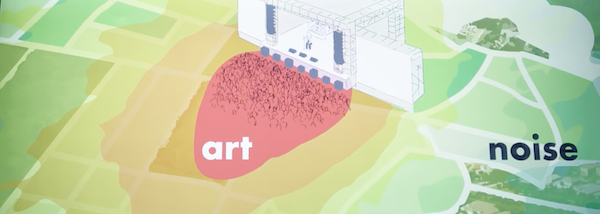
\includegraphics[width=1\textwidth]{change_later.png}
	\caption{Normalized \gls{spl} in colour, red is high \gls{spl} where blue is low \gls{spl}}
		\label{fig:Problem}
\end{figure}

%\autoref{fig:Problem} shows the total sound pressure level \gls{spl} in \gls{db} from \SI{20}{\hertz} to \SI{20}{\kilo\hertz} for the voluntary listeners and the non-voluntary listeners during a concert.
\autoref{fig:Problem} shows a qualitative drawing of a near-ideal sound pressure distribution in the vicinity of a stage during a concert. The high-\gls{spl}areas are highlighted by red color, and is the area where the voluntary listeners condense. This area is define as the \textbf{participants' area} The non-voluntary listeners are located in the area around the participants' area, that we define as \textbf{the neighbourhood}. 

While a \gls{spl} distribution as depicted in \autoref{fig:Problem} is easier to achieve the higher the frequency gets, towards low frequencies the \gls{spl}distribution might look more like depicted in autoref(fig:problem2).



The directivity control of mid- and high frequency has a known solution which has been applied for many years. In general, horns are used, which are designed for a particular radiation pattern. Due to the long wave length in the low/mid- and low frequency range, the horns that are required to direct those wavelengths are not feasible for practical applications due to their size and weight. Therefore other, more space saving solutions have been developed and implemented in the last decade. It is possible to achieve a cardiod emission pattern by arranging subwoofers in a particular manner. Two or three subwoofers are pointed towards the participants' area and one subwoofer is pointed the opposite way. The signal for the subwoofer pointing away from the audience is processed to manipulate the phase.


This project aims towards applying a principle that has been put into commercial use in the D\&B audiotechnik SL-series, where the low/mid frequency directivity is controlled by signal processing four speaker unit. Two units are arranged in the front of the line array module and the other two arranged on each of the sides of the line array module.



\section{preliminary problem statement}
The following questions are made with the intention of gathering the necessary knowledge, to be able to answer a later stated problem statement. The preliminary questions, which will be answered in the analysis, are:

\begin{itemize}
\item In which frequency area do the line source speaker behave omnidirectional?
\item Which known technique is used to do the speaker cardioid?
\item Can a simulation be made which support D\&B audiotechnik claim?
\end{itemize}




%%%
\part{Problem Analysis}\label{pt:analysis} \glsresetall
 \graphicspath{{figures/analysing/}}
	\chapter{Directional characteristics of a loudspeaker}\label{ch:directional}
		\section{Origin}\label{ch:polar_response}
Because this project is about shaping the directional characteristics of loudspeakers arrangements towards a particular direction, it is important to thorougly investigate the directional characteristic of a single loudspeaker. This serves as a baseline for comparison and also is essential, because the investigated loudspeaker will be used to form the speaker array later on.\\
In general, loudspeakers tend to display different directional behaviour depending on the frequency emitted. At low frequencies they can be viewed as omnidirectional sound sources. At higher frequencies the main direction of sound emission is in line with the motion direction of the voice coil. \citep[p. 910 f.]{crocker98}
Depending on the ratio of the emitted wavelength to the diameter of the speaker, a radiation pattern with side lobes can occur. An analytic approximation to the behaviour can be made  when looking at a vibrating piston in an infinite baffel. However, this only takes into account the front side of the speaker. It is difficult to incorporate the effects of an enclosure into this model.\\
There are possibilities to numerically model the sound field around a speaker in a cabinet. However in the context of this project, conducting a measurement seems to be the most favourable approach towards quantifying the sound pressure emitted by loudspeaker mounted in an enclosure. Measurements must be taken at numerous frequencies and positions along a circular trajectory.
For this project, measurements are conducted by placing the test object on a turntable in free field conditions and measuring transfer functions with a microphone. The voltage output of the amplifier and the gain of the microphone can be calibrated so that the only part unknown is transduction performed by the test object. The results of this sort of measurement contain several transfer functions in frequency domain and corresponding impulse responses in time domain. Because they will often be visualized in polar plots, they will henceforth be refered to as the \textit{polar response}.
The knowledge gained through measuring the polar response can then be used in order to designate a feasible frequency range for beamforming in the way that will be described later on. 

\section{Transfer Function Measurement with Sweeps}\label{sec:sweep_theorie}
The characterization of the directional behaviour of the speaker consists of a large number of transfer function measurements. While there are many methods available to obtain transfer functions, it was decided to go with a method that is based on sweeps, due to several benefits. \citep[p. 3 ff.]{mueller01}\\
The sweep signal used for the measurement can be generated by the \gls{ift} of a desired spectrum and a group delay that is designed accordingly. This results in a sinusidal waveform with a continuously altering frequency. In most cases it is desirable to keep a nearly constant amplitude over the whole length of the sweep. The procedure of generating such a sweep signal is illustrated in \autoref{fig:sweep_signal}.

\begin{figure}[htbp]
	\centering
	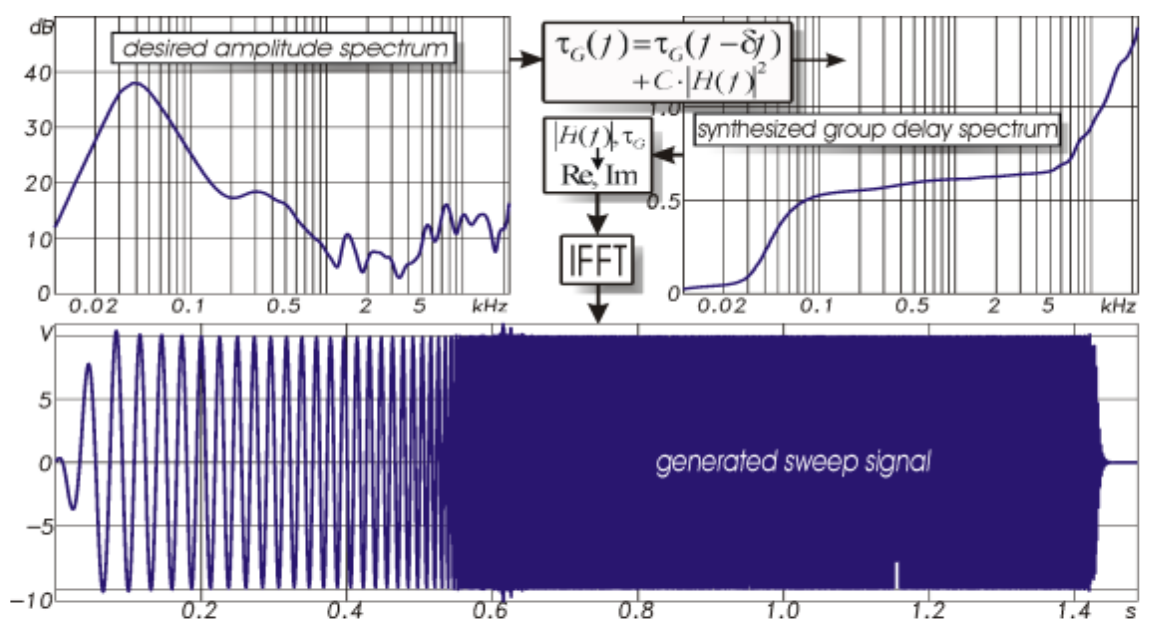
\includegraphics[width=1\textwidth]{mueller01_sweep.png}
	\caption{Sweep synthesis with arbitrary spectral magnitude and nearly constant envelope, taken from \citep{mueller01}}
		\label{fig:sweep_signal}
\end{figure}

The test signal is played back via the loudspeaker that is the test object and the sound is recorded with a microphone in a particular angle towards the main axis of the loudspeaker. An \gls{fft} is performed on the recorded signal. The transfer function of the loudspeaker is then calculated by a multiplication operation with the recorded signal and the inverse of the test signal in frequency domain. It has to be taken into account, that not only the properties of the loudspeaker, but also the distance between the loudspeaker and the microphone and the sound field in the room have an influence on the measurement results. In the context of this project is therefore expedient to conduct the measurements in free field conditions, which means resorting to an anechoic chamber.\\
One particular advantage of sweep measurements over other methods to determine the transfer function is that nonlinearities in the measurement chain or the \gls{dut}, that lead to distortion, can be isolated from the measured transfer function and can be assessed seperately. \citep[p. 20 f.]{mueller01} Simply put, this property is due to the fact, that in the sweep signal, every frequency has a certain group delay, which leads to harmonics being displayed at a negative time when the test signal and the measured signal are convolved in time domain. While it is not the subject of this project to investigate nonlinearities in the behaviour of the speaker in depth, keeping track of the distortion helps with keeping the gains in the measurement chain at a good operating level.

\section{Measurement Setup}\label{sec:meas_setup}
In order to obtain the polar response, transfer functions have to be measured at numerous points. To make measurements more time efficient the loudspeaker is placed on a turntable. The acoustical center (see also \autoref{sec:ac_center}) the loudspeaker is placed on the turning axis. The gain on the microphone amplifier and the input of the soundcard are calibrated, so that a known digital value at the soundcard corresponds to a known sound pressure at the microphone membrane. The gain of the power amplifier that drives the speaker is adjusted, so that a known value at the output of the soundcard corresponds to a known voltage over the terminals of the speaker. With these prerequesits the transfer function can be quantified as sound pressure per voltage at a given distance. The rotation of the turntable, on which the loudspeaker is placed, is controlled by the measurement routine on the computer. After every transfer function measurement, the orientation of the loudspeaker is altered, so that the measurement angles are evenly distributed along the circumference. The measurement data are stored, so that they can be processed into a readable form subsequently.


\begin{figure}[H]
	\centering
\begin{picture}(0,0)%
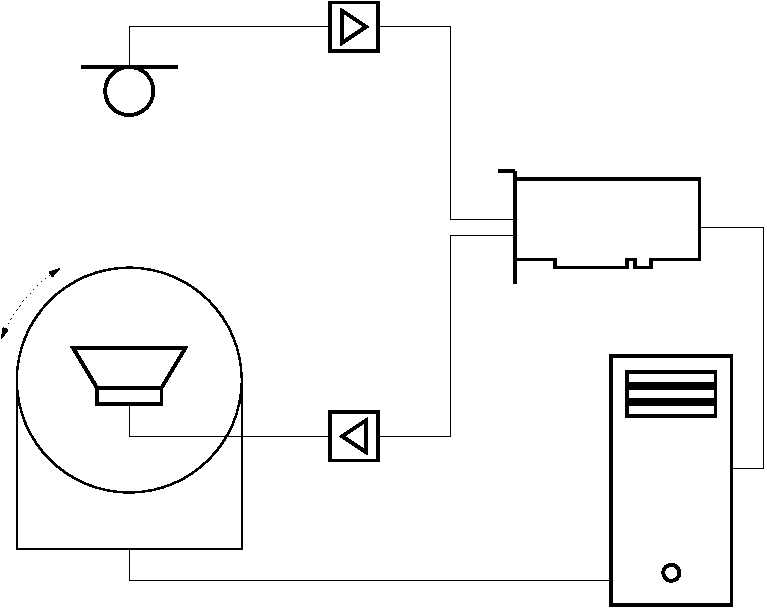
\includegraphics{meas_setup_01.pdf}%
\end{picture}%
\setlength{\unitlength}{2818sp}%
\begingroup\makeatletter\ifx\SetFigFont\undefined%
\gdef\SetFigFont#1#2#3#4#5{%
  \reset@font\fontsize{#1}{#2pt}%
  \fontfamily{#3}\fontseries{#4}\fontshape{#5}%
  \selectfont}%
\fi\endgroup%
\begin{picture}(8570,6816)(3053,-7474)
\put(4900,-1771){Microphone}%
\put(6525,-1501){Amplifier}%
\put(3250,-7081){Turntable}%
\put(6525,-6091){Amplifier}%
\put(9125,-3211){Sound Card}%
\put(10025,-6361){Computer}%
\end{picture}%
\caption{Measurement setup for transfer functions; for convenience the loudspeaker is placed on a turntable, that is controlled by the measurement routine on the computer.}
\label{fig:measurement_setup}
\end{figure}

\section{Determining the Acoustic Center of the \gls{dut}}\label{sec:ac_center}
In order to achieve meaningful results regarding the directional characteristic of the a loudspeaker, it is necessary to know the location of the  acoustic center of the loudspeaker.
In \citep{ansis1.1}, the ``effective acoustical center'' of an electroacoustical transducer is defined as the ``position of the effective or virtual point source from which sound pressure varies inversely as distance''. This concept is further discussed in \citep{jacobsenetal}, where the authors also state, that the position of the acoustic center is frequency dependent. For gathering the data to characterize the directivity it is desirable to position the acoustic center of the \gls{dut} on the rotational axis if the turntable. This can lead to practical difficulties due to the frequency dependency. It is therefore necessary to assess the position of the acoustical center of the \gls{dut} in the desired frequency range via a measurement.\\

Appendix \ref{ax:directional_1} shows the results of a measurement of the polar response that has been conducted without knowing the position of the acoustic center of the \gls{dut} that has been used.
When analyzing the phase data plotted in \autoref{fig:02_23_phase} it seems rather obvious, that the acoustic center of the \gls{dut} has been in front of the rotational axis of the turntable. 
It appears to be possible to estimate the position of the acoustic center by exploiting, that both wavelength and phase at the measurement points on the main axis (\SI{0}{\degree}) and in the opposite direction are known. As described beforehand, the concept of an acoustical center is tied to a  point source, from which waves appear to emerge. If the acoustical center is placed  on the rotational axis, the phase at all microphone positions should have the same value. In the given case it is assumed, that the acoustical center is only off the rotational axis in only the direction of the main axis of the \gls{dut}, and not shifted to the side.
The difference of the phase angles at \SI{0}{\degree} and \SI{180}{\degree} at a given frequency therefore corresponds to a proportion of the wavelength that is double of the distance that the \gls{dut} has to be shifted backwards in order to move the acoustical center onto the rotational axis.
\begin{equation}
S\,=\,\frac{1}{2}\cdot\frac{\phi_0-\phi_{180}}{360^\circ}\cdot\lambda
\end{equation}
\startexplain
    \explain{$S$ is the distance that the \gls{dut} has to be shifted backwards}{\si{m}}
    \explain{$\phi_0$ is the phase angle at the main axis}{\si{\degree}}
    \explain{$\phi_{180}$ is the phase angle at \SI{180}{\degree}}{\si{\degree}}
    \explain{$\lambda$ wavelength}{\si{m}}
\stopexplain    
If \(S\) takes on a negative value, the acoustical center is behind the rotational axis and the \gls{dut} has to be shifted towards the front. There are constraints to the applicability of this concept. The frequency, on which the calculation is based, has to be inside the frequency range at which the speaker can be considered omnidirectional.
The wavelength of the measured frequency can be problematic when it is very long, as the phase difference \(\delta\phi\) between \(phi_0\) and \(phi_{180}\) becomes comparatively small. This leads to a bigger influence to the uncertainty of the phase measurement. On the other hand, comparatively short wavelengths may lead to aliasing effects, when there is a big offset of the center from the rotational axis. However this does not to be so relevant in practical application, because towards higher frequencies, loudspeakers tend not to behave like omnidirectional sources.\\
In \autoref{tab:shift_meas1}, data from the measurement described in Appendix \ref{ax:directional_1} has been used to calculate the offset of the acoustical center from the rotational axis of the turntable at three different frequencies. The wavelengths \(\lambda\) were based on the assumption, that the speed of sound was \(c\,=\,\)\SI{343}{\meter\per\second}, corresponding to a temperature \(T\,\approx\,\)\SI{20}{\celsius}. The results for all three frequencies are rather similar.
\begin{table}[H]
\centering
\caption{Calculation of the offset of the acoustic center based on Appendix \ref{ax:directional_1}}
\label{tab:shift_meas1}
\begin{tabular}{|lr|r|r|r|}
\hline
Frequency              & {[}Hz{]}  & 60    & 100    & 150    \\ \hline
\(\phi_0\)             & {[}Deg{]} & 58.8  & 341.1  & 266.1  \\ \hline
\(\phi_{180}\)         & {[}Deg{]} & 17.2  & 269.7  & 159.9  \\ \hline
\(\Delta\phi\)         & {[}Deg{]} & 41.6  & 71.4   & 106.2  \\ \hline
\(\lambda\)            & {[}m{]}   & 5.72  & 3.43   & 2.29   \\ \hline
\(S\)                  & {[}m{]}   & 0.330 & 0.340  & 0.337  \\ \hline
\end{tabular}
\end{table}
Comparing \(S\) with the positioning of the speaker relative to the rotational axis during the measurement would allow for specifying the estimated position of the acoustic center. However, there was some significant undesired mechanical flexibility in the way the speaker was mounted, which lead to imprecisions (see \autoref{fig:setup_02_23}). Therefore, another mechanical solution was implemented and the measurement was repeated. This is  logged in Appendix \ref{ax:directional_2}.
During this second measurement campaign the speaker was placed further to the back to get the acoustical center closer to the rotational axis. However, there is still some offset, as can be seen in \autoref{tab:shift_meas2}.
Adding \(S\) to the distance between  the front plane of the cabinet and the rotational axis, a rough estimate of the position of the acoustic center in relation to the front plane of the cabinet \(C\,\approx\,\)\SI{0.17}{\meter} can be made. As there were still some mechanical weaknesses involved and the temperature during the measurement was unknown, this estimate has to be confirmed in a final measurement campaign, where the speaker is set back according to the findings of \autoref{tab:shift_meas2}.\\
One aspect that has to be mentioned in this context is the dependency of the acoustic center on frequency. According to the findigs of \citep{vanderkooy10}, who has done a boundary-element calculation of the acoustic center, the frequency dependent position alteration can be deemed  neglegible for the sake of this project.
\begin{table}[H]
\centering
\caption{Calculation of the offset of the acoustic center based on Appendix \ref{ax:directional_2}}
\label{tab:shift_meas2}
\begin{tabular}{|lr|r|r|r|}
\hline
Frequency              & {[}Hz{]}  & 60    & 100    & 150   \\ \hline
\(\phi_0\)             & {[}Deg{]} & 108.9 & - 60.8 & 138.0 \\ \hline
\(\phi_{180}\)         & {[}Deg{]} & 103.3 & - 70.8 & 126.5 \\ \hline
\(\Delta\phi\)         & {[}Deg{]} & 5.6   & 10     & 11.5  \\ \hline
\(\lambda\)            & {[}m{]}   & 5.72  & 3.43   & 2.29  \\ \hline
\(S\)                  & {[}m{]}   & 0.044 & 0.048  & 0.037 \\ \hline
\end{tabular}
\end{table}
%A way to determine the acoustical center by measurement can be proposed as follows. The loudspeaker is placed on the turntable, oriented with its main axis directly towards the measurement microphone (\SI{0}{\degree}). Details about this procedure can be found in \autoref{ax:directional_1}.


\section{Determining the beamwidth of the \gls{dut}}\label{sec:ac_center}
In order to find the beamwidth of the \gls{dut}, a pre polar response measurement have to be done to localize the acoustic center of the \gls{dut} by analyse the polar phase of the \gls{dut}. With the knowledge of the polar phase to a given frequency, it is possible to calculate the distance in x and y direction, the \gls{dut} have to be moved. The pre polar response is explained in \autoref{ax:directional_1}, and in \autoref{} the moment was calculated to ... in x direction and ... in y direction. 
After the speaker is moved to the calculated position, the polar response is measured again and analysed in \autoref{ax:directional_2}. Because of flexibility of the first stand in \autoref{ax:directional_1}, the position of the speaker is of with \SI{4.5}{\centi\meter} to the front. The measurement  is executed according to \autoref{appendix:beamwidth} and the beamwidth of the \gls{dut} is as following \autoref{fig:beamwidth_offset_4.5_cm} 

\begin{figure}[htbp]
	\centering
	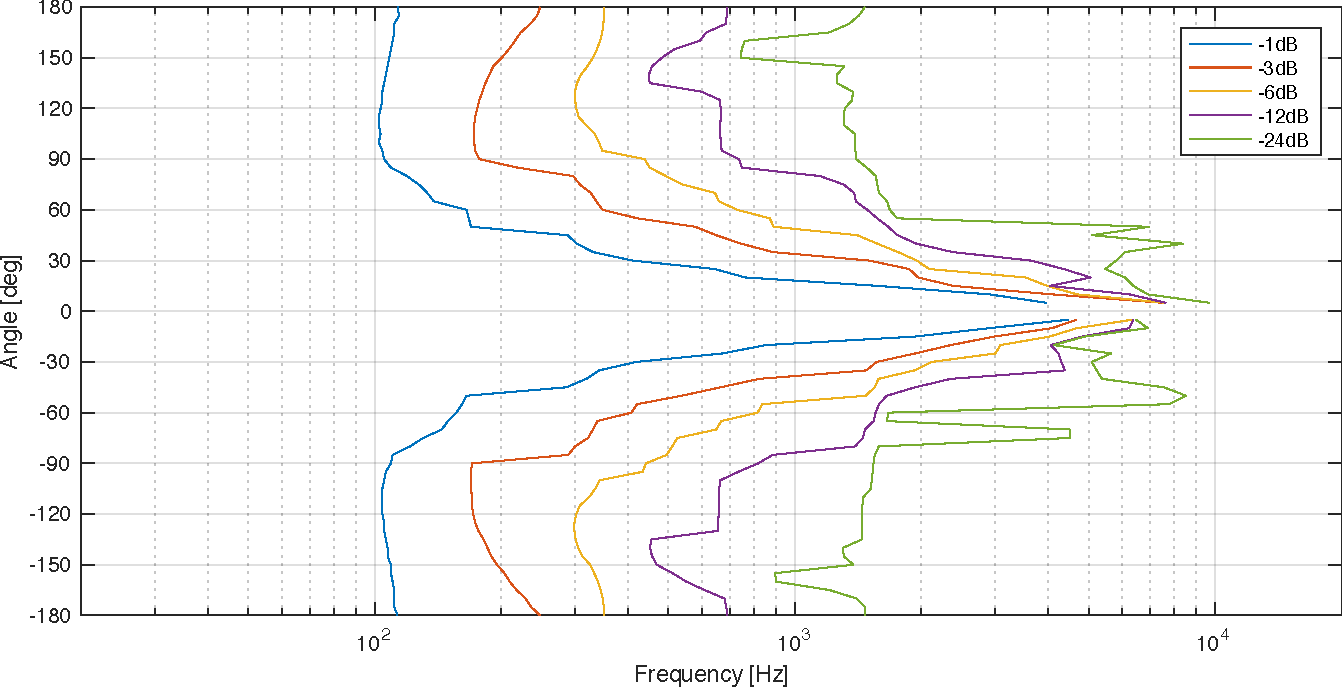
\includegraphics[width=1\textwidth]{beamwidth_off_4_5_cm.pdf}
	\caption{The figure shows the beamwidth to a specified \si{\decibel} change between the front measurement and a measurement from a given angle of the \gls{dut}. It find the first frequency where the \gls{spl} difference between front measurement and the measurement from the given angle is $n$\si{\decibel}, where $n$ is given in the figure. The \gls{dut} which correspond to this figure is a \citep{seas33}}
		\label{fig:beamwidth_offset_4.5_cm}
\end{figure}

		\section{Conclusion of directional characteristic}
Several measurements (see Appendices \ref{ax:directional_1} \& \ref{ax:directional_2}) were conducted on the loudspeaker configuration, consisting of a \citep{seas33} inside a (400x400x400)\si{\milli\meter} cabinet. The loudspeaker proved to be suitable for sound playback in the frequency range of \SIrange{60}{300}{\hertz} that is the focus of this project.\\
The directivity within this frequency range is shown to be very unfocused. With a threshold of \SI{-1}{\decibel} the loudspeaker can even be regarded as an omnidirectional source up to approx \SI{100}{\hertz}. With a higher threshold of \SI{-3}{\decibel} this upper frequency limit is approx. \SI{200}{\hertz}. By implication this means, that the behaviour of the speaker cannot be described as omnidirectional above the formerly mentioned frequencies.
For the grand scheme of things this means, that it is likely possible to prove the concept of three-speaker-beamforming in the lower part of the selected frequency range. However in the higher part of the frequency range, adaptions to the non-omnidirectional characteristics of the speaker have to be implemented in order to achieve satisfactory results.
	\chapter{Analytical descriptions}\label{ch:analytical}
		\section{Single source}\label{ch:single_speaker_source}
To gain understanding about the interaction of several sources emitting sound simultaneously it is essential to first investigate the behaviour of a singular sound source. In the context of this project loudspeakers are investigated. The goal of this section is to find a way to represent the sound emission of loudspeakers within the frequencies boundaries of this project (\SIrange{60}{300}{\hertz}).
The representation must be suffiencently accurate yet relatively simple to calculate in order to be useful in the optimization process that is a later part of this project (see \autoref{ch:optimization}).

%This section aims to introduce and analyse the fundamental for a single source, by analyse the behaviour of a baffled circular plane piston source. The pressure around the piston source will be analysed analytically, to determine the radiation of a single speaker from \SI{60}{\hertz} and upwards and compare it with the measurement from \autoref{ch:polar_response}. The \SI{60}{\hertz} lower limit enable the simulation to be validated by measurement in the AAU anechoic chamber and is a used lower limit for the low/mid driver in some line source array \citep{V-DOSC}.  The analyse shall end out with a approximated simulation model of the \gls{dut}.
\subsection{Pressure emission from an omidirectional source}
As explained in \autoref{ch:polar_response} loudspeakers are commonly treated as omnidirectional sources at low frequencies. Taking advantage of this approximation, the sound pressure emission in free field conditions can be described conveniently. \citep[p. 171]{Kinsler2000} state the following equation \autoref{eq:omni_source} for a pulsating sphere. It has to be noted, that the position of the sphere in the given case is the acoustic center of the loudspeaker (see \autoref{sec:ac_center}).
\begin{equation}\label{eq:omni_source}
p(r,t)\,=\,\rho_0 c V_0 \left(\frac{a}{r}\right)\cos \theta_a \textbf{\textit{e}}^{j\left(\omega t - k(r-a)+\theta_a\right)}
\end{equation}
\startexplain
\explain{$p$ is the sound pressure.}{\si{\pascal}}
\explain{$r$ is the distance, for which the pressure is being calculated, \(r>a\).}{\si{\meter}}
\explain{$t$ is the time, for which the pressure is being calculated.}{\si{\meter}}
\explain{$\rho_0$ is the specific density of air.}{\si{\kilo\gram\per\cubic\meter}}
\explain{$c$ is the speed of sound.}{\si{\meter\per\second}}
\explain{$V_0$ ist the peak velocity at the surface of the spherical source.}{\si{\meter\per\second}}
\explain{$a$ is the radius of the spherical source.}{\si{\meter}}
\explain{$\theta_a$ is equal to $\tan(ka)$.}{\si{1}}
\explain{$\omega$ is the angular frequency.}{\si{\second^{-1}}}
\explain{$k$ is the wavenumber.}{\si{\meter^{-1}}}
\stopexplain

\subsection{Pressure emission from a baffled piston}
Another  approach to analytically approximate the behaviour of a cone loudspeaker is given by \citep[p. 179 ff.]{Kinsler2000}, where the behaviour of the sound radiated from a plane circular piston surrounded by an infinte rigid baffle is described.


%To characterize the directional properties of an analytical model of the \gls{dut}, the source will be modulated in two dimension as one baffled circular plane piston source. The analysis of a piston source in two dimension built on a thin piston source in three dimension where the x axis is fixed in the plot. This is possible because of vertical beam patten symmetry of \autoref{fig:continues_line_source} \citep{Kinsler2000}. The piston lays flat down so i look like a line source and have radius $a$. The baffled circular plane piston source can be considered as many continuous line sources, which detonate dx and is pointing towards the reader on \autoref{fig:continues_line_source}. The calculated pressure point will be in far field where $r>>a$ holds and the surface integral can be rewritten to a Bessel function \citep{Kinsler2000}. The pressure formula is therefore:

\begin{equation}
p(r,\theta ,t)=\frac{j}{2} \rho_{0}c  V_{0}\frac{a}{r}ka \left ( \frac{2J_1(ka\, sin(\theta ))}{ka\, sin(\theta )} \right )e^{j(\omega t-kr)}
\end{equation}
Where the complete surface vibration is described with

\begin{equation}
v = V_{0} \cdot exp(j \omega t)
\end{equation}

\startexplain
    	\explain{$v$ is the complex speed of the line source }{\si{1}}
        \explain{$V_{0}$ is the Amplitude}{\si{1}}
        \explain{$j$ is the imaginary unit }{\si{1}}
        \explain{$\omega$ is the angular velocity }{\si{1}}
        \explain{$t$ is the time }{\si{1}}
\stopexplain
    
Each small sources is treated as an baffled simple source with a width of $dx$ and the source strange can be modulated as following      

\begin{equation}
dQ = V_{0} 2 a\, sin(\phi) \, dx
\end{equation}

    \startexplain
    		\explain{$dQ$ is the simple source strange }{\si{1}}
        \explain{$V_{0}$ is the Amplitude}{\si{1}}
        \explain{$a$ is the radius for cylinder }{\si{1}}
        \explain{$\phi$ is the angle between the radius $a$ and the x axis}{\si{1}}
        \explain{$dx$ is the length for the simple source }{\si{1}}
    \stopexplain    
 
The following \autoref{fig:continues_line_source} shows an example of the continues line source where one of the small source is showed with width $dx$ and length $2a \, sin(\phi)$. 

\begin{figure}[H]
	\centering
\begin{picture}(0,0)%
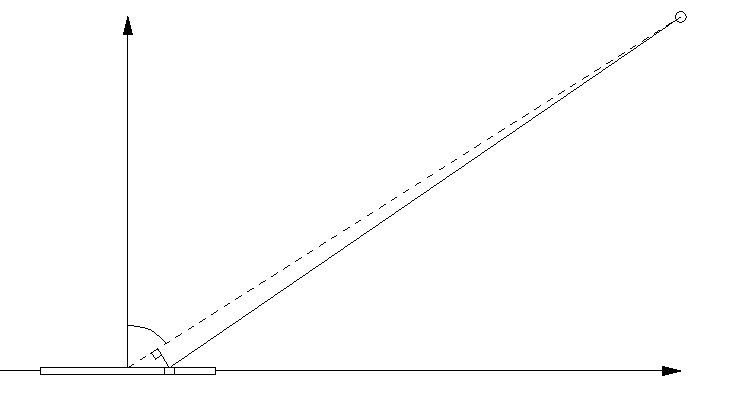
\includegraphics{line_source.pdf}%
\end{picture}%
\setlength{\unitlength}{746sp}%
%
\begingroup\makeatletter\ifx\SetFigFont\undefined%
\gdef\SetFigFont#1#2#3#4#5{%
  \reset@font\fontsize{#1}{#2pt}%
  \fontfamily{#3}\fontseries{#4}\fontshape{#5}%
  \selectfont}%
\fi\endgroup%
\begin{picture}(31223,16833)(-5411,-436)
\put(12106,7139){r'}%
\put(24121,15599){P(r,$\theta$,t)}%
\put(946,2684){$\theta$}%
\put(23851,659){x}%
\put(-89,16094){z}%
\put(11341,8354){r}%
\put(3466,-571){$a$}%
\put(1441,-376){$dx$}%
\put(-134,-421){0}%
\put(-4049,-571){$-a$}%
\put(226,1649){$\Delta$r}%
\end{picture}%
	\caption{The model of a continues line source where y axis is pointing towords the reader. (ref the book)}
		\label{fig:continues_line_source}
\end{figure}




\subsection{Simulation of the \gls{dut} as a piston source and compare to measurement in \autoref{ch:polar_response}}
In this section, the \gls{dut} will be simulated as a baffled circular plane piston source as described in \autoref{ch:single_speaker_source} and compared to the actually measurement of the \gls{dut} \autoref{ax:directional_2}. An piston simulated model of \citep{seas33} in MATLAB shows in \autoref{fig:piston_model_of_seas33}

\begin{figure}[H]
	\centering
	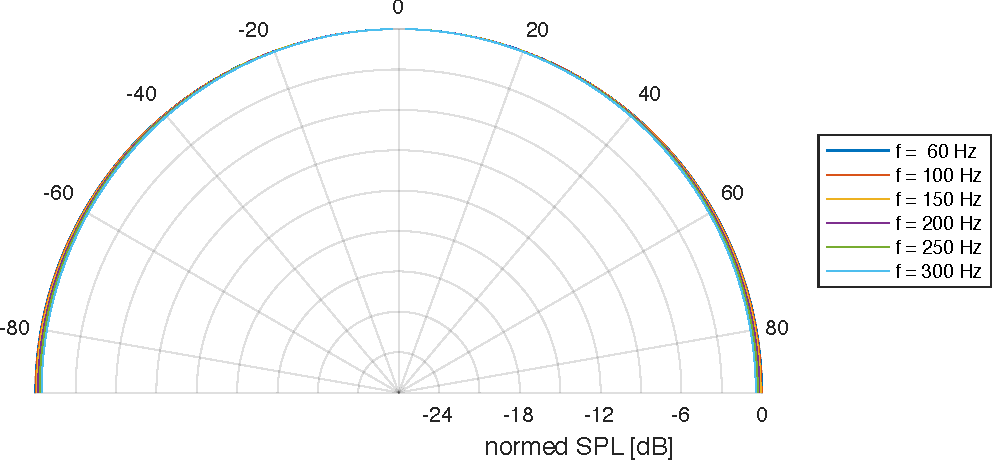
\includegraphics[width=0.8\textwidth]{piston_model.pdf}
	\caption{The figure shows  The \gls{dut} which correspond to this figure is a \citep{seas33}}
		\label{fig:piston_model_of_seas33}
\end{figure}

The actually measurement of the \citep{seas33}  \autoref{ax:directional_2}.

\begin{figure}[H]
	\centering
	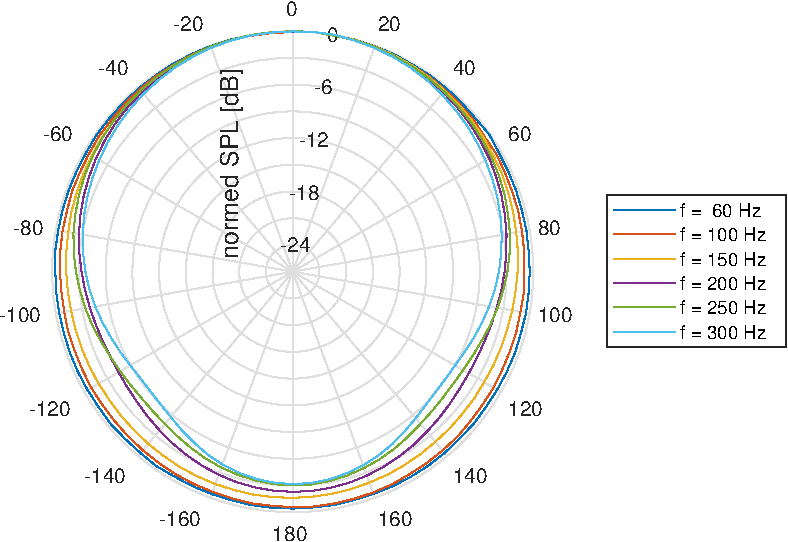
\includegraphics[width=0.8\textwidth]{meas1_seas.pdf}
	\caption{The figure shows  The \gls{dut} which correspond to this figure is a \citep{seas33}}
		\label{fig:speaker_model}
\end{figure}

\subsection{Conclusion}
		\section{zero order gradient speaker}
		\section{First order gradient speaker}
		\section{The dimension limit} 

	



%%
\part{Design and Optimization}\label{pt:design} 
\graphicspath{{figures/design/}}
	\chapter{Hardware Configuration}
		%\section{Digital Signal Processor Choice}

The chosen component is the \gls{dsp} for numerous reasons that are going to be presented in the following subsections.

\subsection{Advantage of the \gls{dsp} over the FPGA}

Some of the  reasons of choosing a \gls{dsp} over an FPGA in this project are:
 
\begin{itemize}

\item  The simplicity of designing with a \gls{dsp} due to the availability of all the simple functionalities in a micro-controller \citep{eetimes}. 

\item A \gls{dsp} is designed to perform signal processing tasks unlike the FPGA which purpose of creation was not related to signal processing but to program circuits \citep{eetimes}. 

\item A \gls{dsp} is more suitable in terms of cost/performance, when the application has less than 3000 \gls{mmac} per second, which means that it is better for low demanding applications \citep{eetimes}. 

\item FPGA's lack integrated DAC and ADC \citep{eetimes}. 

\item The \gls{dsp}'s are more power efficient than the FPGA's which can be important if the effect is to be used on the move on battery power \citep{rtcmag}. 

\item A \gls{dsp} can be optimal if there are many operations that are repeated \citep{eetimes} \citep{hunteng}. 

\end{itemize}

\subsection{Advantage of the \gls{dsp} over the Raspberry Pi}

Some of the  reasons of choosing a \gls{dsp} over a Raspberry Pi in this project are:
 
\begin{itemize}

\item \gls{dsp}'s are much faster for integer and floating mathematical calculations. \gls{dsp}'s are designed to compute large and complex operations that are repetitive which makes it more suitable for this project \citep{diffbet} \citep{esp_simone}.   

\item A micro-controller, such as a Raspberry Pi, has many different features that are not going to be used in the project \citep{diffbet} \citep{esp_simone}. 

\item In general, a \gls{dsp} is faster than a micro-controller, for signal processing, because it involves specialized units like multipliers \citep{diffbet2}. 

\item A micro-controller is usually used for control applications and not signal processing even if it can work \citep{tex_dsp}.

\end{itemize}












	\chapter{Determining SP-Parameters}\label{ch:optimization}
		\section{Problem Description}
In order to realize a directional low-mid emission with three near-omnidirectional speakers, signal parameters have to be chosen in a specific manner. The directional characteristics of the speaker array depend on the amplitude and phase of the signal that is transduced via the individual speakers. The resulting directional characteristics of a given set of signal-parameters can be described by the use of an analytical model, that has been supplemented with knowledge from measuring the polar response of the speakers (see \autoref{sec:correction}).\\
Assuming, that the model describing the directional characteristics of the array is sufficiently accurate, it is possible to form an optimization problem. Any set of \gls{sp} parameters can be evaluated by plugging it into the augmented analytical model, which will be used to form an objective function. Solutions, that resemble the desired directional characteristic are considered optimal.\\
The augmented analytical model incorporates correction data from a table. Because setting up the model is a step that is done in an early stage of this project, it is not unlikely that modifications have to be made.  This makes it favourable to approach the given problem with combinatorial optimization, which allows for changes in the objective function to be implemented easily. Specifically, it has been chosen to handle the problem with a \gls{ga}, where the augmented analytical model used to evaluate the \textit{fitness}.
This decision is based on the \gls{ga} being a more flexible approach compared to finding a specific way of solving the optimization problem as a continuous problem. When using a \gls{ga}, changes in the objective function can be accounted for with relatively little effort. This is especially handy in a development process like it is the case in this project. The basic framework of the optimization stays the same, while changes to the speaker configuration, definition of the cost, and mathematical representation of the sound radiated from the speaker can be made. In this project this has been the case with the introduction of the augmented speaker model in \autoref{sec:correction}. The use of a correction table would introduce difficulties when trying to approach the optimization as a continuous optimization problem.

\section{\gls{ga}: Fundamentals}\label{sec:ga_fundamental}
In \citep[p. 7]{goldberg89}, the author designates four main properties in order to elucidate genetic algorithms. 
\begin{enumerate}
\item \gls{ga}s rely on coded parameter sets, not the actual parameters themselves.
\item \gls{ga}s work with a \textit{population} of solutions, not a single one.
\item \gls{ga}s only require an objective function to evaluate the fitness of the solutions, not its derivative or other auxilary information.
\item \gls{ga}s utilize probabilistic transition rules for generating new solutions, as opposed to determinstic transitions.
\end{enumerate}
These points outline the fundamental idea of a \gls{ga}s. A pool of solutions to a given problem evolves over a number of generations via probabilistic transition rules (\textit{crossover}, \textit{mutation}).
These transition rules rely on evaluating the fitness of the solutions with the objective function in order to adjust the probabilities so that desirable properties are likely to subsist.
\citep{genetic_survey}

\section{Implementation: Approach and Structure}\label{sec:genetic_implememtation}
\definecolor{green3}{rgb}{0,0.56,0}
In order to set up a \gls{ga}, the \textit{phenotypes}, which are real world solutions to a real world problem, have to be coded into \textit{genotypes}, which represent those \textit{phenotypes} in a mathematical form. This corresponds to the coded parameter sets that are mentioned in point 1. in \autoref{sec:ga_fundamental}.
A way to describe the acoustical beamforming problem, that this project is investigating, is illustrated in \autoref{fig:gene_setup}. The parameters, that make up the genotypes, are denoted in \textcolor{green3}{green} letters. The hardware setup consists of three loudspeakers (A,B,C). Each of the speakers is fed with a signal, that is a modified version of a common source signal. The signals differ in gain (\textcolor{green3}{\texttt{Va}}, \textcolor{green3}{\texttt{Vb}}, \textcolor{green3}{\texttt{Vc}}) and phase (\textcolor{green3}{\texttt{Phia}}, \textcolor{green3}{\texttt{Phib}}, \textcolor{green3}{\texttt{Phic}}). The positioning of the \textcolor{red}{acoustic centers} of the loudspeakers relative to each other is set up as a isosceles triangle. The triangle is described using the length of its base side (\textcolor{green3}{\texttt{Lx}}) and the corresponding height (\textcolor{green3}{\texttt{Ly}}). Negative values of \textcolor{green3}{\texttt{Ly}} mean, that the tip of the triangle is pointing in the opposite direction compared to the setup in \autoref{fig:gene_setup}. When referring to genetic algorithms, the formerly mentioned parameters are commonly refered to as \textit{genes}. The particular value, that each of the genes has in a genotype is referred to as an \textit{allele}. The set of genes are refered to as \textit{chromosomes}. In this particular case, each individual genotype has just one chromosome and the alleles are represented in \SI{64}{\bit} floating-point values.\\
Because the genetic algorithm works with a pool of solutions at any given time, it is necessary to initialize a population of genotypes. This corresponds to point 2. in \autoref{sec:ga_fundamental}. The way, that the population is initialized in the algorithm used for this project, is shown in Appendix \ref{axs:pop_init}. The initial alleles are determined with some random values that are combined with some educated guessing (see also \autoref{sec:ga_prior}).\\
\begin{figure}[H]
	\begin{sideways}
	\begin{minipage}{\textheight}
%		\centering
\begin{picture}(0,0)%
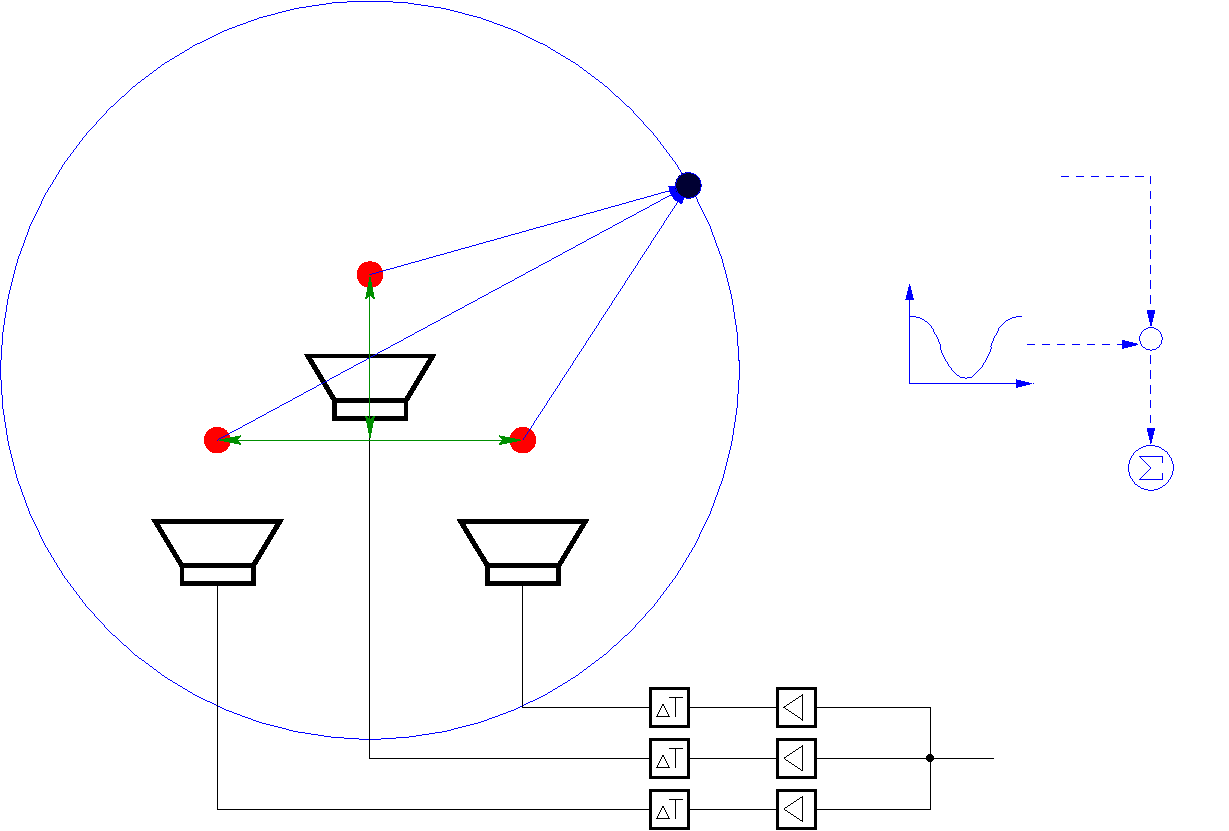
\includegraphics{genetic_setup_01.pdf}%
\end{picture}%
\setlength{\unitlength}{3937sp}%
\begingroup\makeatletter\ifx\SetFigFont\undefined%
\gdef\SetFigFont#1#2#3#4#5{%
  \reset@font\fontsize{#1}{#2pt}%
  \fontfamily{#3}\fontseries{#4}\fontshape{#5}%
  \selectfont}%
\fi\endgroup%
\begin{picture}(9844,6664)(-681,-4729)
\put(8509,-860){\makebox(0,0)[lb]{\smash{{\SetFigFont{20}{20.0}{\rmdefault}{\mddefault}{\updefault}{\color[rgb]{0,0,1}$\cdot$}%
}}}}
\put(2701,-1411){{\color[rgb]{0,0,0}Speaker A}%
}
\put(1441,-2761){{\color[rgb]{0,0,0}Speaker B}%
}
\put(3871,-2761){{\color[rgb]{0,0,0}Speaker C}%
}
\put(5941,-3661){{\color[rgb]{0,.56,0}\texttt{Va}}%
}
\put(5941,-4066){{\color[rgb]{0,.56,0}\texttt{Vb}}%
}
\put(5941,-4471){{\color[rgb]{0,.56,0}\texttt{Vb}}%
}
\put(4906,-4471){{\color[rgb]{0,.56,0}\texttt{Phic}}%
}
\put(4906,-4066){{\color[rgb]{0,.56,0}\texttt{Phib}}%
}
\put(4906,-3661){{\color[rgb]{0,.56,0}\texttt{Phia}}%
}
\put(2341,-601){{\color[rgb]{0,.56,0}\texttt{Ly}}%
}
\put(1081,-331){{\color[rgb]{1,0,0}Ac. Center A}%
}
\put(-179,-1681){{\color[rgb]{1,0,0}Ac. Center B}%
}
\put(3691,-1681){{\color[rgb]{1,0,0}Ac. Center C}%
}
\put(5131,659){{\color[rgb]{0,0,1}Pressure along the circumference}%
}
\put(5131,404){{\color[rgb]{0,0,1}of the array, calculated according}%
}
\put(5131,149){{\color[rgb]{0,0,1}to the augmented pressure equation \ref{eq:aug_omni}}%
}
\put(1801,-1771){{\color[rgb]{0,.56,0}\texttt{Lx}}%
}
\put(6436,-1366){{\color[rgb]{0,0,1}weighting curve}%
}
\put(8056,-2176){{\color[rgb]{0,0,1}fitness value}%
}
\end{picture}%
	\end{minipage}
	\end{sideways}
%\center
\caption{Phenotype and Genotype relations, visualization of genes and fitness evaluation. Alleles are denoted in \textcolor{green3}{green} and the fitness evaluation method is denoted in \textcolor{blue}{blue}.}
\label{fig:gene_setup}
\end{figure}
According to point  3. in \autoref{sec:ga_fundamental}, there needs to be a function that evaluates the fitness of every genotype based on some criteria. The way that this is achieved is also visualized in \autoref{fig:gene_setup}. The corresponding code is shown in Appendix \ref{axs:fitness}. The coordinates of a \textcolor{blue}{circle} around the centroid of the triangle between the \textcolor{red}{acoustic centers} are calculated. The position of the centroid will from now on be related to as the \textit{array center}. The radius of the \textcolor{blue}{circle} is significantly larger than the size of the speaker array. In this project, the chosen radius is \SI{10}{\meter} for both the analytical model and the simulation. From coordinates on the circumference, a set of coordinates, that describes the distance to each \textcolor{red}{acoustic center}, is deduced for each of the speakers. Using these coordinates, the gain and phase parameters from the alleles as well as the frequency, for which the optimization is excecuted, the pressure from each speaker is calculated using \autoref{eq:aug_omni}. The pressures are added in order to get the resulting pressure along the circumference. At this point it is crucial to take intro account the phase and therefore it is not the absolute pressure but the complex pressure that is summed.\\
The ultimate goal of running this \gls{ga} is getting a phenotype solution, that leads to particular desired directional characteristics of the speaker array. The desired characteristics are specified, by weighting the normed absolute pressure along the circumference according to some preference. This means, pressure in the direction in the direction, in which sound emission is desired, is assigned a low cost, whereas pressure in a direction, in which sound emission is undesired, is assigned a high cost. When the normed and weighted pressure is summed, a fitness value is calculated. The formerly described way of applying weight leads to lower values corresponding to fitter solutions.\\
The final point 4. from \autoref{sec:ga_fundamental} mentions probabilistic transition rules. The implementation of these is shown in Appendices \ref{axs:parents}, \ref{axs:offspring} and \ref{axs:mutation}. The genotypes, that are used to generate new genotypes for the subsequent generation are selected via tournament
selection \citep{tournament}. This ensures plenty of randomness while there is still some pressure caused by the fitness of the individual solution.
Offspring is then generated by combining the alleles of the parent genotype at a randomly determined ratio. This leads to two offspring genotypes with complementary ratios.
Furthermore there is a mutation function, that, with a comparatively low probability, changes one of the allele of any genotype to a randomly determined value.\\
A number of generations are computed after the initialization. The most fit genotype of the last generation that is computed should represent a near optimal solution to the beamforming problem. It has to be noted, that this routine has to be repeated for every frequency, for which a set of parameters is to be obtained.



\section{Inclusion of Prior Knowledge}\label{sec:ga_prior}
To simplify the optimization task, it is expedient to exploit knowledge and requirements given from the context of the project. This prior knowledge contains constraints that are given by practical issues. This leads to constraints, like the maximum distance between the acoustic centers, that is determined by the size of the anechoic chamber, in which the speaker array should be set up for measurements, or the minimum distance between the acoustic centers, which is determined by the physical size of the loudspeakers. It is possible to use the optimization to obtain parameters that lead to a main emission direction of the speaker array in any direction. However, for practical reasons the preferred solutions have either a single speaker on the line between the array center and main emission direction, or the connecting line between two acoustic centers perpendicularly to the formerly mentioned main emission direction. This leads to a symmetrical array configuration, which means, that optimal signal processing parameters are assumed to be equal for two of the three speakers. Implementing the \gls{ga} with this in mind, the optimization can be simplified.
Another form of prior knowledge is used when initializing the population. With trial-and-error style heuristics, some knowledge about the nature of fit solutions can be gained and implemented in the initialization function as an expectational value when setting up parameters as Gaussian random variables.\\
Prior knowledge is also incorporated in the way that the optimization is excecuted over the whole frequency range of \SIrange{60}{300}{\hertz}. Heuristic trials have shown, that the placement of the loudspeakers is much more critical for the optimization result at higher frequencies then it is at lower frequencies. When it is intended to actually set up a speaker array that is driven the signal processing parameters that are the result of the optimization process, and measure and experience the performance, then it is not feasible to have different speaker positions for different frequencies. For this reason it was initially planned to start the optimization process at the highest frequency. The speaker position would then be fixed. In the following optimization runs, only gain and phase are optimized. Using the population of the last generation from the previous frequency optimization, allows to have a smaller number of generations when optimizing for the adjacent frequency as some of the genotypes are already close to optimal. 
However, it has to be taken into account, that a comparison between the analytical model of the array and some \gls{fdtd}-simulation results is part of this project (see \autoref{sec:meas_vs_theory}). This leads to a discretization of the feasible values for the alleles \textcolor{green3}{\texttt{Lx}} and \textcolor{green3}{\texttt{Ly}}. This is not ideal for the implementation in this particular genetic algorithm. Additionally, the main axis response, as it is described in the next Section \ref{sec:main_axis}, leads to practical issues, where it is undesirable to apply significantly more voltage to speakers in at particular frequencies then at others. This has lead to the decision to fix the position according to a criterion related to the main axis response (see \autoref{ssec:cost_map}).


\section{Main axis response}\label{sec:main_axis}
\subsection{Analytical Considerations}\label{ssec:main_axis_formulas}
To assess the practicability of the speaker array, it can be investigated, how it behaves on the main axis, where the voluntary audience is assumed to be. In order to do this, the frequency dependent sound pressure level on the main axis $L_{p,beam}(f)$ is compared a reference pressure level $L_{p,ref}(f)$, that is emitted by three loudspeakers of the same kind as those in the array, placed closely together as illustrated in \autoref{fig:ref_omni_array}. These analytical considerations are undertaken using augmented omnidirectional sources (\autoref{eq:aug_omni}). The velocity for this reference sources is the same, as the one for two frontal sources of the array. In the reference case, all three sources are in phase.
We can introduce the frequency dependent beamforming cost $\Delta L_{p}(f)$ as the difference between the reference level $L_{p,ref}(f)$ and the beamformed level $L_{p,beam}(f)$ (see \autoref{eq:beam_cost}).  The beamformed level is a pressure level calculated similarly to the cost function in the optimization. The speakers are arranged triangularly and the velocity for speakers B and C is the same as in the formerly mentioned reference case, whereas the velocity and phase of speaker A are set according some optimization result. This case is illustrated in \autoref{fig:ref_caridioid_array}. For all calculations, a distance of $r\,=\,\SI{10}{\meter}$ will be used.
\begin{equation}\label{eq:beam_cost}
\Delta L_{p}(f)\,=\,L_{p,ref}(f)-L_{p,beam}(f)
\end{equation}

\begin{figure}[h]
	\centering
\begin{picture}(0,0)%
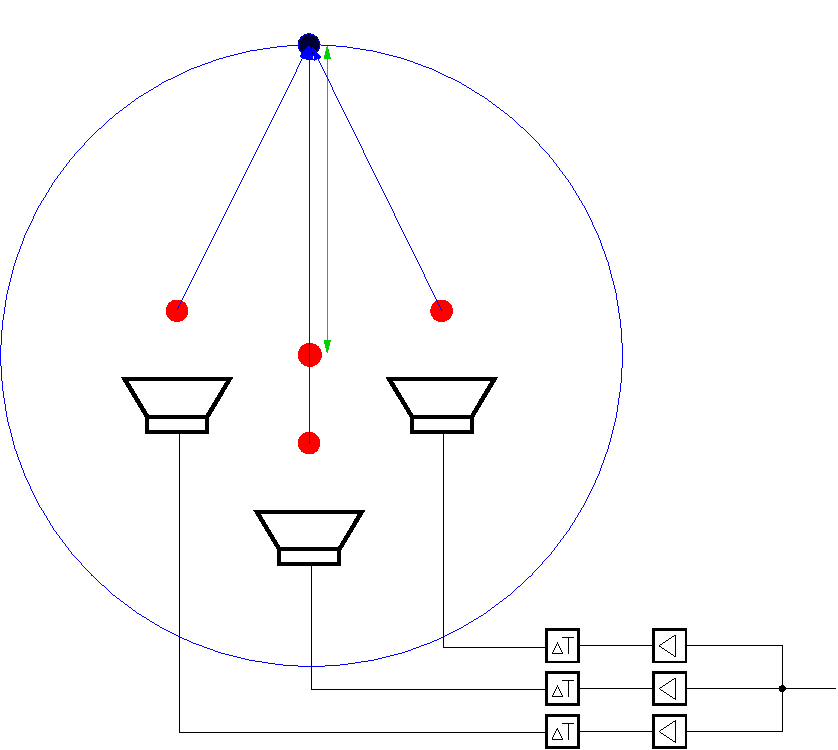
\includegraphics[scale=0.5]{ref_caridioid_array.pdf}%
\end{picture}%
\setlength{\unitlength}{1658sp}%
%
\begingroup\makeatletter\ifx\SetFigFont\undefined%
\gdef\SetFigFont#1#2#3#4#5{%
  \reset@font\fontsize{#1}{#2pt}%
  \fontfamily{#3}\fontseries{#4}\fontshape{#5}%
  \selectfont}%
\fi\endgroup%
\begin{picture}(7975,7142)(-672,-4729)
\put(5941,-3661){\color[rgb]{0,.56,0}\scriptsize{\texttt{Va}}}%
\put(5941,-4066){\color[rgb]{0,.56,0}\scriptsize{\texttt{Vb}}}%
\put(5941,-4471){\color[rgb]{0,.56,0}\scriptsize{\texttt{Vb}}}%
\put(4906,-4471){\color[rgb]{0,.56,0}\scriptsize{\texttt{Phib}}}%
\put(4906,-4066){\color[rgb]{0,.56,0}\scriptsize{\texttt{Phib}}}%
\put(4906,-3661){\color[rgb]{0,.56,0}\scriptsize{\texttt{Phia}}}%
\put(2271,2230){\color[rgb]{0,0,0}$L_{p,beam}$}%
\put(2535,219){\color[rgb]{0,.82,0}\SI{10}{\meter}}%
\put(2566,-1051){\color[rgb]{1,0,0}Array center}%
\put(2386,-3511){\color[rgb]{0,0,0}Speaker A}%
\put(1056,-2196){\color[rgb]{1,0,0}Ac. Center A}%
\put(-1150,-1051){\color[rgb]{1,0,0}Ac. Center B}%
\put(-1000,-2251){\color[rgb]{0,0,0}Speaker B}%
\put(3736,-601){\color[rgb]{1,0,0}Ac. Center C}%
\put(3646,-2251){\color[rgb]{0,0,0}Speaker C}%
\end{picture}%
	\caption{Configuration for main axis beamformed pressure.}
		\label{fig:ref_caridioid_array}
\end{figure}

\begin{figure}[h]
	\centering
\begin{picture}(0,0)%
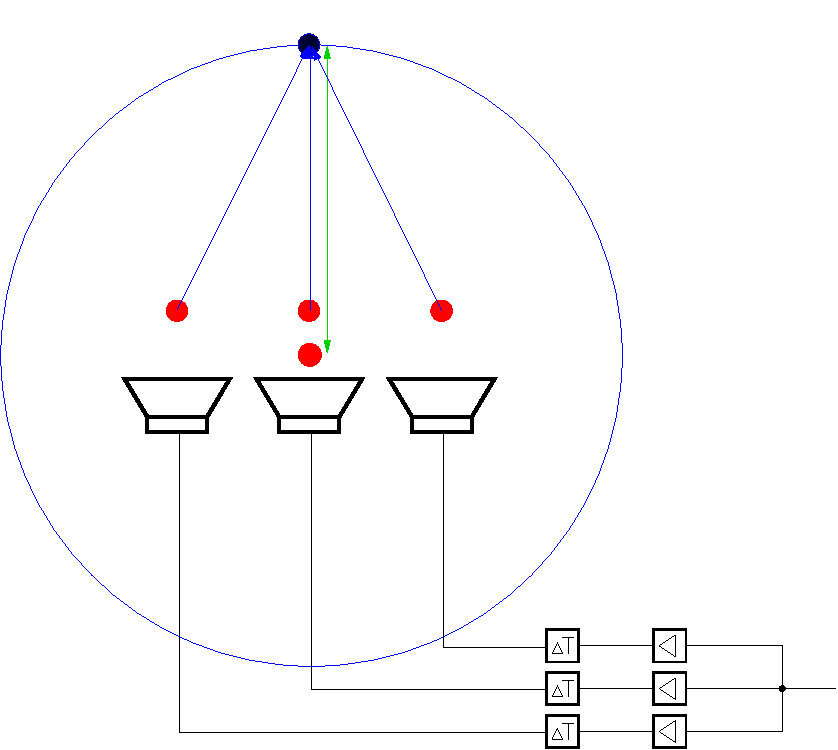
\includegraphics[scale=0.5]{ref_omni_array.pdf}%
\end{picture}%
\setlength{\unitlength}{1658sp}%3315sp}%
%
\begingroup\makeatletter\ifx\SetFigFont\undefined%
\gdef\SetFigFont#1#2#3#4#5{%
  \reset@font\fontsize{#1}{#2pt}%
  \fontfamily{#3}\fontseries{#4}\fontshape{#5}%
  \selectfont}%
\fi\endgroup%
\begin{picture}(7975,7142)(-672,-4729)
\put(1641,-201){\color[rgb]{1,0,0}Ac. Center A}%
\put(5941,-3661){\color[rgb]{0,.56,0}\texttt{Vb}}%
\put(5941,-4066){\color[rgb]{0,.56,0}\texttt{Vb}}%
\put(5941,-4471){\color[rgb]{0,.56,0}\texttt{Vb}}%
\put(4906,-4471){\color[rgb]{0,.56,0}\texttt{0}}%
\put(4906,-4066){\color[rgb]{0,.56,0}\texttt{0}}%
\put(4906,-3661){\color[rgb]{0,.56,0}\texttt{0}}%
\put(2271,2230){\color[rgb]{0,0,0}$L_{p,ref}$}%
\put(2535,219){\color[rgb]{0,.82,0}\SI{10}{\meter}}%
\put(-1409,-201){\color[rgb]{1,0,0}Ac. Center B}%
\put(3936,-651){\color[rgb]{1,0,0}Ac. Center C}%
\put(161,-2106){\color[rgb]{0,0,0}Speaker B}%
\put(1421,-2506){\color[rgb]{0,0,0}Speaker A}%
\put(2681,-2906){\color[rgb]{0,0,0}Speaker C}%
\put(2476,-1051){\color[rgb]{1,0,0}Former array center}%
\end{picture}%
	\caption{Configuration for reference pressure $L_{p,ref}$.}
		\label{fig:ref_omni_array}
\end{figure}
For practical applications, it is preferable to have the same frequency response from the speaker array on the main axis as for the case where no beamforming is executed. In order to achieve this, the input signal has to be sent through a filter with the same amplitude response as the beamforming cost. To avoid nonlinear behaviour from the loudspeakers, it is desirable to keep this equalization to a minimum. Because of this, another minimization criterion has emerged. It can be expressed mathematically as the integral over the beamforming cost.
\subsection{Signal Chain}\label{ssec:sig_chain}
The desired amplitude behaviour of the signals in the loudspeaker array can be achieved by using two filters. First, the signals to all three speakers is run through a filter, that is compensating the beamforming cost. This first filter only has to fulfill certain amplitude specifications, where phase does not matter. Secondly, the signal to the single speaker in the back of the array is run through another filter, that manipulates phase and amplitude according to specifications from \autoref{sec:opt_result} in order to make beamforming happen. The setup is illustrated in \autoref{fig:signal_setup}. Detailed information about the implementation of these filters will be given in \autoref{sec:filter_design}.
\begin{figure}[h]
	\centering
\begin{picture}(0,0)%
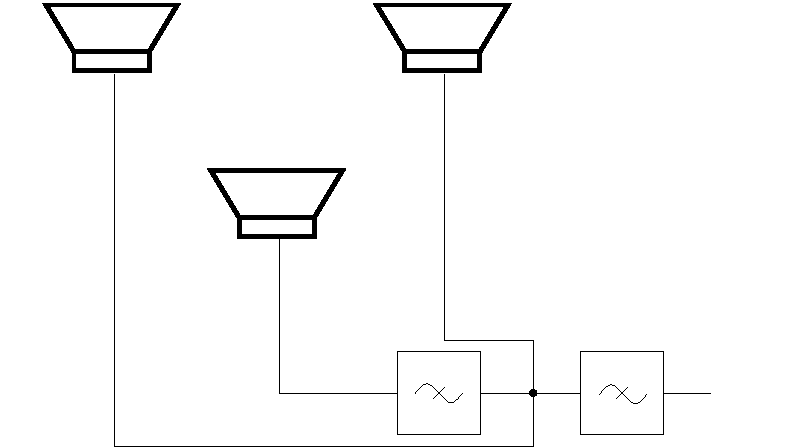
\includegraphics[scale=0.8]{filter_setup.pdf}%
\end{picture}%
\setlength{\unitlength}{3315sp}%4144sp}%
%
\begingroup\makeatletter\ifx\SetFigFont\undefined%
\gdef\SetFigFont#1#2#3#4#5{%
  \reset@font\fontsize{#1}{#2pt}%
  \fontfamily{#3}\fontseries{#4}\fontshape{#5}%
  \selectfont}%
\fi\endgroup%
\begin{picture}(6083,3409)(166,-4573)
\put(41,-1936){Speaker B}%

\put(3646,-1936){Speaker C}%

\put(2386,-3241){Speaker A}%

\put(5311,-4471){Cost Filter}%

\put(1286,-4471){Beamforming Filter}%

\end{picture}%
	\caption{Signal chain for beamforming.}
		\label{fig:signal_setup}
\end{figure}

%The following graph \autoref{fig:graph_plot_three_line} shows the absolute pressure from \SI{60}{\hertz} to \SI{300}{\hertz} of the aligned speaker model. 
%
%\begin{figure}[H]
%	\centering
%	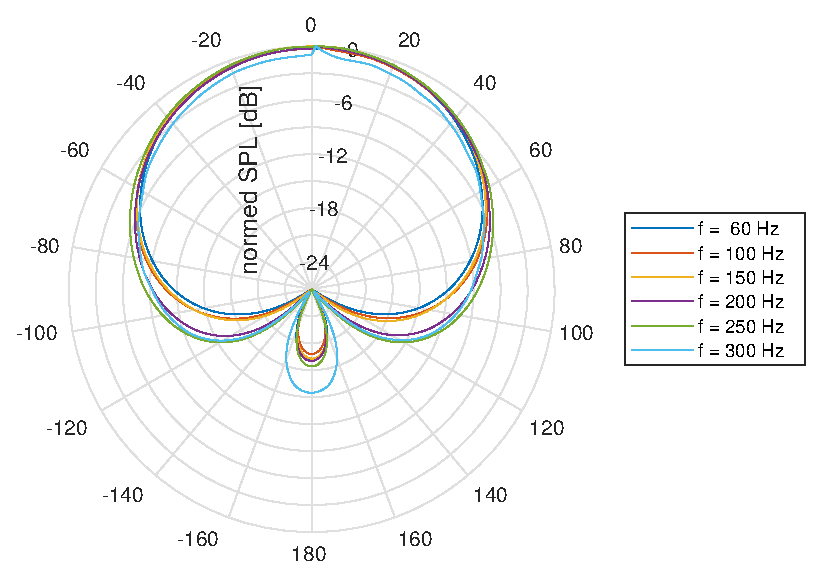
\includegraphics[width=0.7\textwidth]{expected_polar_pcor.eps}
%	\caption{The graph shows the frequency response of the aligned speaker model from \SI{60}{\hertz} to \SI{300}{\hertz}}
%		\label{fig:graph_plot_three_line}
%\end{figure}
\subsection{Settling on a position}\label{ssec:cost_map}
In order to make a a decision on the which parameters \textcolor{green3}{\texttt{Lx}} and \textcolor{green3}{\texttt{Ly}} will be used as fixed values for the final optimization process. The number of feasible solutions is limited by physical constraints when building a reasonable mounting contraption for the array and by the size of the speaker cabinets. It has therefore been decided to assess the beamforming cost via a brute force approach. The beamforming cost has been calculated for every combination of \textcolor{green3}{\texttt{Lx}} and \textcolor{green3}{\texttt{Ly}} in a \SI{5}{\centi\meter} grid. The absolute of the frequency dependent beamforming cost $\Delta L_{p}(f)$ has been intergrated numerically to result in a scalar value, referred to as the cost value. The lowest cost value corresponds to the most ``even" load on the speakers. The results are shown in \autoref{fig:cost_map}.
\begin{figure}[h]
	\centering
	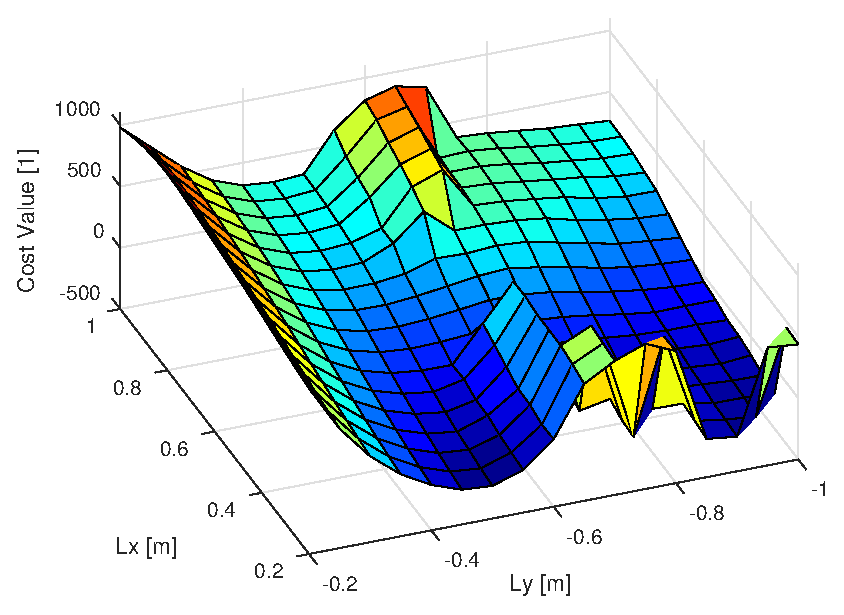
\includegraphics[width=0.7\textwidth]{cost_map.eps}
	\caption{Cost values for feasible acoustical center positions.}
		\label{fig:cost_map}
\end{figure}

\section{Optimization Results}\label{sec:opt_result}
The best genotypes for every frequency can be used to generate polar plots of the expected directional characteristics (\autoref{fig:opt_res_c}). Generating these is done similarly to the fitness evaluation by calculating the normed summed pressure along a circumference using \autoref{eq:aug_omni}.
Because the optimization algorithm has been fixed to a case, where the main axis of the array is orthogonal to the line between two of the acoustic centers, the signal for two of the speakers is the same. The relation between this signal and the signal for the remaining speaker can be plotted for phase and amplitude (\autoref{fig:opt_res_b}). The regressed curves can later be used to find filter parameter (see \autoref{sec:filter_design}).\\
Another plot of the expected directional characteristics is made, based on the regressed parameters, in order to estimate, which effect the filtering will have (\autoref{fig:opt_res_d}).
As mentioned before, in order to achieve this result, the speaker positions parameters \textcolor{green3}{\texttt{Lx}} and \textcolor{green3}{\texttt{Ly}} were fixed.  The beamforming cost is a frequency dependent value that is described in detail in \autoref{sec:main_axis}. For the given optimization, it is plotted in \autoref{fig:opt_res_a}. The results show, that in low frequencies the speaker array emits approx. \SI{6}{\decibel} less pressure than a comparable arrangement of speakers without beamforming. However, towards higher frequencies, the emitted pressure is higher, leading to negative cost values, with a peak around \SI{240}{\hertz} at approx. \SI{-2}{\decibel}. At frequencies higher than that, the graph tends to rise again and displays a value of approx. \SI{-1}{\decibel} at the upper frequency boundary of \SI{300}{\hertz}. It can be noted, that the values, that have been calculated with the augmented source model (\autoref{eq:aug_omni}) only diverge from those that have been calculated with perfectly omnidirectional sources by a negligible quantity.
In order to achieve compatibility with the \gls{fdtd} simulation (see \autoref{sec:fdtd_simulation}), the speaker positioning parameters have to fit within a \SI{5}{\centi\meter} grid. This lead to the decision to investigate the beamforming cost for different positions and to settle on a speaker positioning scheme based on the \SI{5}{\centi\meter}-discreteness and beamforming cost as well as practical considerations about the speaker placement.
\begin{figure}[H]
\begin{subfigure}[c]{0.5\textwidth}
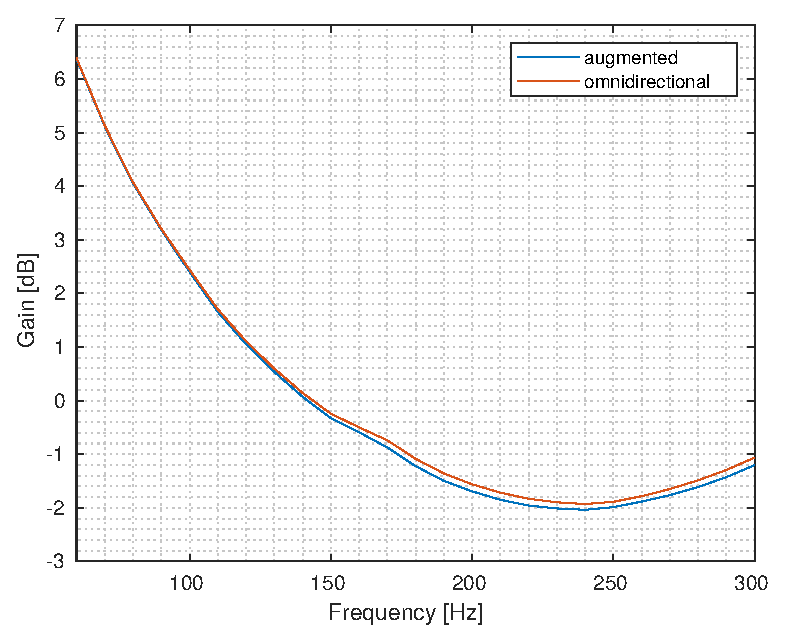
\includegraphics[width=0.85\textwidth]{opt_a.eps}
\subcaption{Beamforming cost}
\label{fig:opt_res_a}
\end{subfigure}
\begin{subfigure}[c]{0.5\textwidth}
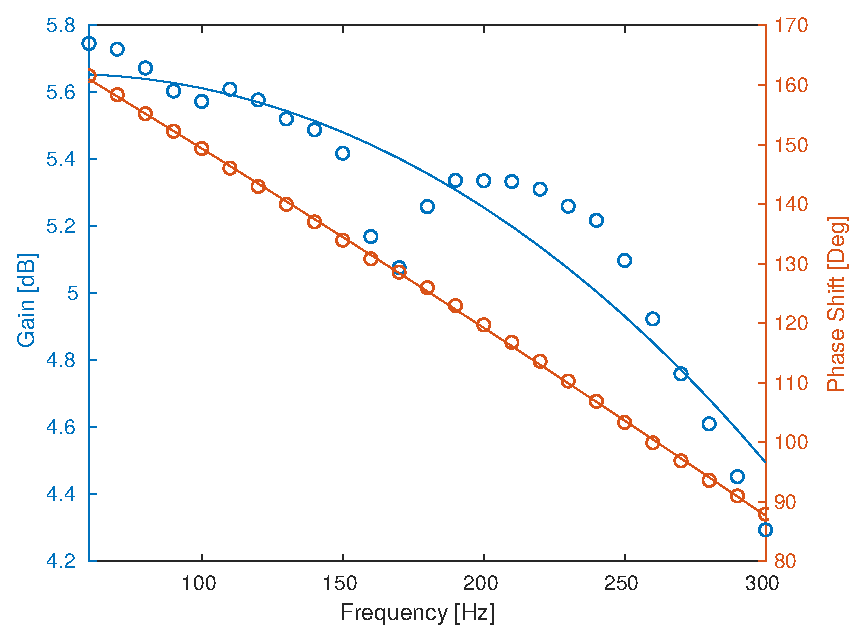
\includegraphics[width=0.95\textwidth]{opt_b.eps}
\subcaption{Beamforming filter requirements}
\label{fig:opt_res_b}
\end{subfigure}\\
\hspace{0.1\textheight}
\begin{subfigure}[c]{0.5\textwidth}
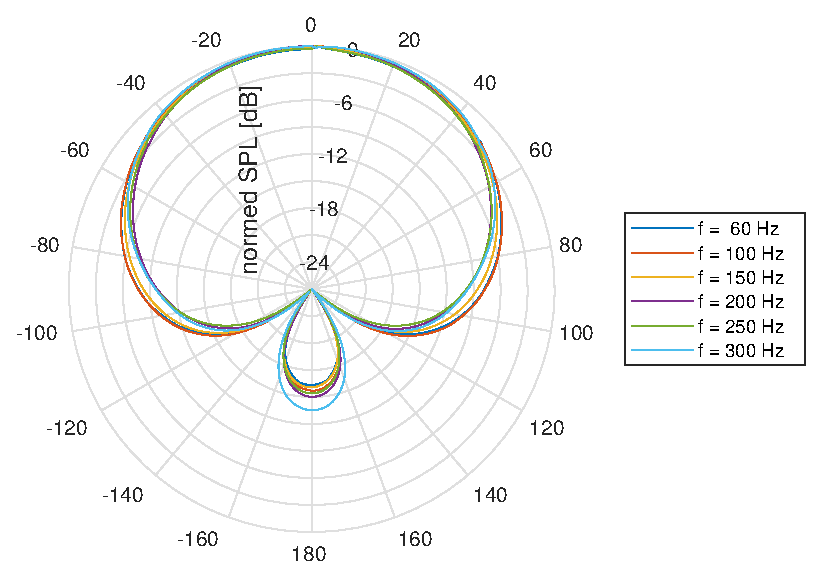
\includegraphics[width=0.95\textwidth]{opt_c.eps}
\subcaption{Directional characteristic, optimal, omnidirectional sources}
\label{fig:opt_res_c}
\end{subfigure}
\begin{subfigure}[c]{0.5\textwidth}
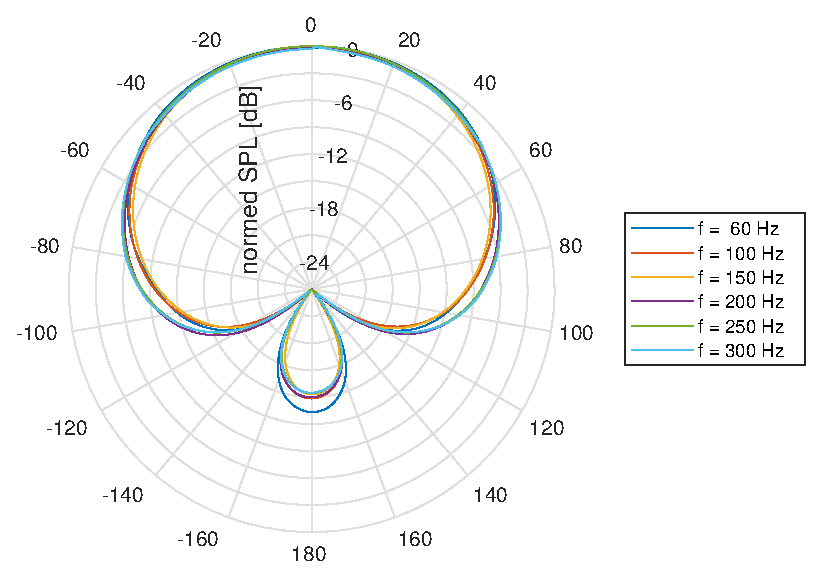
\includegraphics[width=0.95\textwidth]{polar_filtered.eps}
\subcaption{Directional characteristics, filtered, omnidirectional sources}
\label{fig:opt_res_d}
\end{subfigure}\\
\hspace{0.1\textheight}
%\begin{subfigure}[c]{0.5\textwidth}
%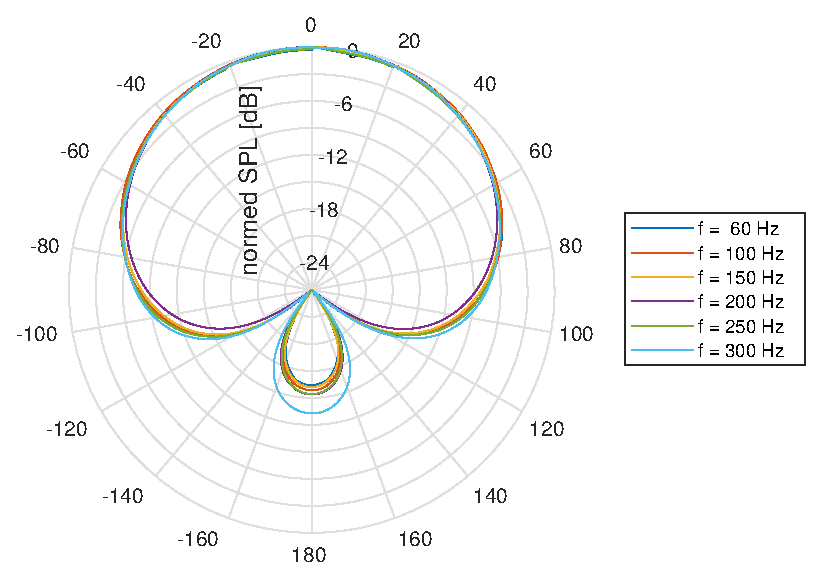
\includegraphics[width=0.95\textwidth]{opt_og_corrected.eps}
%\subcaption{Directional characteristics, optimal, pressure corrected sources}
%\label{fig:opt_res_d}
%\end{subfigure}
%\begin{subfigure}[c]{0.5\textwidth}
%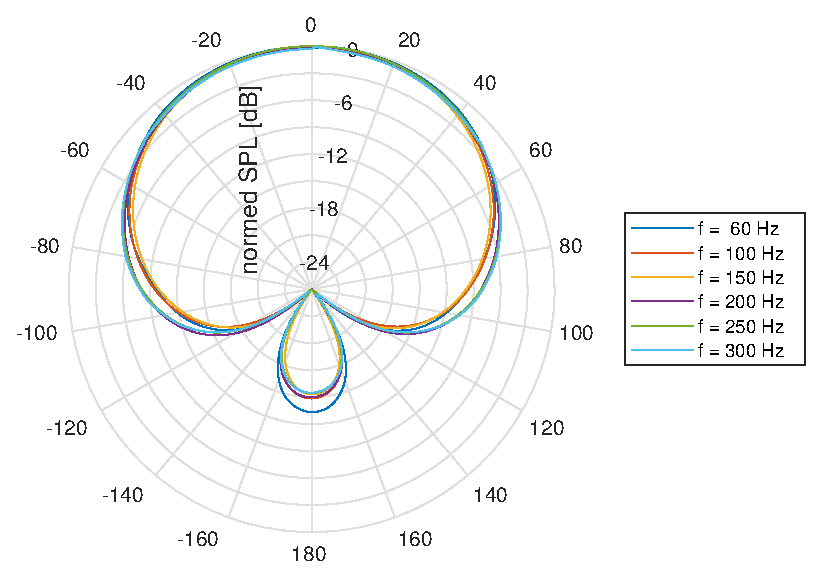
\includegraphics[width=0.95\textwidth]{opt_filter_corrected.eps}
%\subcaption{Directional characteristics, filtered, pressure corrected sources}
%\label{fig:opt_res_d}
%\end{subfigure}\\
\caption{Optimization results, pressure corrected cost function with correction table based on Appendix \ref{ax:directional_2}, \textcolor{green3}{\texttt{Lx}}\,$=$\,\SI{0.4}{\meter}, \textcolor{green3}{\texttt{Ly}}\,$=\,$\SI{-0.4}{\meter}}
		\label{fig:opt_res}
\end{figure}


\section{Conclusion on \gls{sp}-requirements}\label{sec:genetic_con}
The investigations have shown, that at least according to analytical descriptions, the directional characteristics of a triangular loudspeaker array can be shaped in a significant way. The positioning of loudspeakers plays an important role on the signal parameters, that are required. Changing the positions of the loudspeakers will lead to varying results in terms of beamforming cost and directional characteristics. While a main lobe in any direction in relation to the speaker array is technically possible, it has been decided to go with a simplified approach, where the main lobe of the array is perpendicular to a connecting line between two acoustic centers. This leads to a simplified scheme as illustrated in \autoref{fig:signal_setup}, where only two filters are required. The analytical estimates of the directional characteristics of the array will be compared to simulation results that will be obtained with \gls{fdtd} (see. \autoref{sec:fdtd_simulation}. Finally, an implementation of the filters will be executed and polar response measurements will be performed. 		
	\chapter{Filter Development}
	\section{Filter}\label{sec:filter_design}

The aim of this chapter is to analyse the data from \ref{sec:opt_result} and choose the implementation method. From the beam forming optimization \autoref{sec:genetic_con} it was concluded that there shall be a cost filter and a beam forming filter. This chapter starts analyse the cost filter and design a filter solution, then the beam forming filter will be analysed and a solution will be designed.


\section{The cost filter}
The analysis of the cost filter will be done only with respect to the gain of the transfer function and without taking the phase intro account. The reason to avoid the phase is that the filter is an input filter to the entire system, and therefore the phase of the filter will affect all speaker the same way and therefore not effect the beam forming. \\
To analyse the cost filter, the filter type and the slope or Q of the filter have to be determined. 

the filter type will be determined first. To determined the filter type, a second order polynomia estimation will be done on the data point of the cost filter. The polynomia estimation is done with MATLAB command \texttt{polyfit()} with a second order regression. This give a second order polinomia where  \texttt{polyval()} is used to estimate the filter transfer function. The estimation will be done from \SI{60}{\hertz} to \SI{400}{\hertz}. The \SI{400}{\hertz} choice is made such that the estimation fit at lest to the double frequency of beam forming interest. The following \autoref{} shows the estimate compare to the original data point.

\begin{figure}[H]
	\centering
	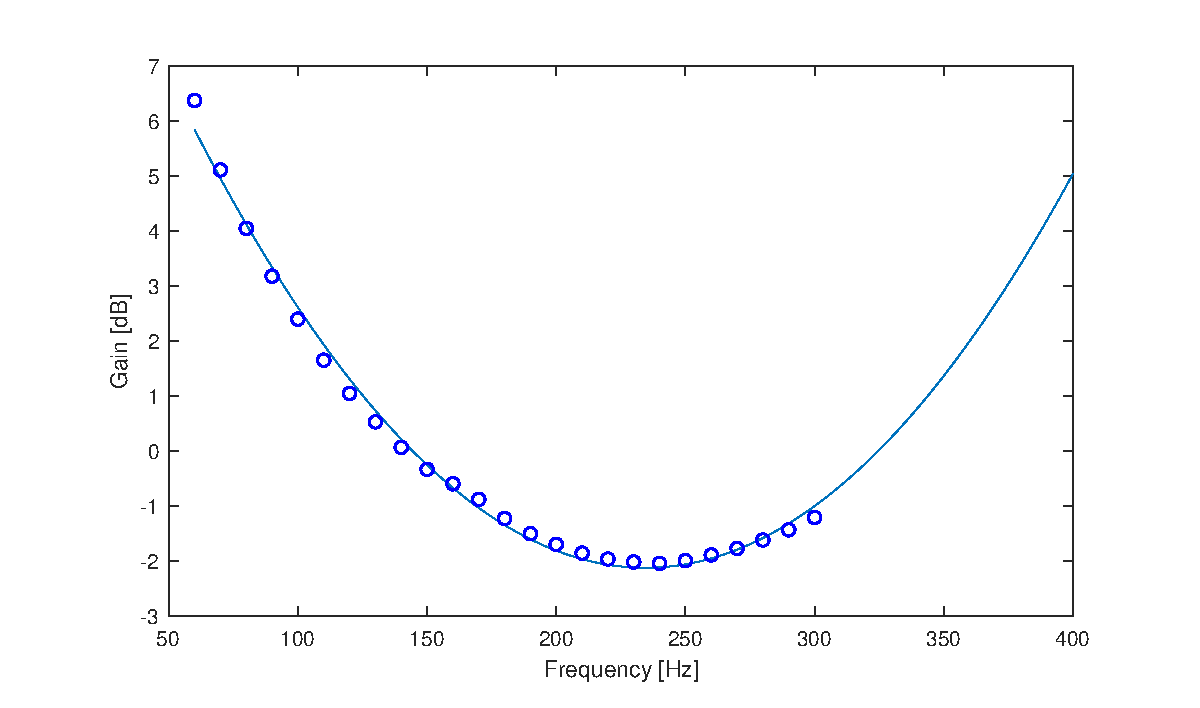
\includegraphics[width=1\textwidth]{band_stop_filter.eps}
	\caption{The graph shows transfer function of the estimated transfer function, where the blue  Solid line is the gain. All circle in the graph is the actual optimized point.}
		\label{fig:band_stop_filter}
\end{figure}
It can also be seen on \autoref{band_stop_filter} the shape of the estimated cost filter is a band stop filter. \\

\subsection{Parametric equalizer as cost filter}

Designing a bandstop filter is done with designing it as a bandpass filter, and use it in a feedback circuit. The following block diagram \autoref{fig:bandstop_filter_blockdiagram} shows a block diagram of a bandstop filter. 

\begin{figure}[H]
	\centering
\begin{picture}(0,0)%
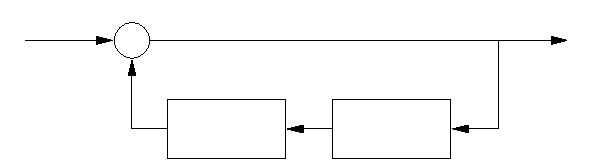
\includegraphics{bandstop_filter_blockdiagram.pdf}%
\end{picture}%
\setlength{\unitlength}{4144sp}%
%
\begingroup\makeatletter\ifx\SetFigFont\undefined%
\gdef\SetFigFont#1#2#3#4#5{%
  \reset@font\fontsize{#1}{#2pt}%
  \fontfamily{#3}\fontseries{#4}\fontshape{#5}%
  \selectfont}%
\fi\endgroup%
\begin{picture}(4634,1218)(2056,-973)
\put(2071, 74){Input}%
\put(3196,-376){-}%
\put(3556,-781){Gain}%
\put(4681,-781){Bandpass}%
\put(2791,-286){+}%
\put(6076, 74){Output}%
\end{picture}%
	\caption{The figure shows the block diagram of a bandstop filter}
		\label{fig:bandstop_filter_blockdiagram}
\end{figure}


Designing the bandpass filter part of the bandstop filter, the bandpass filter part is changed such that the center frequency is at \SI{0}{\decibel} and the shape is a bandpass filter and not a bandstop filter. To change the filter, the parameter is inverter and subtracted \SI{2.1}{\decibel}. The following \autoref{fig:band_pass_filter} shows the bandpass filter.

\begin{figure}[H]
	\centering
	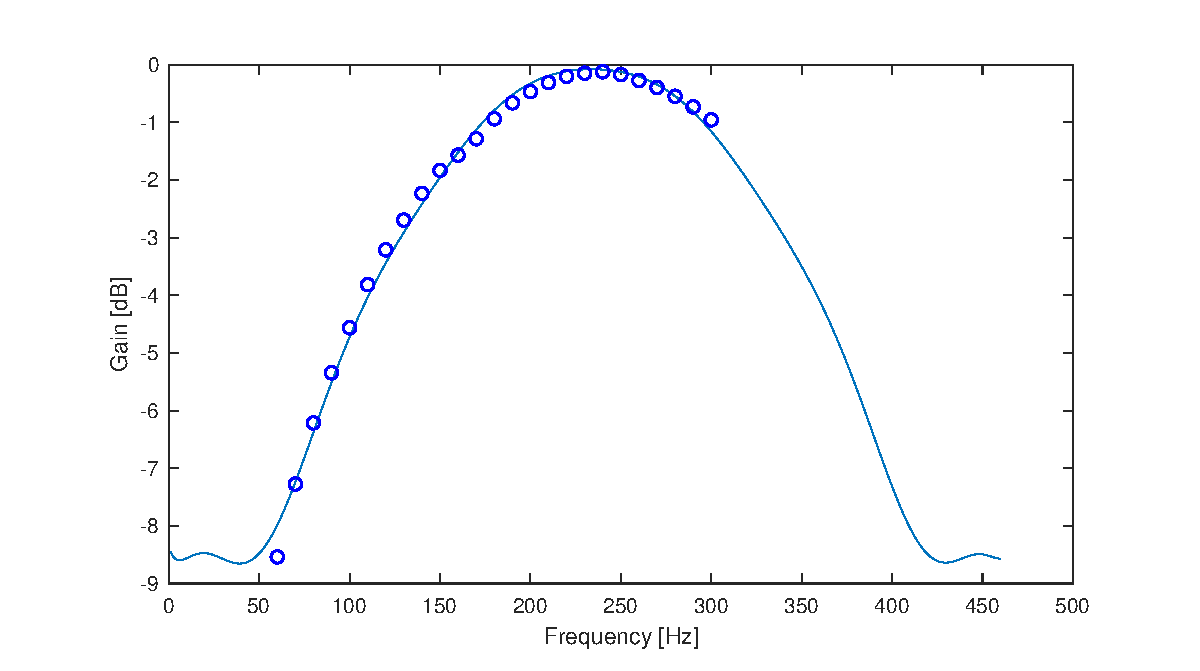
\includegraphics[width=1\textwidth]{band_pass_filter.eps}
	\caption{The graph shows transfer function of the estimated transfer function, where the blue  Solid line is the gain. All circle in the graph is the actual optimized point.}
		\label{fig:band_pass_filter}
\end{figure}

On \autoref{fig:band_pass_filter} it can be seen that the \SI{-3}{\decibel} bandwidth is \SI{213}{\hertz} with a relative gain of \SI{8.5}{\decibel}, and have a center frequency of \SI{234}{\hertz}. There needs to be a gain factor before the filter, to achieve the wanted band stop filter. and the gain will need to be \SI{6.4}{\decibel}.. The initial filter parameters is then:

\begin{itemize}
\item Gain $G = \SI{8.5}{\decibel}$
\item Bandwidth is $BW = 2\pi \SI{213}{\hertz} = 1338.3$
\item Center frequency is $\omega_0 = 2\pi \SI{234}{\hertz} = 1470.3$
\item The filter goodness $Q = \frac{1470.3}{1338.3} = 1.0986$
\end{itemize}

The corresponding transfer function to block diagram \autoref{fig:bandstop_filter_blockdiagram} is as \autoref{eq:bandstop_filter_eq}

\begin{equation}\label{eq:bandstop_filter_eq}
H_{stop}(s) = \frac{s^2+\frac{\omega_0}{Q}s+\omega_0^2}{s^2+\frac{\omega_0}{Q}s(1+Gain)+\omega_0^2}
\end{equation}

A bode plot of the \autoref{eq:bandstop_filter_eq} is showen in \autoref{fig:bandstop_filter_eq_bodeplot}



\begin{figure}[H]
	\centering
	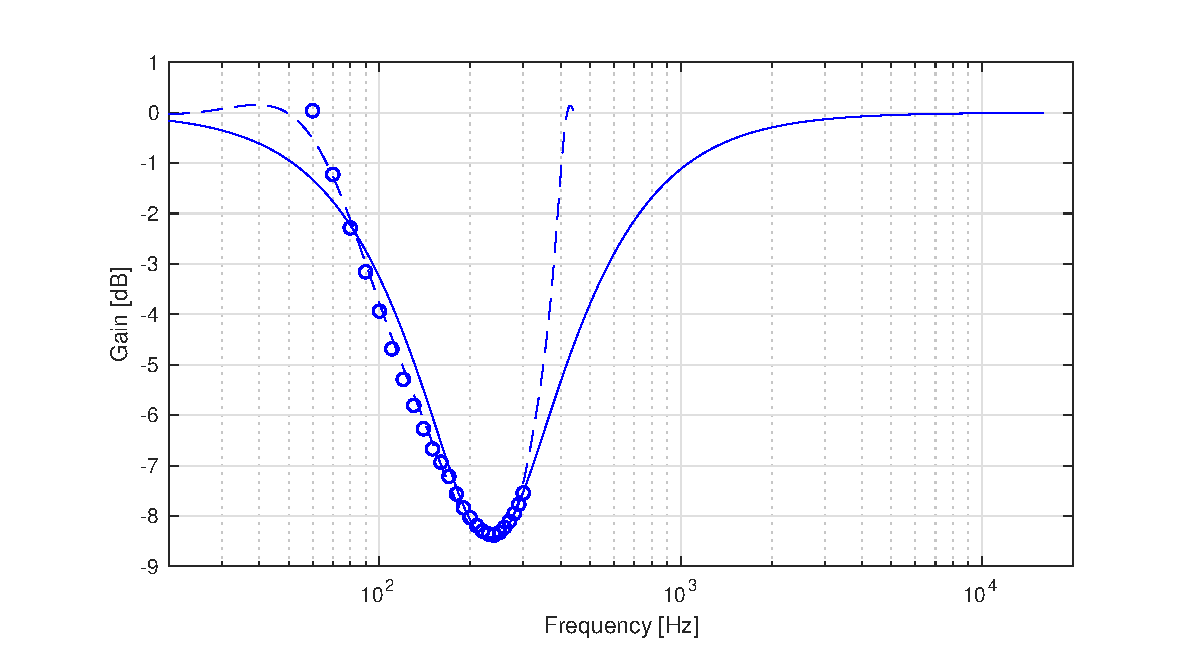
\includegraphics[width=1\textwidth]{bandstop_filter_eq_bodeplot.eps}
	\caption{The figure shows the bode plot of the \autoref{{eq:bandstop_filter_eq}}}
		\label{fig:bandstop_filter_eq_bodeplot}
\end{figure}

On the bode plot  \autoref{fig:bandstop_filter_eq_bodeplot} the filter parameter fits very well from \SI{80}{\hertz} and upwards but the frequency that is below \SI{80}{\hertz} is to fare off. To solve this problem, the data point can be atenuated to fit on the steap slop of the filter. 


As it can be seen on \autoref{fig:bandstop_filter_eq_bodeplot} the parameter have to be changed a bit to fit the data point. By tryil and error the following filter parameters have been selected for the cost filter. 

\begin{itemize}
\item Gain $G = \SI{7.2}{\decibel}$
\item Bandwidth is $BW = 2\pi \SI{253}{\hertz} = 1589.6$
\item Center frequency is $\omega_0 = 2\pi \SI{234}{\hertz} = 1470.3$
\item The filter goodness $Q = \frac{1470.3}{1338.3} = 0.9249$
\end{itemize}


The wanted filter is raised by \SI{2}{\decibel} such that the designed filter also fit at low frequency. The output of the filter shall afterwards by atunuated by  \SI{2}{\decibel} to work as wanted.


It can be seen on \autoref{fig:band_pass_filter_h_non_scaled} that the \SI{-3}{\decibel} bandwidth is to narrov because the wanted filter have symmetrical shape in linear domain and not in logorithmic doman which the filter have.Therefore the filter bandwidth have to be extended with a factor of 1.1878. The factor is founded by trail and error. After the bandwidth is extended the filter is as following \autoref{fig:band_pass_filter_h}


\begin{figure}[H]
	\centering
	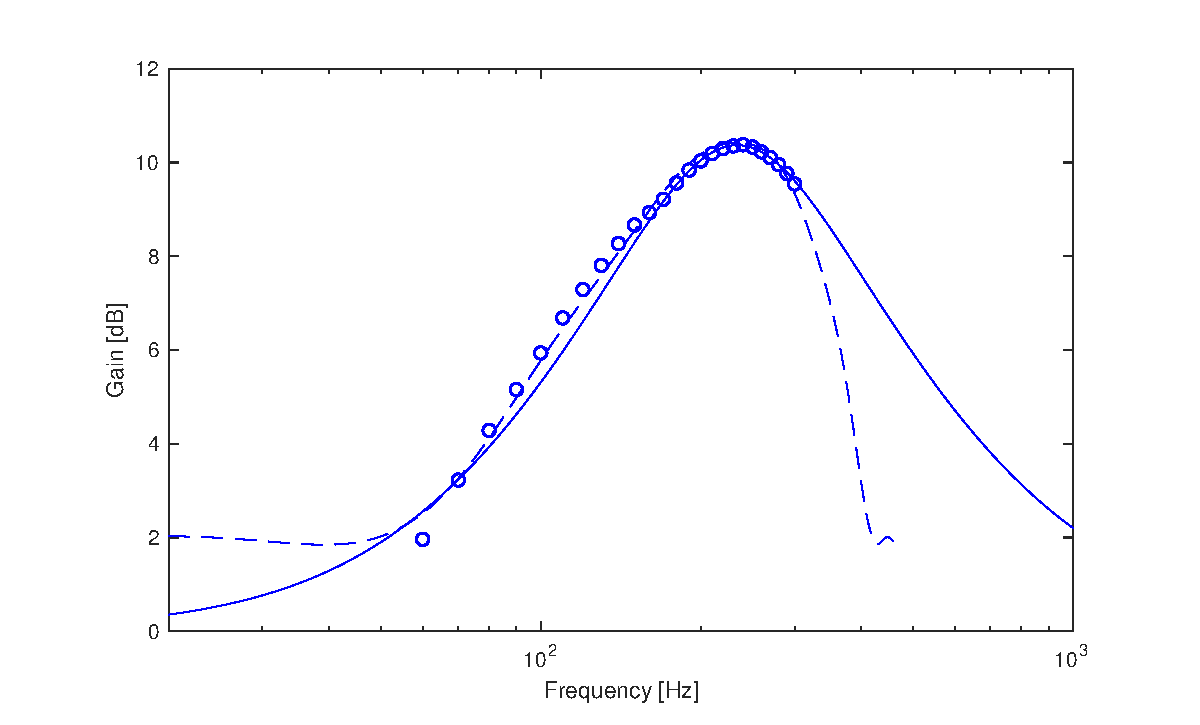
\includegraphics[width=1\textwidth]{band_pass_filter_h.eps}
	\caption{The graph shows transfer function of the estimated transfer function, where the blue  Solid line is the gain. All circle in the graph is the actual optimized point.}
		\label{fig:band_pass_filter_h}
\end{figure}


\subsection{Band stop filter form second order filter}
To transform a band pass filter to a band stop filter which not is a notch filter, the filter have to be transformed from a feed forward filter to a feedback filter 


(BLOCK DIAGRAM)

To transform the bandpass filter to a bandstop filter as descriped above, only the denominator and the numerator have to be switch around.

(The new formula)


\begin{figure}[H]
	\centering
	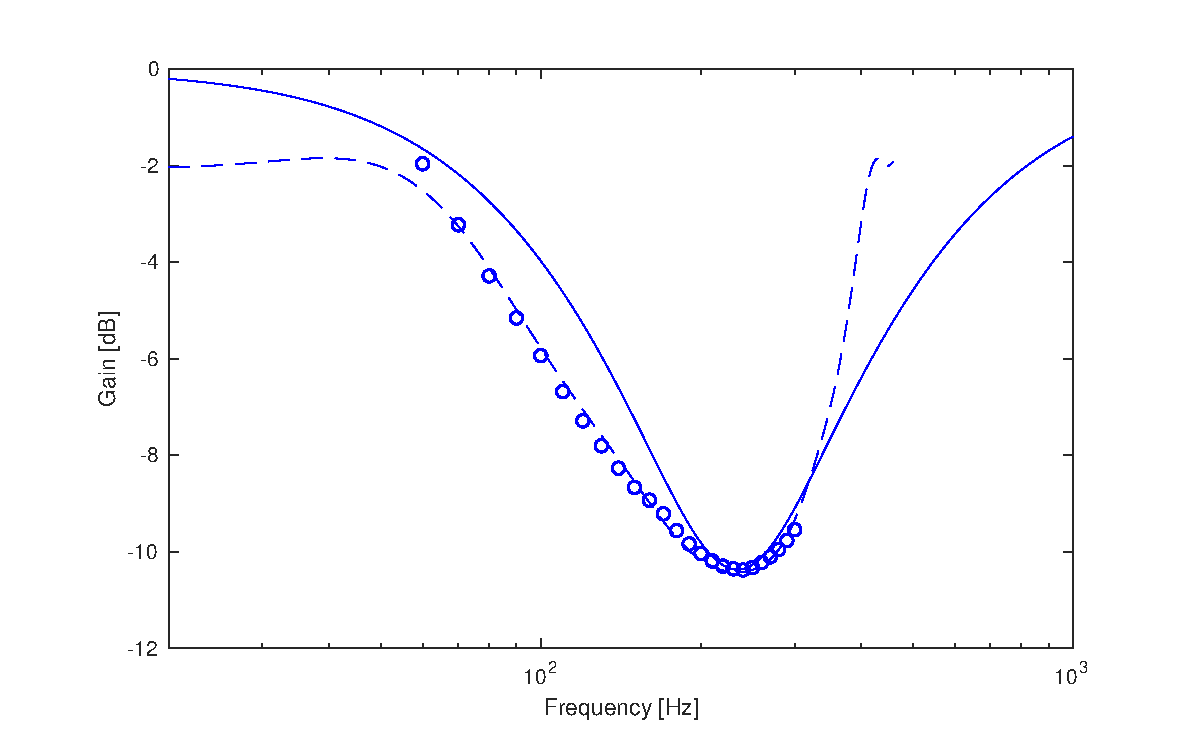
\includegraphics[width=1\textwidth]{band_stop_filter_non_scaled.eps}
	\caption{The graph shows transfer function of the estimated transfer function, where the blue  Solid line is the gain. All circle in the graph is the actual optimized point.}
		\label{fig:band_stop_filter_non_scaled}
\end{figure}


\begin{figure}[H]
	\centering
	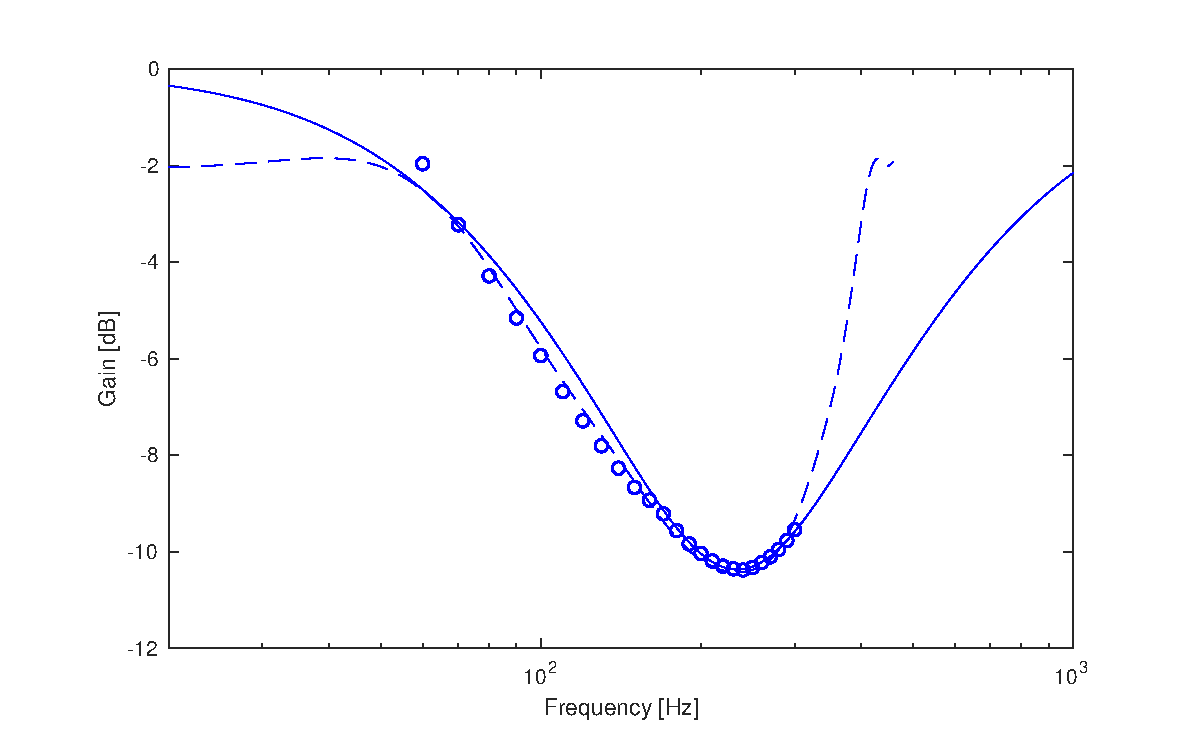
\includegraphics[width=1\textwidth]{band_stop_filter_scaled.eps}
	\caption{The graph shows transfer function of the estimated transfer function, where the blue  Solid line is the gain. All circle in the graph is the actual optimized point.}
		\label{fig:band_stop_filter_scaled}
\end{figure}


 The second step is to find the slope of the needed low pass filter. The slope is founded as following \autoref{eq:filter_slope}

\begin{equation}
\text{slope} = \frac{G_2\si{\decibel}-G_1\si{\decibel}}{\log_{10}{(f_2)}-\log_{10}{(f_1)}}
\end{equation}

    \startexplain
    \explain{$f$ is a frequency point }{\si{\hertz}}
    		\explain{$f_2$ is a frequency point higher that $f_1$ }{\si{\meter}}
        \explain{$G_1\si{\decibel}$ is the corresponding amplitude to $f_1$}{\si{\decibel}}
         \explain{$G_2\si{\decibel}$ is the corresponding amplitude to $f_2$}{\si{\decibel}}
    \stopexplain
    
The calculated slope is $17 \frac{\si{\decibel}}{dec}$ and it have been chosen that a standard first order low pass filter will be used. The following \autoref{} shows the error between the data and the filter. The error will make a pressure deference, that defence on frequency. 


\section{Beam forming filter}
The beam forming filter is not as easy as the cost filter to design, since that the phase and the gain have to be exact before the beam forming works. Therefore the phase have to be studied to determined the filter type. On the data point from the \ref{sec:opt_result} it can be seen that the phase is mostly linear in the frequency of interest, and therefore the filter will be a linear phase \gls{fir} filter. The smart thing with choosing a \gls{fir} filter is that the impulse response of the filter just have to be symmetric to achieve linear phase response. This means that optimizing the part of the impulse response and put it together with a mirrored version will always achieve linear phase. One disadvantages is that the cut off frequency is in the low frequency and therefore the filter order have to be high. \\

 A modified version of the genetic optimization algorithm will be used to find a optimized impulse response of the filter. To optimize the impulse respond of the filter, an estimate of the impulse respond have to be determined. One and the used way to estimate the impulse response is to transfer all polar coordinate to a complex rectangular transfer function and take the real of the \gls{ifft} of the complex transfer function. The polar to rectangular transform is done as following \autoref{eq:pol_to_regt}

\begin{equation}\label{eq:pol_to_regt}
x=rcos(\phi)+j \cdot rsin(\phi)
\end{equation}


     \startexplain
    \explain{$\phi$ is the angle of the transfer function in radian }{\si{1}}
        \explain{$r$ is the amplitude of the transfer function}{\si{1}}
        \explain{$j$ is the imaginary unit}{\si{1}}
    \stopexplain

The real of the \gls{ifft} gives an estimated impulse response but with a scaled cross over point. The meaning with scaled cross over point is that the cross over point follows the scaling of the sample frequency. With a sample rate of \SI{44.1}{\kilo\hertz} the following  \autoref{} shows the transfer function of the estimated impulse response. 

\begin{figure}[H]
	\centering
	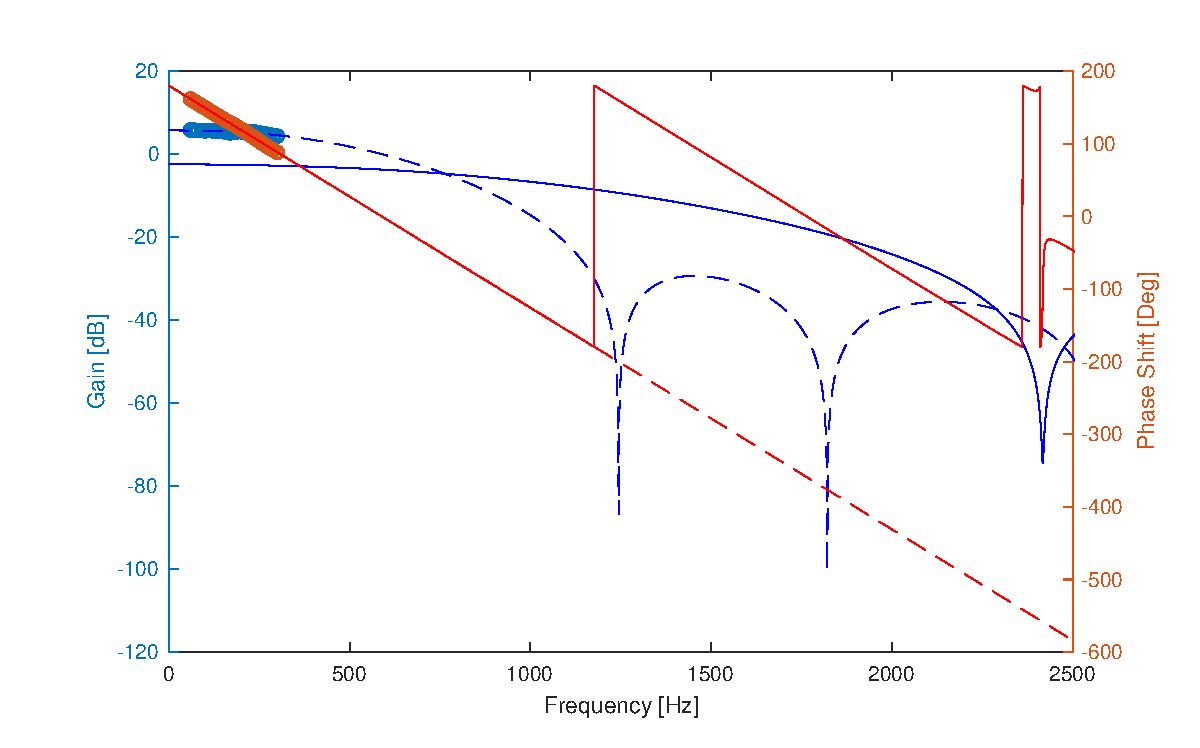
\includegraphics[width=1\textwidth]{ir_estimate_non_scaled.eps}
	\caption{The graph shows transfer function of the estimated impulse respond. The dashed line is transfer function that is needed for beam forming filter, where the blue line is the gain and the red line is the phase. The Solid line line is the transfer function of the estimated impulse response, where the blue line is the gain and the red line is the phase. All circle in the start of the graph is the actual optimized point.}
		\label{fig:ir_estimate_non_scaled}
\end{figure}


It can be seen that the cross over lays at a too high frequency and the gain at the frequency of interest is to low. The corresponding impulse response of the transfer function in \autoref{fig:ir_estimate_non_scaled} is as following \autoref{fig:ir_estimate_non_mirror} where the mirrored version not is added yet. 

\begin{figure}[H]
	\centering
	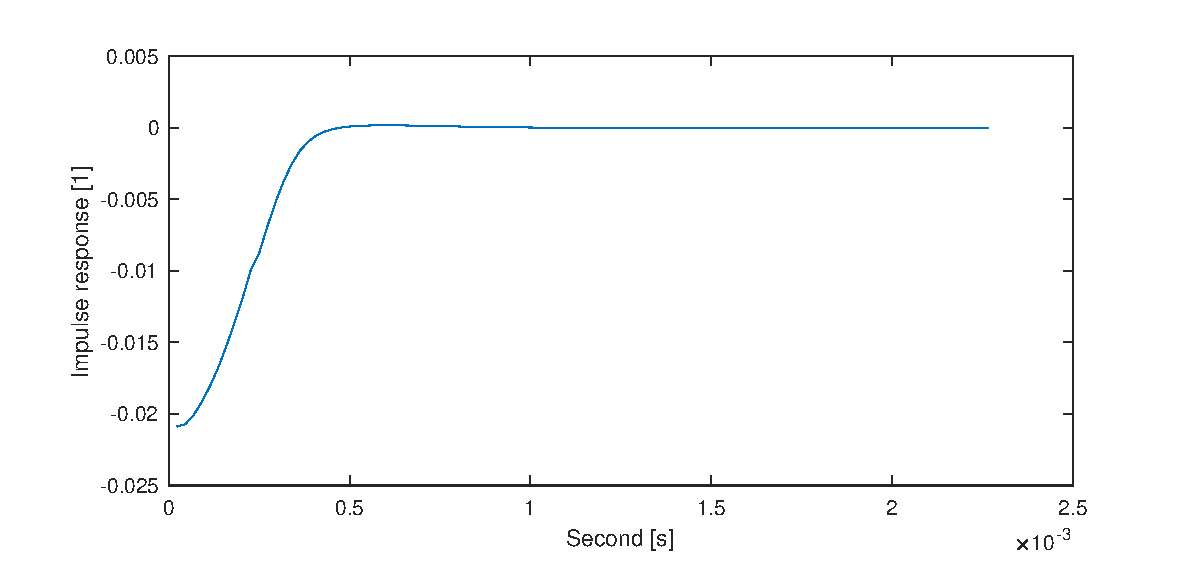
\includegraphics[width=1\textwidth]{ir_estimate_non_mirror.eps}
	\caption{The graph shows the impulse respond where the mirrored version is added to the impulse respond}
		\label{fig:ir_estimate_non_mirror}
\end{figure}

The version where the mirrored impulse response is added to the impulse response and the phase is matched to the wanted phase and is the corresponding impulse response to \autoref{fig:ir_estimate_non_scaled} is \autoref{fig:ir_estimate_mirror}

\begin{figure}[H]
	\centering
	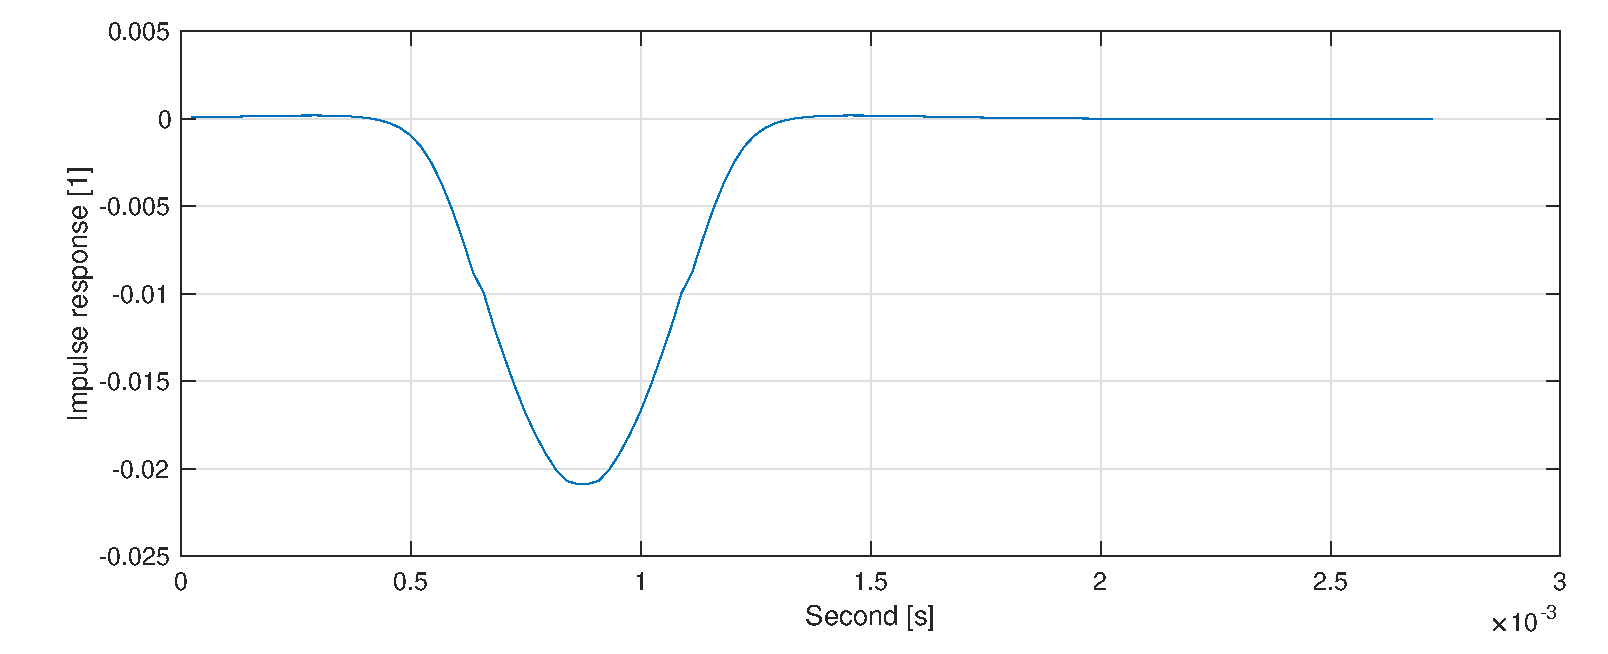
\includegraphics[width=1\textwidth]{ir_estimate_mirror.eps}
	\caption{The graph shows the impulse respond where the mirrored version is added to the impulse respond}
		\label{fig:ir_estimate_mirror}
\end{figure}


The impulse response have to be change the right way to make a good estimate. The way to lower the cross over point is to extend the part of the impulse respond that it have the highest amplitude, which also make the impulse response longer. Thinking about the theory of the \gls{fir} filter, that the lower cross over, the higher order the filter have to be and therefore the impulse respond gets longer. The following \autoref{} shows the estimated impulse respond that will be used for the optimization, where the crossover is approximatly where it shall be. 


\begin{figure}[H]
	\centering
	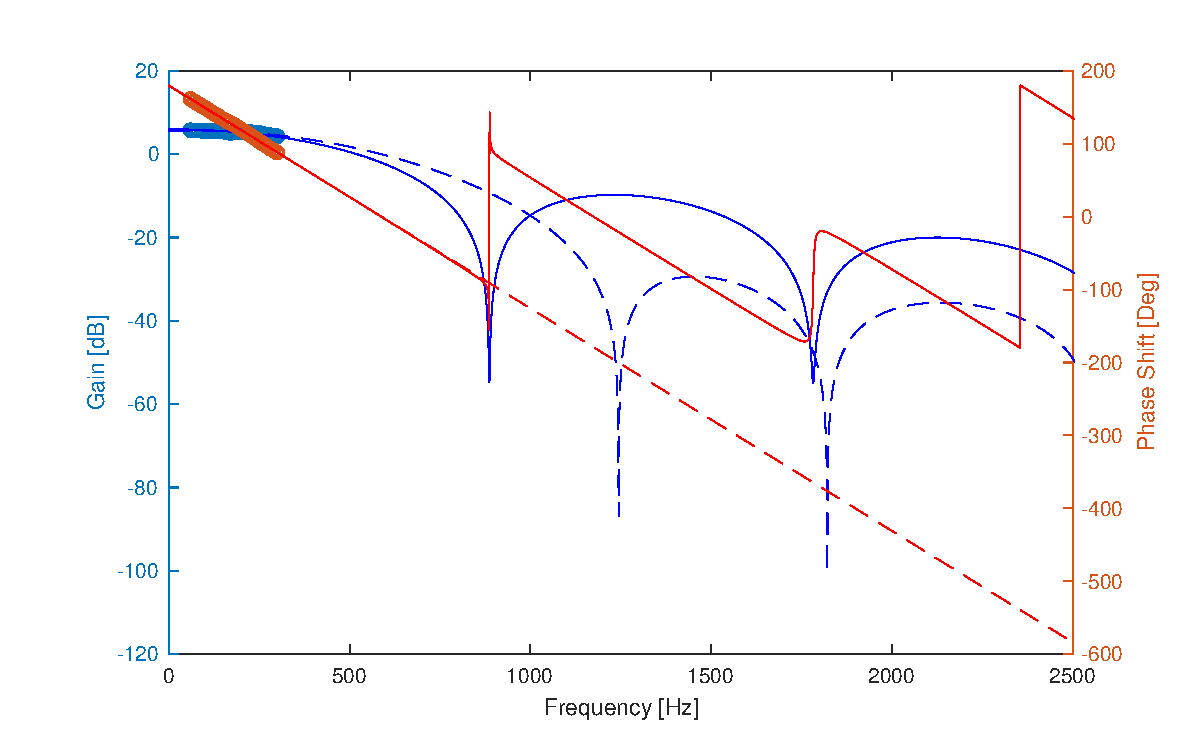
\includegraphics[width=1\textwidth]{ir_estimate_scaled.eps}
	\caption{The graph shows transfer function of the estimated impulse respond. The dashed line is transfer function that is needed for beam forming filter, where the blue line is the gain and the red line is the phase. The Solid line line is the transfer function of the estimated impulse response, where the blue line is the gain and the red line is the phase. All circle in the start of the graph is the actual optimized point.}
		\label{fig:ir_estimate_scaled}
\end{figure}


\begin{figure}[H]
	\centering
	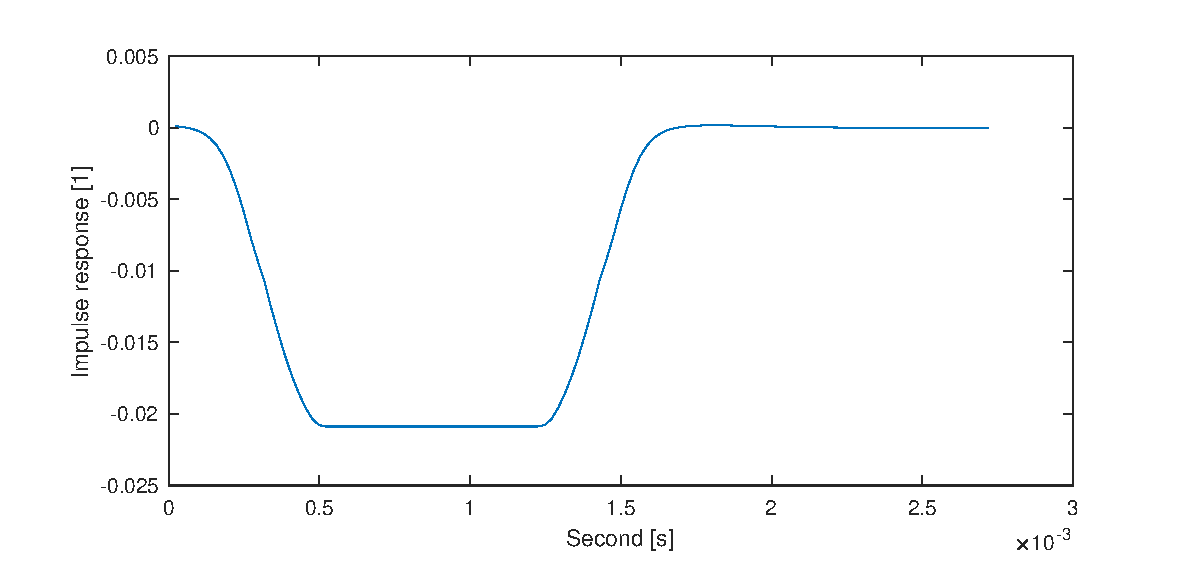
\includegraphics[width=1\textwidth]{ir_estimate_mirror_scale.eps}
	\caption{The graph shows the impulse respond where the mirrored version is added to the impulse respond}
		\label{fig:ir_estimate_mirror_scale}
\end{figure}

Where the corresponding impulse response is as \autoref{fig:ir_estimate_mirror_scale}

\begin{figure}[H]
	\centering
	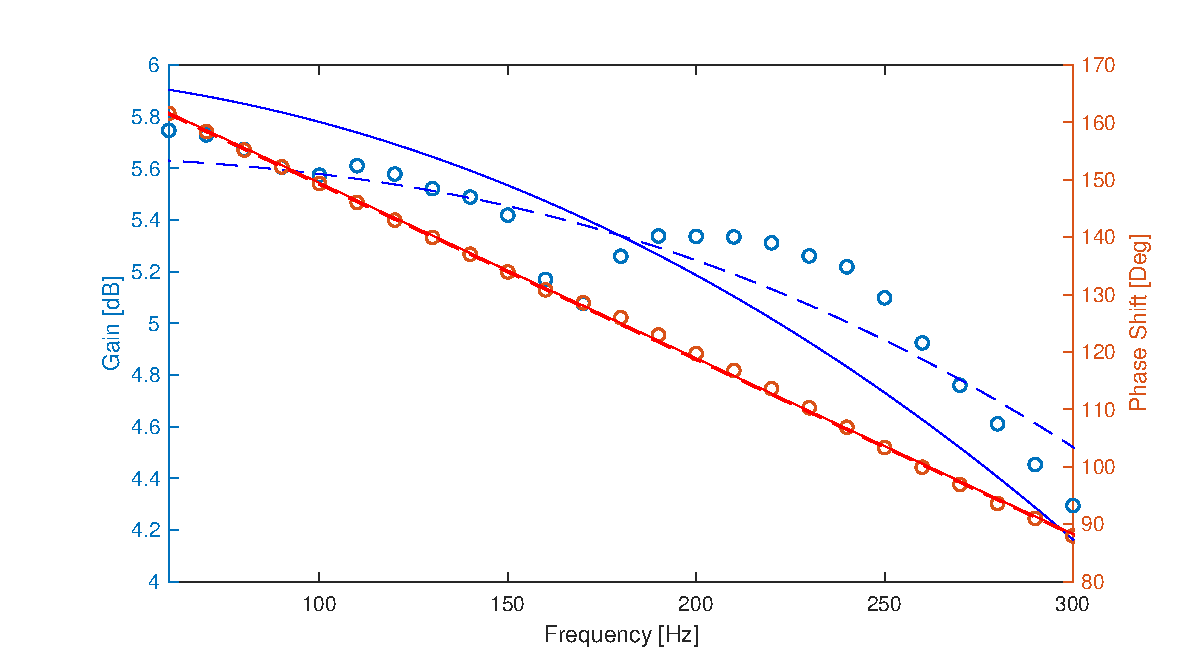
\includegraphics[width=1\textwidth]{ir_estimate_scaled_close.eps}
	\caption{The graph shows transfer function of the estimated impulse respond. The dashed line is transfer function that is needed for beam forming filter, where the blue line is the gain and the red line is the phase. The Solid line line is the transfer function of the estimated impulse response, where the blue line is the gain and the red line is the phase. All circle is the actual optimized point.}
		\label{fig:ir_estimate_scaled_close}
\end{figure}

As it can be seen at \autoref{fig:ir_estimate_scaled} that the cut off is lowered and the gain is automatic raised to the wanted area. A closer look on the area of the frequency of interest in 

It can be seen at \autoref{ir_estimate_scaled_close} that the fit is close, but the gain can be optimized. Recalling from earlier, a linear phase \gls{fir} filter have to have symmetric impulse response and therefore the impulse respond where the mirrored version is not added will be used as initial guess for the genetic optimizer. To optimize the impulse response there will be used high probability for mutation and crossover. The resend to use high probability for mutation, is that the shape of the impulse response is changed a bit for every mutation, and it is the shape there needs to be change to get the optimized \gls{fir} filter coefficient. In the mutation part, the following mutation is done.

\begin{itemize}
\item One single random chosen point in the impulse response is change by moving it up and down wards.
\item One random chosen area of the impulse response is change by moving it up and down wards with a Gaussian shape, where $\mu$ and $\sigma$ is random chosen.
\item An up-sampling is done on the impulse respond with a factor of ten. After the up-sampling the value at time zero is copied and used ans the new zero point after the impulse response is shifted one sample to the right. The resend to up-sample is that the shift only is one tenth. This technique do that the cost can be minimized more than without up-sampling. The up-sampling is done with linear interpolation. This mutation ends with a down sampling with a factor of ten such that the impulse respond is at the same length as at the start.
\item There is one mutation that only multiply a factor to the impulse respond. 
\end{itemize}

At the end of all mutation the last point of the impulse response is used as the \gls{dc} offset and the offset will be subtracted from the impulse response , such that the impulse response end at an amplitude of zero. 

\section{Result}


 

\begin{figure}[H]
	\centering
	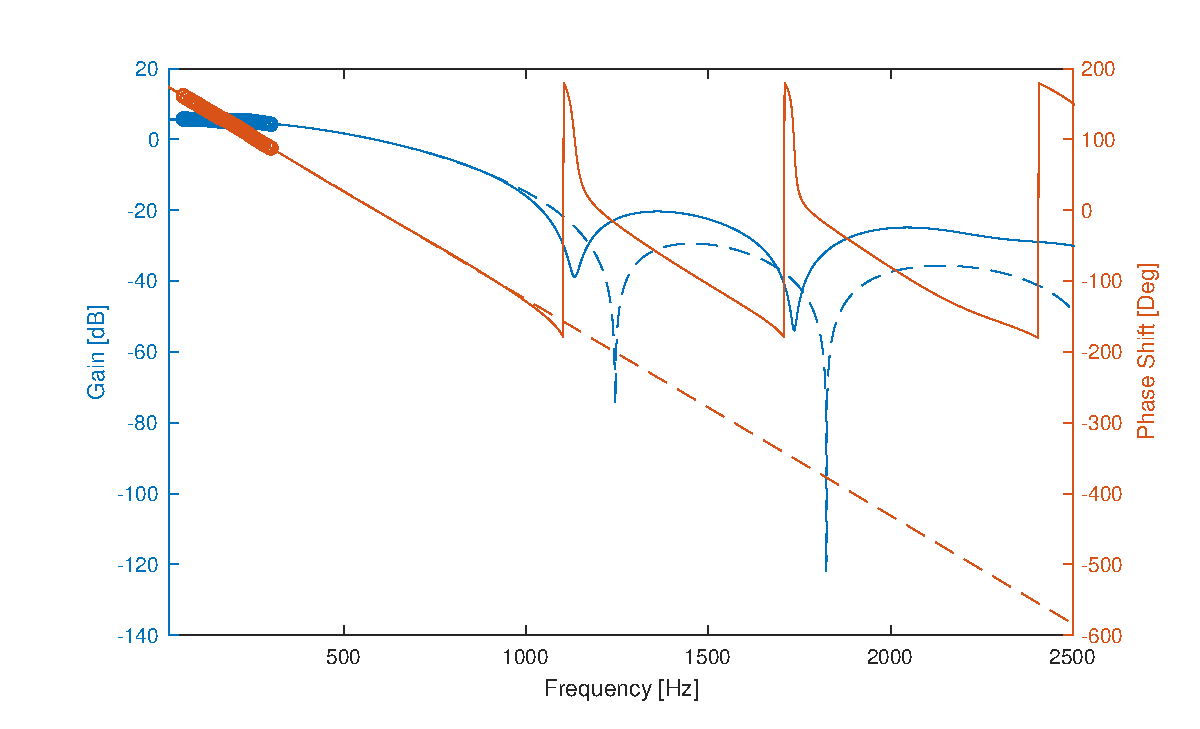
\includegraphics[width=1\textwidth]{filter_vs_reg.eps}
	\caption{The graph shows transfer function of the estimated impulse respond. The dashed line is transfer function that is needed for beam forming filter, where the blue line is the gain and the red line is the phase. The Solid line line is the transfer function of the estimated impulse response, where the blue line is the gain and the red line is the phase. All circle in the start of the graph is the actual optimized point.}
		\label{fig:filter_vs_reg}
\end{figure}

\begin{figure}[H]
	\centering
	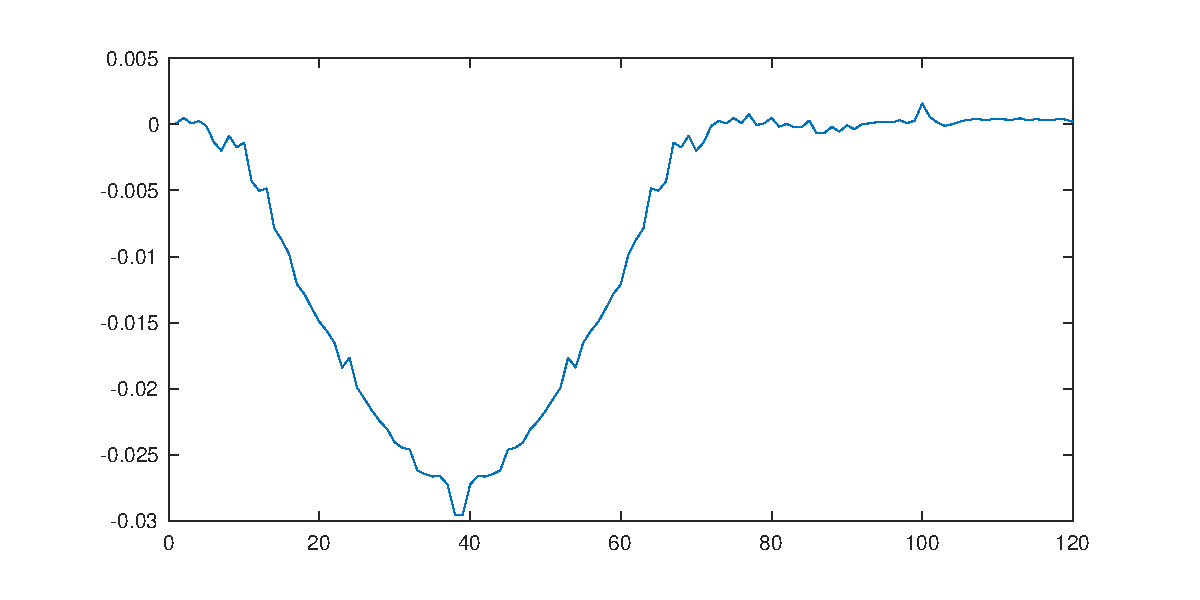
\includegraphics[width=1\textwidth]{filter_coefficient.eps}
	\caption{The graph shows the impulse respond where the mirrored version is added to the impulse respond}
		\label{fig:filter_coefficient}
\end{figure}

As it can be seen at \autoref{fig:ir_estimate_scaled} that the cut off is lowered and the gain is automatic raised to the wanted area. A closer look on the area of the frequency of interest in 


\begin{figure}[H]
\begin{subfigure}[c]{0.5\textwidth}
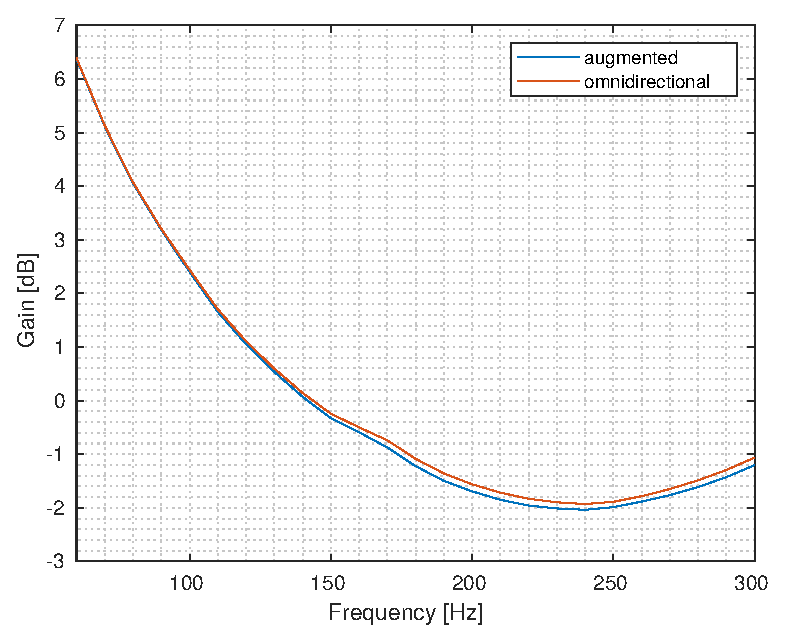
\includegraphics[width=0.85\textwidth]{opt_a.eps}
\subcaption{cost filter}
\label{fig:opt_res_a}
\end{subfigure}
\begin{subfigure}[c]{0.5\textwidth}
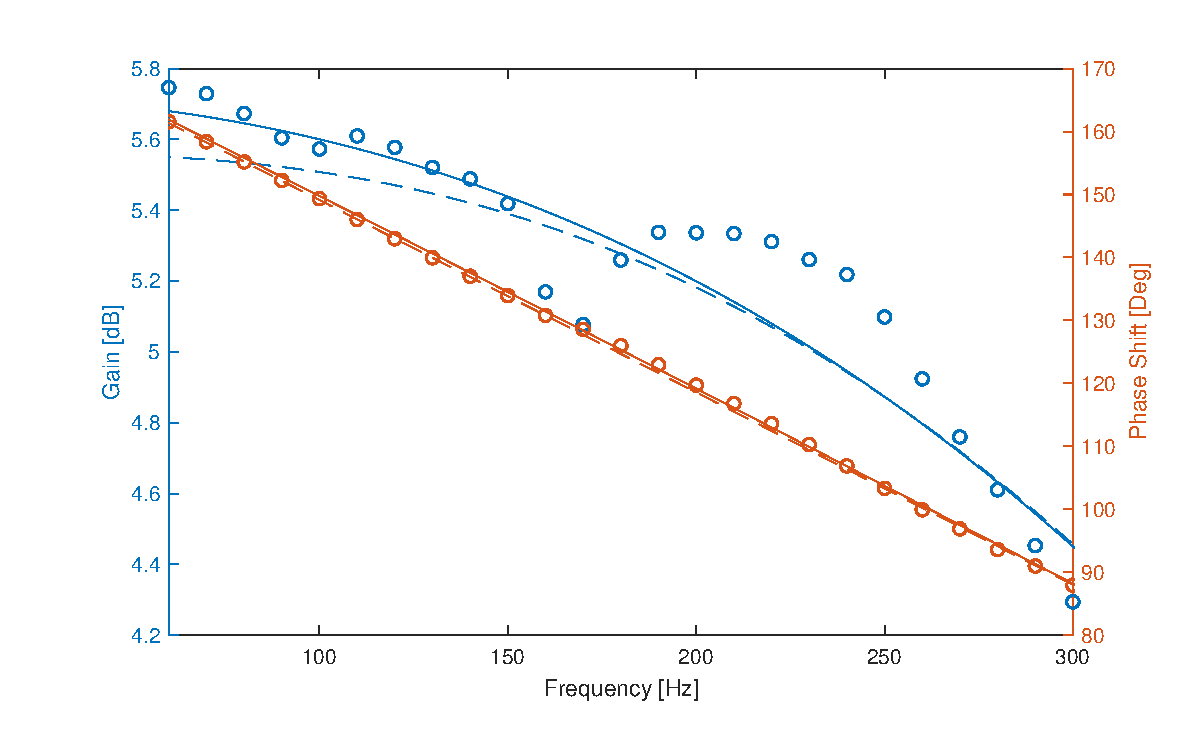
\includegraphics[width=0.95\textwidth]{filter_vs_data.eps}
\subcaption{Beamforming filter}
\label{fig:filter_vs_data}
\end{subfigure}\\
\hspace{0.1\textheight}
\begin{subfigure}[c]{0.5\textwidth}
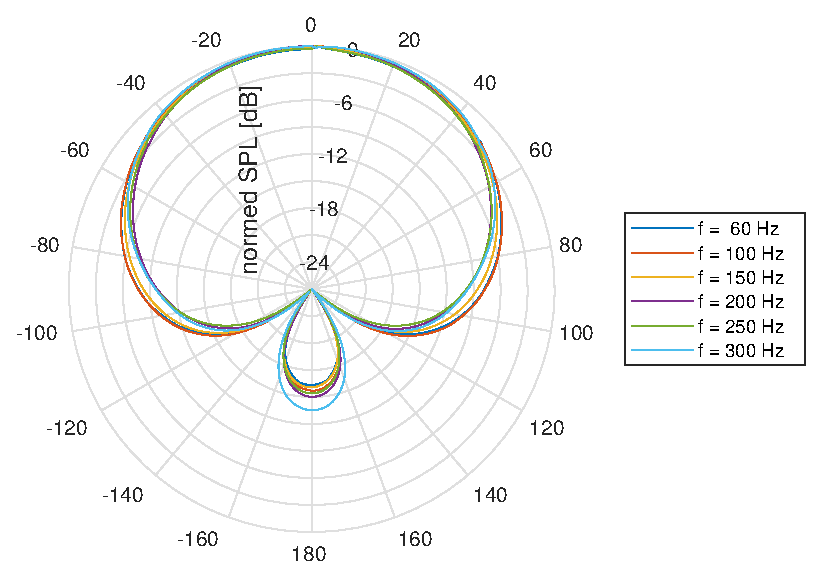
\includegraphics[width=0.95\textwidth]{opt_c.eps}
\subcaption{Directional characteristic, optimal}
\label{fig:opt_res_c}
\end{subfigure}
\begin{subfigure}[c]{0.5\textwidth}
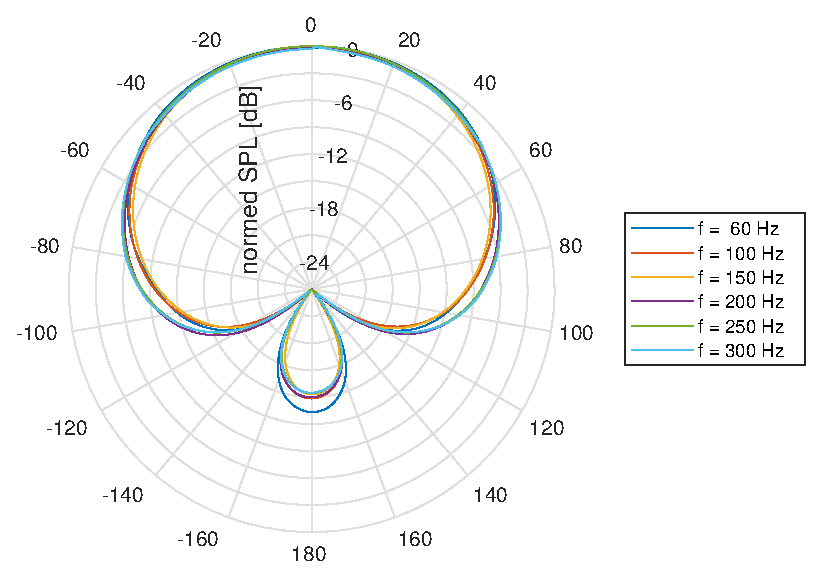
\includegraphics[width=0.95\textwidth]{polar_filtered.eps}
\subcaption{Directional characteristic, filtered}
\label{fig:polar_filtered}
\end{subfigure}
\caption{Filter results, with pressure corrected cost filter, correction table based on Appendix \ref{ax:directional_2}, \textcolor{green3}{\texttt{Lx}}\,$=$\,\SI{0.4}{\meter}, \textcolor{green3}{\texttt{Ly}}\,$=\,$\SI{-0.4}{\meter}}
		\label{fig:opt_res}
\end{figure}


\section{Conclusion}
	\chapter{Numerical Simulation}\label{ch:numerical} 
	\section{The \gls{fdtd}}
The aim of this section is to give the basic of numerical simulation by using \gls{fdtd} method, such that a speaker array sound propagation can be analysed. The method of using numerical simulate will be descried, such that the method can be adapted to one or more speaker in a sound pressure field. 
The theory behind \gls{fdtd} is to solve the wave equation by a finite-difference approximation for both time and space derivatives. This make it possible to easily simulate the sound pressure and particle velocity of a speaker at any time step. One advantage of using \gls{fdtd} is that the impulse response of a specified loudspeaker can be applied to the simulation, and therefore it is possible to simulate the speaker that is used in this project. For using \gls{fdtd} with a specified speaker, all simulation have to be done in a narrow frequency band, before the simulation give a good approximation, the \gls{fdtd} can not include the hole frequency band in one simulation. A second advantage of using \gls{fdtd} is that the calculation is preformed in time domain, which benefit from that the pressure and the particle velocity at a specified time step can be analyzed directly by solving two coupled equation.\citep{fdtddaga}. This section will end out with a \gls{fdtd} model of a 3 dimensional space, where the speaker box does not scatter the simulation \\

\subsection{\gls{fdtd} wave equation}
In \gls{fdtd} simulation, the two equation which need to be solved is the coupled first order equation of the pressure $p$ and the particle velocity $\vec{v}$. The first formula is the Euler \autoref{fdtd_euler}, which describe the relation between the gradient for the pressure $p$ and the derivative of the particle velocity $\vec{v}$ with respect to time \autoref{fdtd_euler}. 

\begin{equation}\label{fdtd_euler}
\frac{\partial \vec{v}}{\partial t} =- \frac{1}{\rho}\vec{\triangledown }p
\end{equation}

    \startexplain
    		\explain{$\rho$ is the density of the medium }{\si{\kilo\gram\per\cubic\meter}}
        \explain{$\partial t$ is an infinitesimal time step}{\si{\second}}
        \explain{$p$ is the pressure }{\si{\pascal}}
        \explain{$\vec{v}$ is the particle velocity}{\si{\meter\per\second}}
    \stopexplain

The \autoref{fdtd_euler} is only valid with small variation of pressure. The second \autoref{fdtd_linear} is the linear continuity equation. The equation describe the relation between derivative of pressure $p$ with respect of time and the velocity $\vec{v}$ gradient. They are combined by the density of the medium and the speed of sound. 

 \begin{equation}\label{fdtd_linear}
\frac{\partial p}{\partial t} =- \rho c^2 \vec{\triangledown }\vec{v}
\end{equation}

    \startexplain
    		\explain{$\rho$ is the density of the medium }{\si{\kilo\gram\per\cubic\meter}}
        \explain{$\partial t$ is an infinitesimal time step}{\si{\second}}
        \explain{$p$ is the pressure }{\si{\pascal}}
        \explain{$c$ is the speed of sound }{\si{\meter\per\second}}
        \explain{$\vec{v}$ is the particle velocity}{\si{\meter\per\second}}
    \stopexplain

Both equation are approximated by using finite difference for every point in space and time, by using a 3 dimensional grid of the space. 


\subsection{\gls{fdtd} using Cartesian grid}

The Cartesian grid for \gls{fdtd} approximation is a well known technique, and will be used in this project \citep{finiteproblems}. The Cartesian grid is using the pressure \autoref{fdtd_linear} and the particle velocity \autoref{fdtd_linear} as the unknown quantities, which have to be solved for every point in space.  A small grid is visualized in \autoref{fig:fdtd_cartesian_grid}

\begin{figure}[H]
	\centering
\begin{picture}(0,0)%
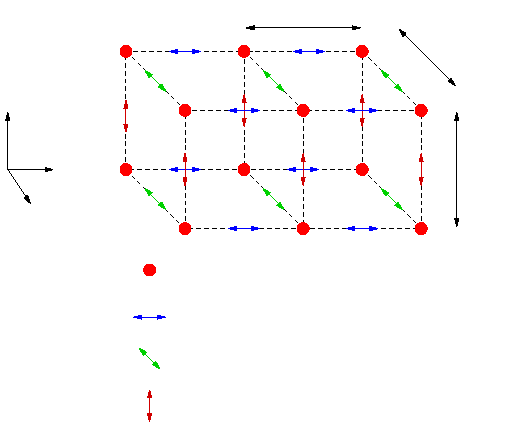
\includegraphics{fdtd_grid.pdf}%
\end{picture}%
\setlength{\unitlength}{4144sp}%
%
\begingroup\makeatletter\ifx\SetFigFont\undefined%
\gdef\SetFigFont#1#2#3#4#5{%
  \reset@font\fontsize{#1}{#2pt}%
  \fontfamily{#3}\fontseries{#4}\fontshape{#5}%
  \selectfont}%
\fi\endgroup%
\begin{picture}(3869,3327)(3541,-1288)
\put(6841,1649){$\delta y$}%
\put(3556,1244){$z$}%
\put(4006,704){$x$}%
\put(3826,344){$y$}%
\put(5806,1874){$\delta x$}%
\put(4996,-61){Pressure point}%
\put(4996,-421){Particle velocity x-direction}%
\put(4996,-781){Particle velocity y-direction}%
\put(4996,-1096){Particle velocity z-direction}%
\put(7066,704){$\delta z$}%
\end{picture}%
	\caption{A 3 dimensional example of Cartesian grid}
		\label{fig:fdtd_cartesian_grid}
\end{figure}


The grid points is build up on positions there is descried as $(i\,\delta x,j\,\delta y,k\,\delta z)$ at time $t=[l]\delta t$, where the time step is visualized in \autoref{fig:fdtd_transient_point}

\begin{figure}[H]
	\centering
\begin{picture}(0,0)%
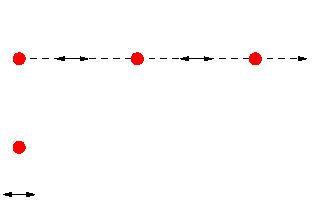
\includegraphics{fdtd_transient_point.pdf}%
\end{picture}%
\setlength{\unitlength}{4144sp}%
%
\begingroup\makeatletter\ifx\SetFigFont\undefined%
\gdef\SetFigFont#1#2#3#4#5{%
  \reset@font\fontsize{#1}{#2pt}%
  \fontfamily{#3}\fontseries{#4}\fontshape{#5}%
  \selectfont}%
\fi\endgroup%
\begin{picture}(2518,1594)(4804,-854)
\put(5266,-421){Pressure point}%
\put(5266,-781){Particle velocity}%
\put(5076,469){$[l-\frac{1}{2}] \delta t$}%
\put(5671, 29){$[l] \delta t$}%
\put(6456, 29){$[l+1]\delta t$}%
\put(5961,469){$[l+\frac{1}{2}]\delta t$}%
\put(7246,254){$t$}%
\end{picture}%
	\caption{Transient definition points of sound $p$ pressure and particle velocity $\vec{v}$}
		\label{fig:fdtd_transient_point}
\end{figure}

$\delta x,\delta y,\delta z$ is the spatial discretization step as shown in \autoref{fig:fdtd_cartesian_grid} and $\delta t$ is the time spatial discretization step as shown in \autoref{fig:fdtd_transient_point}. $i,j,k$ is the discrete indices for the point in grid and $l$ is the discrete time index. For every axis, the component of the particle velocity have to be determined at position in \autoref{fdtd_component} at intermediant time $t=[l\pm\frac{1}{2}]$ 

\begin{equation}\label{fdtd_component}
\vec{v}= \begin{bmatrix}
v_x[(i\pm \frac{1}{2})\,\delta x,j\,\delta y,k\,\delta z]\\
v_y[i\,\delta x,(j\pm \frac{1}{2})\,\delta y,k\,\delta z]\\
v_z[i\,\delta x,j\,\delta y,(k\pm \frac{1}{2})\,\delta z]
\end{bmatrix}
\end{equation}
and the pressure is determined at position $p_{(i,j,k)}^{[l+1]}$. The scaler $\delta t$ is the actual time step, but since the MATLAB and python works with scaler step, $\delta t$ is implemented in the formulas and not in the iteration step. The time $\pm \frac{1}{2}$ is also changed to a scalar with adding $\frac{1}{2}$, but this scalar is only used in the implementation and is leaved out in the rest of this section. The same apply for the step size $\delta x$, $\delta y$ and $\delta z$.\\

The used speaker in this project is a speaker used for air operation, the medium for $\rho$ in the calculation will be air. The following step is done to get the linearized equation for particle velocity in Cartesian grid to any time. First \autoref{fdtd_euler} has to be rewritten to \autoref{fdtd_euler_rewrite_system}.


\begin{subequations}\label{fdtd_euler_rewrite}
\begin{alignat}{2}
-\rho_0 \frac{\partial \vec{v}}{\partial t} &=\vec{\triangledown }p \label{fdtd_euler_rewrite_1}\\
-\rho_0 \frac{\partial \vec{v}}{\partial t} &=\frac{\partial p}{\partial x}\vec{x}+\frac{\partial p}{\partial y}\vec{y}+\frac{\partial p}{\partial z}\vec{z} \label{fdtd_euler_rewrite_2}
\end{alignat}
\end{subequations}

Since $\vec{v}$ is an equation system of three inputs, the \autoref{fdtd_euler_rewrite} is split into an equation system \citep{Sakuma2014}.

\begin{subequations}\label{fdtd_euler_rewrite_system}
\begin{alignat}{2}
\frac{\partial p}{\partial x} &=-\rho_0 \frac{\partial v_x}{\partial t} \label{fdtd_euler_rewrite_system_1}\\
\frac{\partial p}{\partial y} &=-\rho_0 \frac{\partial v_y}{\partial t} \label{fdtd_euler_rewrite_system_2}\\
\frac{\partial p}{\partial z} &=-\rho_0 \frac{\partial v_z}{\partial t} \label{fdtd_euler_rewrite_system_3}
\end{alignat}
\end{subequations}


Next the $v_x$, $v_y$ and $v_z$ have to be differentiated with respect to $t$ and $p$ with respect to $x$, $y$ and $z$. To make it simple when differentiate with $t$ \autoref{fdtd_euler_diff_1} for all $v_x$, $v_y$ and $v_z$ only the $v_x$ is showed. The differentiation with $v_y$ and $v_z$ is trivial but only the indices is at there respectively indices. When differentiate with respect to $x$, $y$ and $z$ in \autoref{fdtd_linear_diff_2} only the differentiate with respect to $x$ is done. The differentiation with respect to $y$ and $z$ is also trivial and only the indices is at there respectively indices \citep{Sakuma2014}.



\begin{subequations}\label{fdtd_euler_diff}
\begin{alignat}{2}
\frac{\partial v_x}{\partial t}\mid _{(i+\frac{1}{2},j,k)}^{[l]} &= \frac{(v_x)_{(i+\frac{1}{2},j,k)}^{[l+\frac{1}{2}]} -(v_x)_{(i+\frac{1}{2},j,k)}^{[l-\frac{1}{2}]}}{\delta t} \label{fdtd_euler_diff_1} \\
\frac{\partial p}{\partial x}\mid _{(i+\frac{1}{2},j,k)}^{[l]} &= \frac{p_{(i+1,j,k)}^{[l]} -p_{(i,j,k)}^{[l]}}{\delta x}  \label{fdtd_linear_diff_2}
\end{alignat}
\end{subequations}

Substituting \autoref{fdtd_euler_diff} intro \autoref{fdtd_euler_rewrite_system} and solve for $(v_x)_{(i+\frac{1}{2},j,k)}^{[l+\frac{1}{2}]}$ leads to following three \autoref{fdtd_particle_velocity}


\begin{subequations}\label{fdtd_particle_velocity}
\begin{alignat}{2}
(v_x)_{(i+\frac{1}{2},j,k)}^{[l+\frac{1}{2}]}&= (v_x)_{(i+\frac{1}{2},j,k)}^{[l-\frac{1}{2}]}-\frac{\delta t}{\rho_0 \delta x} \left( p_{(i+1,j,k)}^{[l]} -p_{(i,j,k)}^{[l]}  \right)\\
(v_y)_{(i,j+\frac{1}{2},k)}^{[l+\frac{1}{2}]}&= (v_y)_{(i,j+\frac{1}{2},k)}^{[l-\frac{1}{2}]}-\frac{\delta t}{\rho_0 \delta y} \left( p_{(i,j+1,k)}^{[l]} -p_{(i,j,k)}^{[l]}  \right)\\
(v_z)_{(i,j,k+\frac{1}{2})}^{[l+\frac{1}{2}]}&= (v_z)_{(i,j,k+\frac{1}{2})}^{[l-\frac{1}{2}]}-\frac{\delta t}{\rho_0 \delta z} \left( p_{(i,j,k+1)}^{[l]} -p_{(i,j,k)}^{[l]}  \right)
\end{alignat}
\end{subequations}
\\

The following step is done to get the linearized equation for pressure in Cartesian grid to any time. First \autoref{fdtd_linear} has to be rewritten to \autoref{fdtd_linear_rewrite_2}

\begin{subequations}\label{fdtd_linear_rewrite}
\begin{alignat}{2}
- \frac{1}{\rho_0c^2} \frac{\partial p}{\partial t} &=\vec{\triangledown }\vec{v} \label{fdtd_linear_rewrite_1}\\
- \frac{1}{\rho_0c^2} \frac{\partial p}{\partial t} &=\frac{\partial v_x}{\partial x}+\frac{\partial v_y}{\partial y}+\frac{\partial v_z}{\partial z}\label{fdtd_linear_rewrite_2}
\end{alignat}
\end{subequations}
\\


Next the $p$ have to be differentiated with respect to $t$ and $v_x$, $v_y$ and $v_z$ with respect to $x$, $y$ and $z$ respectively as done in \autoref{fdtd_linear_diff}. As in \autoref{fdtd_euler_diff} only the differentiation to $t$ and $x$ is done \citep{Sakuma2014}.



\begin{subequations}\label{fdtd_linear_diff}
\begin{alignat}{2}
\frac{\partial p}{\partial t}\mid _{(i,j,k)}^{[l+\frac{1}{2}]} &= \frac{p_{(i,j,k)}^{[l+1]} -p_{(i,j,k)}^{[l]}}{\delta t} \label{fdtd_linear_diff_1}\\
\frac{\partial v_x}{\partial x}\mid _{(i,j,k)}^{[l+\frac{1}{2}]} &= \frac{(v_x)_{(i+\frac{1}{2},j,k)}^{[l+\frac{1}{2}]} -(v_x)_{(i-\frac{1}{2},j,k)}^{[l+\frac{1}{2}]}}{\delta x} \label{fdtd_euler_diff_2}
\end{alignat}
\end{subequations}


Substituting \autoref{fdtd_linear_diff} intro \autoref{fdtd_linear_rewrite_2} and solve for $p_{(i,j,k)}^{[l+1]}$ leads to  \autoref{fdtd_pressure}




\begin{multline}\label{fdtd_pressure}
p_{(i,j,k)}^{[l+1]} = p_{(i,j,k)}^{[l]} - \rho_0 c^2 \delta t \Biggl( \frac{(v_x)_{(i+\frac{1}{2},j,k)}^{[l+\frac{1}{2}]} - (v_x)_{(i-\frac{1}{2},j,k)}^{[l+\frac{1}{2}]}}{\delta x} \\ 
+ \frac{(v_y)_{(i,j+\frac{1}{2},k)}^{[l+\frac{1}{2}]}-(v_y)_{(i,j-\frac{1}{2},k)}^{[l+\frac{1}{2}]}}{\delta y} +  \frac{(v_z)_{(i,j,k+\frac{1}{2})}^{[l+\frac{1}{2}]}-(v_z)_{(i,j,k-\frac{1}{2})}^{[l+\frac{1}{2}]}}{\delta z} \Biggr)
\end{multline}

\subsection{\gls{fdtd} grid boundary conditions}        
The meaning of the boundary condition is the condition near and at the wall. The sound wave react different on the walls than when it is propagating in free field. Wall will act like a reflecting surface, absorbing surface or both. This boundary behaviour from the wall is descried as an impedance which is frequency dependent. This have to be analysed and implemented in the simulation because the sound field will be different compare to sound field without any boundary. The frequency dependency boundary will only be a good approximation and not accurate in this project. An accurate frequency dependency model will require heavy calculation with convolution at each boundary point at each time step \citep{finiteproblems}. This kind of calculation have a high time consumption and therefore an approximation will be used. \\
The approximation in this project will then be based on the above description which use the impedance approach \citep{FDTDmodelling}. The impedance approach can be used when wall is present in simulation, and can not make a perfect matched layer. Therefore the impedance approach can not be used in free field simulation unless the simulation is stopped just before the wave hits the boundary. The simulation stopping will give some area in every corner where the wave do not have reach and will give a hard stopping circular shape. In this project a large room is used and the simulation will be stopped just before the boundary to simulate free field condition. Afterwards the data is cropped such that only simulating data within the circular shape is used. \\

The  impedance approach is usable at low frequency \citep{FDTDmodelling}, two kind of absorbing boundary are common in real life and therefore also in simulation. this boundary is as following:

\begin{enumerate}
\item Thin absorbing boundary with respect to wavelength on a much harder background e.g wall and roof absorbers and seats.
\item Light nonstiff walls e.g. plaster walls and curtain 
\end{enumerate}


The behaviour of the first material (1) can roughly be approximated to be a complex frequency dependent impedance \autoref{fdtd_thin_absorbing}

\begin{equation}\label{fdtd_thin_absorbing}
Z= Z_0+\frac{Z_{-1}}{j\omega}
\end{equation}

         \startexplain
    		\explain{$Z$ is the }{\si{1}}
        \explain{$Z_0$ is the}{\si{1}}
        \explain{$Z_{-1}$ is the }{\si{1}}
         \explain{$j$ is the complex $j$ in this context }{\si{1}}
         \explain{$\omega$ is the angle speed }{\si{1}}
    \stopexplain

The behaviour of the second material (2) can quite accurate be approximated to be a complex frequency dependent impedance \autoref{fdtd_light_absorbing}

\begin{equation}\label{fdtd_light_absorbing}
Z= Z_0+j\omega M
\end{equation}

         \startexplain
    		\explain{$Z$ is the }{\si{1}}
         \explain{$M$ is the mass per unit square meter of the boundary}{\si{1}}
    \stopexplain

 \citep{finiteproblems} propose a general approximated impedance \autoref{fdtd_general_absorbing} of \autoref{fdtd_thin_absorbing} and \autoref{fdtd_light_absorbing}, which is useful for \gls{fdtd} simulation in low frequency.

\begin{equation}\label{fdtd_general_absorbing}
Z(\omega)= Z_0+\frac{Z_{-1}}{j\omega}+j\omega Z_1
\end{equation}

         \startexplain
    		\explain{$Z_1$ is the }{\si{1}}
    		\explain{$Z(\omega)$ is an expansion of the frequency impedance impedance around the frequency of interest }{\si{1}}
    \stopexplain
    
In time domain \autoref{fdtd_general_absorbing} can be expressed as the boundary condition \autoref{fdtd_boundary_absorbing}

\begin{equation}\label{fdtd_boundary_absorbing}
p(t)= Z_0v_n(t)+Z_1\int_{-\infty}^{t} v_n(\tau)d\tau +Z_1\frac{\partial u_n(t)}{\partial t} 
\end{equation}

         \startexplain
    		\explain{$p(t)$ is the acoustics pressure}{\si{\pascal}}
    		\explain{$v_n(t)$ is the component of the particle velocity orthogonal to the boundary plan}{\si{\meter\per\second}}
    \stopexplain

One arising problem in this method is that the particle velocity at the boundary, when the boundary is at plan $x=(i_0+0.5)\delta x$, which is the boundary at the $x$ velocity plan, cannot be calculated by using the pressure at $p_{(i_0+1,j,z)}$ and the same is applicable for $y$ and $z$ plan. The problem is visualized in \autoref{fig:fdtd_boundary_pressure} in 1 dimension.

\begin{figure}[H]
	\centering
\begin{picture}(0,0)%
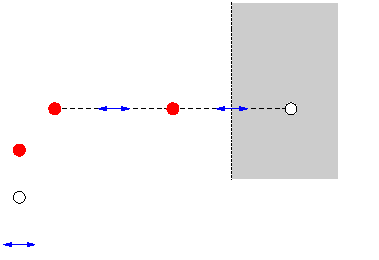
\includegraphics{fdtd_wall_reflection.pdf}%
\end{picture}%
\setlength{\unitlength}{4144sp}%
%
\begingroup\makeatletter\ifx\SetFigFont\undefined%
\gdef\SetFigFont#1#2#3#4#5{%
  \reset@font\fontsize{#1}{#2pt}%
  \fontfamily{#3}\fontseries{#4}\fontshape{#5}%
  \selectfont}%
\fi\endgroup%
\begin{picture}(2876,1975)(4534,-854)
\put(4996,-61){Pressure point}%
\put(4996,-781){Particle velocity x-direction}%
\put(4996,-421){Unknown pressure point}%
\end{picture}%
	\caption{The figure visualized a boundary plan through particle velocity plan $x$ in 1 dimension.}
		\label{fig:fdtd_boundary_pressure}
\end{figure}

For solving the problem visualized in \autoref{fig:fdtd_boundary_pressure}, an asymmetric finite-difference approximation for the space derivative is used  \citep{finiteproblems}. \autoref{fdtd_boundary_absorbing} shows the asymmetric finite-difference approximation.

\begin{equation}\label{fdtd_boundary_absorbing_velocity}
\frac{\partial p}{\partial x}\mid _{(i_0+\frac{1}{2},j,k)}^{[l]} = \frac{2}{\delta x} \left( p_{(i_0+\frac{1}{2},j,k)}^{[l]}-p_{(i_0,j,k)}^{[l]} \right)
\end{equation}\\

The advance of \autoref{fdtd_boundary_absorbing_velocity} is that it only require knowledge of one nearest pressure point, but it is only valid within $\delta x$. \autoref{fdtd_boundary_absorbing} can then be used to express  \autoref{fdtd_boundary_absorbing} as function of $v_x$. Using the same procedure as in \autoref{fdtd_particle_velocity} just with plugging in \autoref{fdtd_boundary_absorbing_velocity} instead, the particle velocity at the boundary is approximated as \autoref{fdtd_boundary_eqp}

\begin{equation}\label{fdtd_boundary_eqp}
(v_x)_{(i_0+\frac{1}{2},j,k)}^{[l+\frac{1}{2}]}= (v_x)_{(i_0+\frac{1}{2},j,k)}^{[l-\frac{1}{2}]}-\frac{2 \delta t}{\rho_0 \delta x} \Biggl( 
p_{(i_0+\frac{1}{2},j,k)}^{[l]} -p_{(i_0,j,k)}^{[l]}  \Biggr)
\end{equation}

The only unknown in \autoref{fdtd_boundary_eqp} is $p_{(i_0+\frac{1}{2},j,k)}^{[l]}$ but can be founded by using \autoref{fdtd_boundary_absorbing}, where $v_n$ is changed with $(v_x)_{(i_0+\frac{1}{2},j,k)}^{[l]}$ and become \autoref{fdtd_boundary_velocity}


\begin{multline}\label{fdtd_boundary_velocity}
(v_x)_{(i_0+\frac{1}{2},j,k)}^{[l+\frac{1}{2}]}= (v_x)_{(i_0+\frac{1}{2},j,k)}^{[l-\frac{1}{2}]}-\frac{2 \delta t}{\rho_0 \delta x} \Biggl( 
 Z_0(v_x)_{(i_0+\frac{1}{2},j,k)}^{[l]} \\
 +Z_1 \frac{\partial (v_x)_{(i_0+\frac{1}{2},j,k)}^{[l]}}{\partial t} +Z_{-1} \int_{-\infty}^{t} (v_x)_{(i_0+\frac{1}{2},j,k)}^{[l]}(\tau)d\tau -p_{(i_0,j,k)}^{[l]}
\Biggr)
\end{multline}

The integral in the \autoref{fdtd_boundary_velocity2} is replaced with a sum from minus infinity to $l$ in \autoref{fdtd_boundary_absorbing}.

\begin{multline}\label{fdtd_boundary_velocity2}
(v_x)_{(i_0+\frac{1}{2},j,k)}^{[l+\frac{1}{2}]}= (v_x)_{(i_0+\frac{1}{2},j,k)}^{[l-\frac{1}{2}]}-\frac{2 \delta t}{\rho_0 \delta x} \Biggl( 
 Z_0(v_x)_{(i_0+\frac{1}{2},j,k)}^{[l]} \\
+Z_1\frac{(v_x)_{(i+\frac{1}{2},j,k)}^{[l+\frac{1}{2}]}-(v_x)_{(i+\frac{1}{2},j,k)}^{[l-\frac{1}{2}]}}{\delta t}+Z_{-1} \delta t \sum_{m=-\infty}^{l} \left( (v_x)_{(i+\frac{1}{2},j,k)}^{[m+\frac{1}{2}]} \right) -p_{(i,j,k)}^{[l]}
\Biggr)
\end{multline}

The last unknown variable is the particle velocity $v_x$ at time $t=[l]$. To find a solution for $v_x$ at time  $t=[l]$  a linear interpolation between $v_x$ at time $t=[l \pm \frac{1}{2}]$ is used \citep{finiteproblems}. The resulting particle velocity will be expressed as \autoref{fdtd_boundary_result}

\begin{multline}\label{fdtd_boundary_result}
(v_x)_{(i_0+\frac{1}{2},j,k)}^{[l+\frac{1}{2}]}= \alpha (v_x)_{(i_0+\frac{1}{2},j,k)}^{[l-\frac{1}{2}]} + \beta \frac{2 \delta t}{\rho_0 \delta x} \Biggl( 
 Z_0(v_x)_{(i_0+\frac{1}{2},j,k)}^{[l]} \\
-Z_{-1} \delta t \sum_{m=-\infty}^{l} \left( (v_x)_{(i+\frac{1}{2},j,k)}^{[m+\frac{1}{2}]} \right) -p_{(i,j,k)}^{[l]}
\Biggr)
\end{multline}


         \startexplain
    		\explain{$\alpha = \frac{1-\frac{Z_0}{Z_{FDTD}} \frac{2Z_1}{Z_{FDTD}} \delta t}{1+\frac{Z_0}{Z_{FDTD}} \frac{2Z_1}{Z_{FDTD}} \delta t}$ }{\si{1}}
    		\explain{$\beta = \frac{1}{1-\frac{Z_0}{Z_{FDTD}} \frac{2Z_1}{Z_{FDTD}} \delta t}$ }{\si{1}}
    		\explain{$Z_{FDTD} = \frac{\rho_0 \delta x}{\delta t}$ }{\si{1}}
    \stopexplain



\subsection{\gls{fdtd} grid cell size}

The chose of grid cell size for \gls{fdtd} is a critical variable which must hold some specified constrain \citep{Kunz1993}. The grid cell size have to be small enough to contain data for all specified simulated frequency, which mean that the grid cell size have to be smaller than the smallest wavelength $\lambda$. When the frequency rise the wave length is decreasing. This mean the grid cell size constrain is determined by the highest frequency of interest in the \gls{fdtd} simulation. The grid cell size also have to be as a certain size such that the computation resource is kept down. The grid cell size therefore have to be chosen intelligent which \citep{Kunz1993} display one solution. After the grid cell size is chosen the Courant stability condition determined the maximum time step. The maximum time step size which will be calculated based on the grid cell size will be the used time step size because smaller time step size do not improve the accuracy generally. \\


The boundary for the lowest grid cell size is the Nyquist rate, which state that the wavelength shall at least be twice as big as the grid cell size $\delta$. Since $\delta x$, $\delta y$ and $\delta z$ have the same size only $\delta$ will be used for grid step size. The Nyquist rate is the lower boundary, but since the simulation is an approximation an is not exact and the smallest wavelength is not precise, $\delta$ have to be more than two samples per wavelength. To find a optimal grid size the grid dispersion error which relate to the wave speed through the grid will be taken intro account. The error occurs because the wave propagate slightly with different speed through the grid and this error also depending on the relative direction of the wave. The grid dispersion error is propertional to the grid cell size, which mean that the error minimized with smaller $\delta$\citep{Kunz1993}. 

Often if $ \delta \leq \frac{1}{10}\lambda_{min}$ the above constrain is met, and is therefore a good compromise between computation resource and approximation error. The grid cell size in this project is therefore as in \autoref{fdtd_delta_stepsize}

\begin{equation}\label{fdtd_delta_stepsize}
\delta x = \delta y = \delta z \leq \frac{1}{10} \frac{c}{f_{max}}
\end{equation}

    \startexplain
    		\explain{$\delta$ is the grid cell size }{\si{1}}
        \explain{$x$, $y$ and $z$ is the direction}{\si{1}}
        \explain{$c$ is the speed of sound}{\si{\meter\per\second}}
        \explain{$f_{max}$ is the maximum frequency in the simulation}{\si{\hertz}}
    \stopexplain
    
    
    

\subsection{\gls{fdtd} time step size and stability}   \label{sec:fdtd_time_stepsize} 
The time step size for \gls{fdtd} follows from the Courant condition \citep{Kunz1993}. The aim of the project is not to analyse the condition of Courant, this section will then explain shortly about the importers of the condition and use the condition to calculate the time step size. Consituring a plane wave, the Courant condition state that in one time step any point on the wave must not pass through more than one cell, during one time step the wave can propagate only from one cell to its nearest neighbors \citep{Kunz1993}. To determine the time step size the time step $\delta t $ can therefore be determined by the speed of light and the grid cell size as in \autoref{fdtd_time_stepsize}



\begin{equation}\label{fdtd_time_stepsize}
\delta t \leq \frac{1}{\sqrt{\frac{1}{(\delta x)^2}+\frac{1}{(\delta x)^2}+\frac{1}{(\delta x)^2} }\cdot c}
\end{equation}
        \startexplain
    		\explain{$\delta$ is the time size}{\si{1}}
        \explain{$t$ is the time indicator}{\si{1}}
        \explain{$c$ is the speed of sound}{\si{\meter\per\second}}
    \stopexplain
    
Making the step size smaller than \autoref{fdtd_time_stepsize} will not improve the result, in fact the equation calculate the time step size where the grid dispersion error is minimized \citep{Kunz1993}. Unless the dispersion error is minimized, the time step might even be  smaller because of stability condition. 
A stable simulation is only guaranteed under surtain condition. Because \autoref{fdtd_boundary_result} is applied to different condition e.g. in corner or flat walls, a stable simulation is not possible in general, only with surtain condition which depend on time and grid cell size. It have be shown that the simulation is stable if $Z_0$ and $Z_{1}$ is all positive and for all simulation regions if \autoref{fdtd_time_stepsize_boundary} is satisfied \citep{finiteproblems}.

\begin{equation}\label{fdtd_time_stepsize_boundary}
\delta t \leq \sqrt{\frac{2}{3}}  \left( \frac{1}{\sqrt{\frac{1}{(\delta x)^2}+\frac{1}{(\delta x)^2}+\frac{1}{(\delta x)^2} }\cdot c} \right)
\end{equation}\\


If $Z_{-1}$ is nonzero the time step shall furthermore satisfy \autoref{fdtd_time_stepsize_boundary_Z_n1}

\begin{equation}\label{fdtd_time_stepsize_boundary_Z_n1}
c \delta t \leq \delta x \left(   \frac{1+\frac{2Z_1}{\rho_0 \delta x}}{1+\frac{2Z_{-1} \delta x}{\rho_0 c^2}}  \right)^{\frac{1}{2}}
\end{equation}

\subsection{\gls{fdtd} sound source}
It have to be remembered that the acoustical center of the speaker is about \SI{17}{\centi\meter} in the front of the speaker \autoref{sec:ac_center}. It also have to be noted that the \gls{fdtd} sound source is at the acoustical center and not at the speaker position, and therefore the \gls{fdtd} sound source is a transparent source. The speaker box may do a different in real measurement but not at the \gls{fdtd} sound source position and therefore the speaker box will not be included in the \gls{fdtd} sound source model. The following section will shortly explain the three most common source \citep{FDTDsource},  and explain the use of a transparent source. \\

There is two easy ways to implement a \gls{fdtd} sound source and one more advanced way to implement a \gls{fdtd} sound source. The easy way to implementing at sound source is the hard- and the soft source. The problem with implementing a hard source is that the hard source overwrite the update step in the source point and therefore effectively scatter any incident field. This might be a real scenario if the speaker box was at the acoustical center, but it is not and therefore this kind of source is not present for this simulation. Second the soft source benefit from that the pressure from the source is added to the pressure source point, and this source do not scatter. The problem with this method is that the actual excitation does not match the time function of the source. To make a source that act like a hard source but do not scatter, the transparent source is used according to \citep{FDTDtransparent}. The transparent source will shortly be explained in this section. \\



A transparent source is reached by measuring the impulse response $I$ of the grid and use it in \autoref{fdtd_transparent_source}

\begin{multline}\label{fdtd_transparent_source}
p_{(i_{s},j_{s},k_{s})}^{[l+1]}=p_{(i_{s},j_{s},k_{s})}^{[l]} - \rho_0 c^2 \delta t  \Biggl( \frac{(v_x)_{(i_{s}+\frac{1}{2},j_{s},k_{s})}^{[l+\frac{1}{2}]} - (v_x)_{(i_{s}-\frac{1}{2},j_{s},k_{s})}^{[l+\frac{1}{2}]}}{\delta x} +
 \frac{(v_y)_{(i_{s},j_{s}+\frac{1}{2},k_{s})}^{[l+\frac{1}{2}]}-(v_y)_{(i_{s},j_{s}-\frac{1}{2},k_{s})}^{[l+\frac{1}{2}]}}{\delta y} + \\ 
 \frac{(v_z)_{(i_{s},j_{s},k_{s}+\frac{1}{2})}^{[l+\frac{1}{2}]}-(v_z)_{(i_{s},j_{s},k_{s}-\frac{1}{2})}^{[l+\frac{1}{2}]}}{\delta z} \Biggr)
+f^{l+1}-\sum_{m=0}^{l} \left( I^{l-m+1}f^m \right)
\end{multline}

        \startexplain
        \explain{$(i_{s},j_{s},k_{s})$ is the source grid position}{\si{1}}
        \explain{$I$ is the impulse response of the grid}{\si{1}}
    \stopexplain

As it can be seen in \autoref{fdtd_transparent_source}, the source is implemented like a soft source but with a correction part $-\sum_{m=0}^{l} \left( I^{l-m+1}f^m \right)$. The correction part include the impulse response of the \gls{fdtd} grid and have to be measured. To measure the impulse response of the grid, a Kronecker delta function is used as the sound source with unity gain. The Kronecker delta source give an impulse with unity gain only at time one, and zero otherwise. The Kronecker delta source is implemented as a hard source \citep{FDTDtransparent}. \\


The impulse response is measured at the source point, but it have to be noted that the impulse response is not the Kronecker delta function unless it is measured in the same point. The impulse response is the value the source pressure point should have been calculated to according to the particle velocity. But since the Kronecker delta is implemented as a hard source, the source pressure point will be overwritten by the Kronecker delta function and therefore the impulse response step have to be calculated from the nearest particle velocity. The impulse response measurement function is therefore \autoref{fdtd_transparent_source_impulse}

\begin{multline}\label{fdtd_transparent_source_impulse}
I^{[l]}=p_{(i_{s},j_{s},k_{s})}^{[l-1]} - \rho_0 c^2 \delta t  \Biggl( \frac{(v_x)_{(i_{s}+\frac{1}{2},j_{s},k_{s})}^{[l-\frac{1}{2}]} - (v_x)_{(i_{s}-\frac{1}{2},j_{s},k_{s})}^{[l-\frac{1}{2}]}}{\delta x} +\\
 \frac{(v_y)_{(i_{s},j_{s}+\frac{1}{2},k_{s})}^{[l-\frac{1}{2}]}-(v_y)_{(i_{s},j_{s}-\frac{1}{2},k_{s})}^{[l-\frac{1}{2}]}}{\delta y} +  
 \frac{(v_z)_{(i_{s},j_{s},k_{s}+\frac{1}{2})}^{[l-\frac{1}{2}]}-(v_z)_{(i_{s},j_{s},k_{s}-\frac{1}{2})}^{[l-\frac{1}{2}]}}{\delta z} \Biggr)
\end{multline}


The Kronecker delta source will be placed in the middle of the grid, and there is only one Kronecker delta source. The particle velocity matrices for each dimension have therefore the following symmetrical $(v_x)_{(i_{s}-\frac{1}{2},j_{s},k_{s})}^{[l-\frac{1}{2}]} = -(v_x)_{(i_{s}+\frac{1}{2},j_{s},k_{s})}^{[l-\frac{1}{2}]}$. The impulse response measurement function can therefore be shorted to \autoref{fdtd_transparent_source_impulse_short}

\begin{equation}\label{fdtd_transparent_source_impulse_short}
I^{[l]}=p_{(i_{s},j_{s},k_{s})}^{[l-1]} - 2\rho_0 c^2 \delta t  \Biggl( \frac{(v_x)_{(i_{s}+\frac{1}{2},j_{s},k_{s})}^{[l-\frac{1}{2}]}}{\delta x} +
 \frac{(v_y)_{(i_{s},j_{s}+\frac{1}{2},k_{s})}^{[l-\frac{1}{2}]}}{\delta y} +  
 \frac{(v_z)_{(i_{s},j_{s},k_{s}+\frac{1}{2})}^{[l-\frac{1}{2}]}}{\delta z} \Biggr)
\end{equation}

There is a stability condition there have to be satisfied before the transparent source is stable in \gls{fdtd} simulation. The stability condition is \autoref{fdtd_transparent_source_impulse_stability} \citep{FDTDtransparent}. 


\begin{equation}\label{fdtd_transparent_source_impulse_stability}
\frac{c \delta t}{\delta x} \leq \frac{1}{\sqrt{N}}
\end{equation}

        \startexplain
        \explain{$N$ is the number of dimension}{\si{1}}
    \stopexplain
    
    
\subsection{\gls{fdtd} conclusion}
It can be concluded that is it possible to simulate one or more source in a \gls{fdtd} simulation. It is possible to make simulation in room and in free field condition. The free field simulation require that the simulation is stopped just before the sound wave hits the wall, and only the data inside the wave circular shape is used. It can also be concluded that that the sound source have to be transparent in all \gls{fdtd} simulation, because the scatter from a hard source do not represent real world scenario. In real world measurement, the speaker box will inflict the measurement by scattering, but the scattering will be much different and depend on the speaker box position. The acoustical center can be in the same point with different position of the speaker box, and therefore if the speaker box should have been in the simulation, the speaker box should have been placed at the exact point. The scattering also change compare to the shape of the speaker box, and therefore a \gls{fdtd} model of the box is required. In this simulation the speaker box \gls{fdtd} model is not investigated and will be leaved out of the simulation 


  
		\section{\gls{fdtd} simulation} \label{sec:fdtd_simulation}
The aim of this chapter is to make a simulation of the zero order gradient speaker, first order gradient speaker and the solution proposed in \autoref{sec:opt_result} using \gls{fdtd}. All simulation cross all three different method of using speaker at low frequency will be compared in both free field and inside a room. The result will be discussed with respect to directionality and efficiency. 

\section{\gls{fdtd} simulations step size}
This section will determined the the step size for both grid size and the time step size. As the time step size is depending on the grid step size, the grid step size will be determined first. Recalling \autoref{fdtd_delta_stepsize} state that all three dimention will have the same step size in this project, the calculation is as following \autoref{fdtd_distance_stepsize} 

\begin{subequations}\label{fdtd_distance_stepsize}
\begin{alignat}{2}
d &= \delta x = \delta y = \delta z= \frac{1}{10} \frac{c}{f_{max}} \label{fdtd_distance_stepsize_1}\\
d &= \frac{1}{10} \frac{\SI{343}{\meter\per\second}}{\SI{300}{\hertz}} \label{fdtd_distance_stepsize_2}\\
d &= \SI{0.11}{\meter} \label{fdtd_distance_stepsize_3}
\end{alignat}
\end{subequations}

    \startexplain
    		\explain{$d$ is the grid cell size }{\si{\meter}}
        \explain{$c$ is the speed of sound at 20 degree}{\si{\meter\per\second}}
        \explain{$f_{max}$ is the maximum frequency in the simulation}{\si{\hertz}}
    \stopexplain
    
The time step have to be small enough such that standard walls can be included in the simulation, and since plaster wall is well used, $Z_{1}$ is possible nonzero and therefore both condition in \autoref{sec:fdtd_time_stepsize} has to be satisfied. The first condition is \autoref{fdtd_time_stepsize_boundary} stated as following \autoref{fdtd_time_stepsize_con_one}
    
 
    \begin{subequations}\label{fdtd_time_stepsize_con_one}
\begin{alignat}{2}
\delta t &\leq \sqrt{\frac{2}{3}}  \left( \frac{1}{\sqrt{\frac{1}{(\delta x)^2}+\frac{1}{(\delta x)^2}+\frac{1}{(\delta x)^2} }\cdot c} \right)\\
\delta t &\leq \sqrt{\frac{2}{3}}  \left( \frac{1}{\sqrt{\frac{1}{(\SI{0.11}{\meter})^2}+\frac{1}{(\SI{0.11}{\meter})^2}+\frac{1}{(\SI{0.11}{\meter})^2} }\cdot \SI{343}{\meter\per\second}} \right)\\
\delta t &\leq \SI{0.157}{\milli\second} 
\end{alignat}
\end{subequations}
    
 Which correspond to a sampling frequency of at least \SI{6364}{\hertz}. The second condition is \autoref{fdtd_time_stepsize_boundary_Z_n1} where plaster is chosen as the limit case for soft walls and concrete is chosen as the limit for hard walls. The calculation for plaster walls is as following \autoref{fdtd_time_stepsize_con_plaster} \citep{finiteproblems}.
 
     \begin{subequations}\label{fdtd_time_stepsize_con_plaster}
\begin{alignat}{2}
c \delta t &\leq \delta x \left(   \frac{1+\frac{2Z_1}{\rho_0 \delta x}}{1+\frac{2Z_{-1} \delta x}{\rho_0 c^2}}  \right)^{\frac{1}{2}}\\
 \delta t &\leq \frac{\SI{0.11}{\meter} \left(   \frac{1+\frac{2\cdot 6}{1.21 \cdot \SI{0.11}{\meter}}}{1+\frac{2 \cdot 16 \cdot \SI{0.11}{\meter}}{1.21 \cdot {343}^2}}  \right)^{\frac{1}{2}}}{343}\\
\delta t &\leq \SI{3.12}{\milli\second} 
\end{alignat}
\end{subequations}
 Which correspond to a sampling frequency of at least \SI{320}{\hertz}.


concrete is missing??


It can be concluded that the grid step size $d$ shall be \SI{114}{\milli\meter} and the sampling frequency $\frac{1}{\delta t}$ shall at least be equal or higher than \SI{6364}{\hertz}, The impulse response from the used \gls{dut} will be used as the impulse response in all simulation. All impulse response measurement in this project have a sample frequency of \SI{44.1}{\kilo\hertz} but because the simulation does not have to have higher sample frequency than \SI{6364}{\hertz}, the sample frequency of the measurement will be down sampled with a factor of 6. The choose of a factor of 6 is justified by that this is the highest scalar factor the measurement sampling frequency can be down sampled  and still satisfy the minimum sampling frequency and also keeping the required process power down. This result in a sampling frequency for the simulation of \SI{7.35}{\kilo\hertz}

\section{\gls{fdtd} algorithm}
The aim of this section is to convert the grid to matrices. Since the grid is in three dimension, the whole matrix system for pressure will build on a three dimensional matrix and all particle velocity matrices will built on three dimensional matrices. The following \autoref{} shows an extended grid with entry notation of \autoref{fig:fdtd_cartesian_grid}








 

%%

\part{Test and Discussion}\label{pt:test}
\graphicspath{{figures/tests/}}
	\chapter{Performance Evaluation}
		%In this section, all tests will be made and the fulfillments will be marked in a table in the end of each test section, where the following marks will indicate if the test is approved, conditionally approved or not fulfilled.
 \vspace{1cm}
    \startexplain
     \explain{\cmark  \hspace{4mm} is approved}{$\cdot$}
     \explain{\cmark* \hspace{1mm} is conditionally approved}{$\cdot$}
     \explain{\xmark \hspace{5mm} is not fulfilled}{$\cdot$}
    \stopexplain
	\chapter{Comparison: Simulations and Measurement}
	\chapter{Comparison: Array vs Single Speaker}


 
%%
\part{Conclusion}\label{pt:conclusion}
%\section{Discussion}\label{sec:discussion}

In \autoref{pt:tests} all the requirements were tested to see if they can be approved. It is seen that out the 26 stated requirements, 16 are approved, six are partially approved and four are not approved.
\autoref{req:delay1} is approved, but some additions have to be made to make it function as a usable delay effect. The reason of this is that the time between the echoes is too short. With the implemented buffer size it is only possible to produce a delay time of \SI{41}{\micro\second}, which is too short. 
The six requirements that are partially approved are all related to the missing user interface. The user interface was not implemented due to the time limit of the project and the fact that it was chosen to make the implementation of the effects the main focus. The six partially approved requirements are categorized as such, because it is possible to change the required parameters, but only through changing them directly in the program. 
The first requirement that is not approved is \autoref{req:SNR}. It was measured that the \gls{dsp} has a \gls{snr} of \SI{39.91}{\decibel}, which is lower than the \gls{snr} in the guitar. The low \gls{snr} in the \gls{dsp} means that it will not even be enough to re-design the effects to make them as noiseless as possible.  
The second requirement that is not approved is \autoref{req:power2}, where the reason is that the \gls{dsp} is powered by a \SI{5}{\volt} USB supply. Since the supply voltage that is now used is smaller than the stated \SI{9}{\volt}, this requirement can be approved if a \SI{9}{\volt} supply is used to make a \SI{5}{\volt} supply for the \gls{dsp}.
The third and fourth requirement that are not approved are \autoref{req:flanger1} and \autoref{req:chorus1}. The reason of this is that the implemented \gls{cordic} algorithm is not able to produce sine waves with lower frequencies than \SI{0.4}{\hertz}, because with 32-bit precision sine and cosine values for frequencies less than \SI{0.4}{\hertz} can not be represented. A solution to this would therefore be to use a higher bit precision. \\
%The fifth requirement that is not approved is \autoref{req:preamp3}, because the measured output impedance of the preamp is measured to \SI{9.06}{\kilo\ohm}, which should be smaller than \SI{2}{\kilo\ohm}. The result of the measurement is questionable because the output impedance of an \gls{opamp} normally lies around \SI{50}{\ohm} to \SI{200}{\ohm}. \\

Some choices than were made in the development of the project can be discussed. One of them is the decision of implementing all the effects entirely in assembly. The reason behind the decision was to make the effects run as fast as possible, to get familiar with the assembly language, and to get a better understanding of the \gls{dsp}. It is seen in \autoref{app:effect_run_time}, that each effect uses approximately one tenth of the sampling period to complete its program. This indicates that it might have been possible to implement parts of effects in the slower, but faster implementable language C. This approach might have left time for implementing the user interface for instance. 
Another discussion is whether the resolution of the calculations in the effects should be increased from 16- to 32-bits. This will improve the sound quality of the effects. It was seen in the development of the \gls{cordic} calculations that increasing the precision, made it possible to to produce sine waves of lower frequencies. The resolution could of course always be a parameter that could be improved, but the noticeable difference from going from 16- to 32-bits, might be larger going from 32- to 64-bits. It has to be taken into account that higher resolution would require more memory.  
A subject for discussion is the approach for developing the effects, the \gls{reverb} for example. In this specific case, a Moorer \gls{reverb} unit was chosen. The reason of this decision was to have some guidelines for developing a \gls{reverb} effect. When looking back, it might have been beneficial to design the effect without relying as much on a reference. This might have improved the possibility  of making the effect sound as intended. \\

For further enhancements, several steps could be made towards improving the product. One of them is the user interface, which would not only make it possible to approve more of the requirements, but also make the final product more usable. One would for example not have stop and reprogram the \gls{dsp} to change effect, or even to just change one parameter in an effect. 
Additional developments can also be finishing the implementation of the designed effects but also the missing parts in the already implemented ones in assembly, such as implementing the attenuating part of the equalizer or making the \gls{cordic} algorithm able to produce different oscillations at the same time to finish the chorus effect. 
Moreover, a parameter that can be investigated more is the noise in the system. It could be investigated if it in some way is possible to improve the \gls{snr} in the \gls{dsp}. 
%

\glsresetall
\appendix % Start of appendix
\addtocontents{toc}{\protect\setcounter{tocdepth}{0}} 
%\input{chapters/appendices/_appendices} % Include appendices
%Appendix:

 \graphicspath{{figures/appendix/}}
\part{Appendix}\label{pt:appendix}
\section{Outline ...}
In this appendix the control of the Outline turntable will be descriped    
\chapter{Measurement of Directional Characteristics I}\label{ax:directional_1}
This appendix serves as a protocol to a series of measurements conducted on the 23\textsuperscript{rd} of February 2018 in the large anechoic chamber (B4-111) at the acoustical lab of Aalborg University at Fredrik Bajers Vej 7.\\
The goal of these measurements was to try out and evaluate a MATLAB-based measurement routine to quantify the directional characteristic of loudspeakers, especially gaining experience with determining the acoustical center of a loudspeaker.

\section*{Measuring Equipment and Materials}
The following measuring equipment was used:
\begin{itemize}[noitemsep]
\item Microphone \gls{bandk} 4144
\begin{itemize}[noitemsep]
\item AAU-number: 06552
\item Serial number: 297090
\end{itemize}
\item Preamplifier GRAS 26AK
\begin{itemize}[noitemsep]
\item AAU-number: 56525
\item Serial number: 32811
\end{itemize}
\item Power supply \gls{bandk} 2804
\begin{itemize}
\item AAU-number: 06998
\item Serial number: 455309
\end{itemize}
\item Calibrator \gls{bandk} 4231
\begin{itemize}[noitemsep]
\item AAU-number: 33691
\item Serial number: 2115338
\end{itemize}
\item Power Amplifier Pioneer A-616
\begin{itemize}[noitemsep]
\item AAU-number: 08249
\item Serial number: HJ9404841S
\end{itemize}
\item Sound card RME Fireface UCX
\begin{itemize}[noitemsep]
\item AAU-number: 108230
\item Serial number: 23811948
\end{itemize}
\item Turntable: Outline ET 250-3D
\begin{itemize}
\item Serial number: REIBO012
\end{itemize}
\item MATLAB r2017b on OSX 10.11.6
\item Loudspeaker SEAS 33 F-WKA
\end{itemize}

The following material was used:
\begin{itemize}[noitemsep]
%\item \SI{1/2}{\inch} to \SI{1}{\inch} preamp adapter
\item Microphone clip
\item Microphone stand
\item LEMU cable
\item XLR cable
\item Ethernet cable
\item Loudspeaker stand
\item Loudspeaker cabinet, plywood, outside dimensions: (400x400x400)\SI{}{\milli\meter}, wall thickness: \SI{20}{\milli\meter}
\end{itemize}

\section*{Setup}
A sketch of the measurement setup can be found in \autoref{fig:measurement_setup}. A picture is given in \autoref{fig:setup_02_23}

\begin{figure}[htbp]
	\centering
	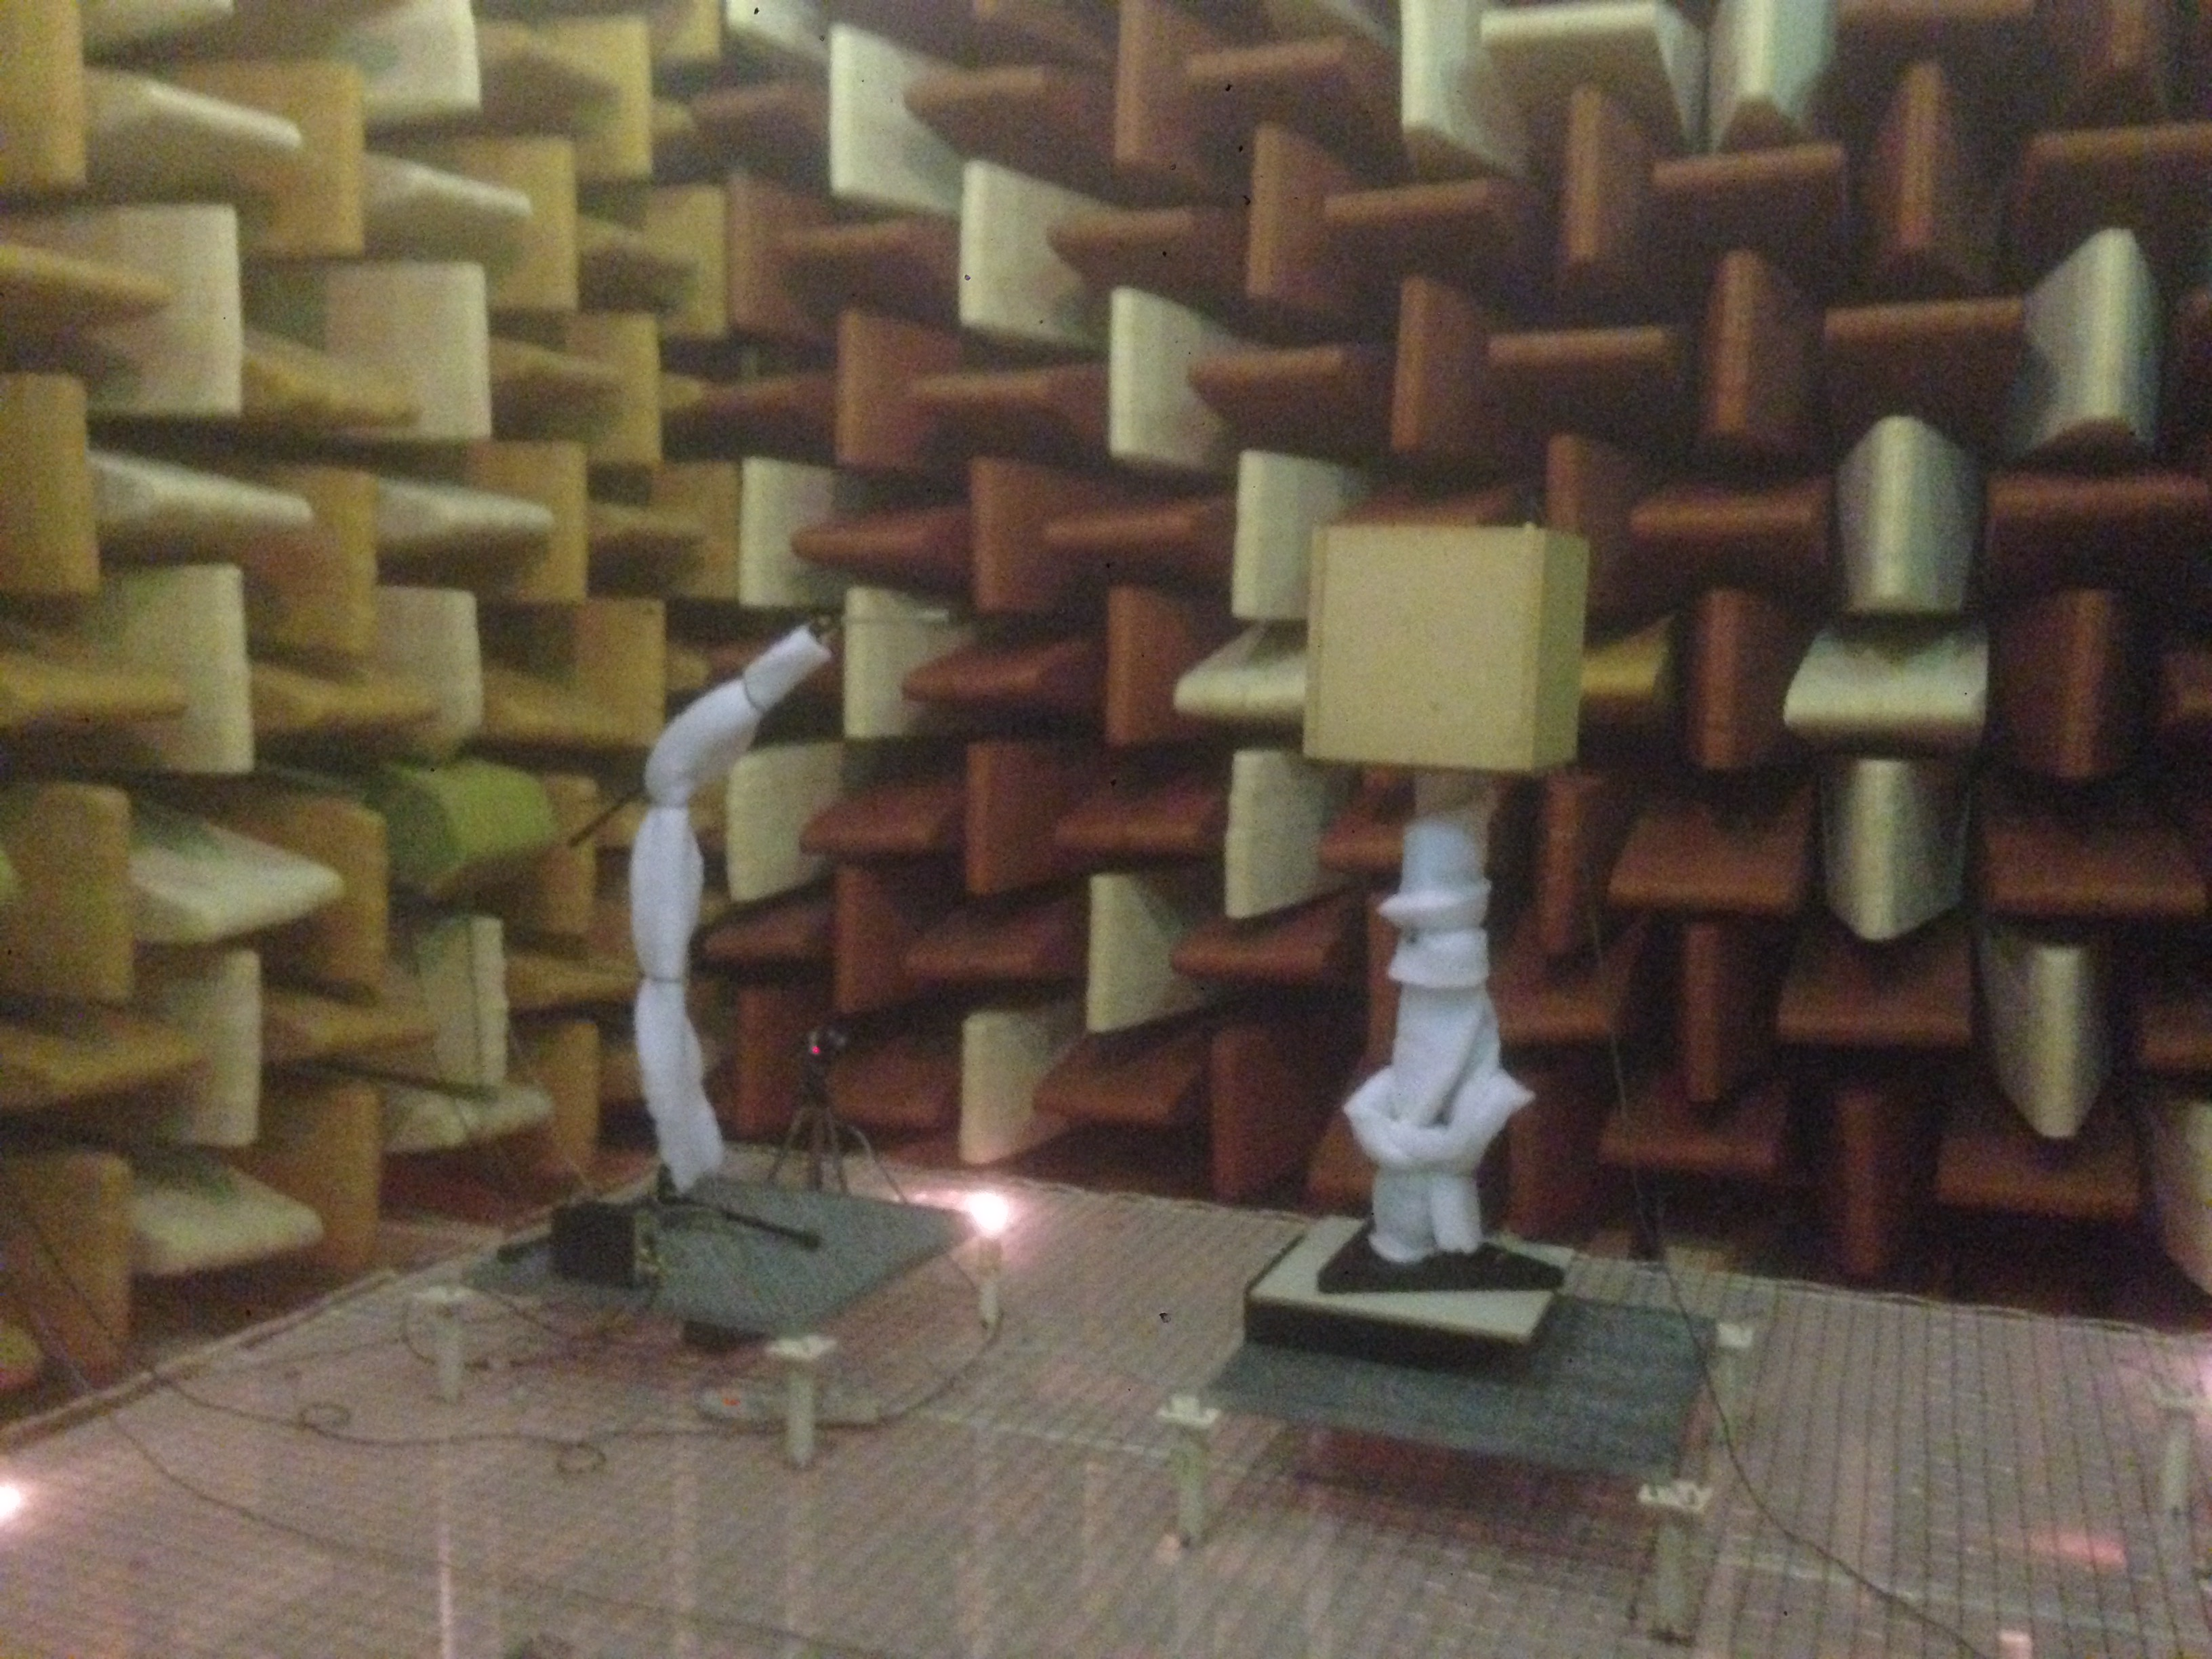
\includegraphics[width=0.7\textwidth]{02_23_setup.JPG}
	\caption{Measurement setup}
		\label{fig:setup_02_23}
\end{figure}

The horizontal distance between the microphone and the edge of the cabinet was \SI{0.75}{\meter}. This rather short distance was deliberately chosen for the sake of testing the measurement setup and getting an idea of the position of the acoustic center of the speaker. Directivity measurements should be conducted in the far field. In the frequency range that this project is covering, this means, that loudspeaker and microphone have to be placed significantly further apart. Because of the early stage of development, in which the measurement routine was at the point in time, that the measurement took place, no output calibration was applied. This means, that all measurement results are only relative and have no link to physical units that have been measured.

\section*{Results}
The measurement results have to be viewed remembering, that this measurement series has to be considered a practice run before the actual measurement to characterize the directivity characteristics of the speaker. \autoref{fig:02_23_pressure} shows the results of a measurement conducted at a distance \(d=\) \SI{0.75}{\meter} to the front plane of the speaker. The \gls{spl} normed to the level on the main axis is displayed along the radial coordinate. The angular coordinate describes the position of the microphone in relation to the main axis of the speaker. The coloured lines relate to different frequencies.
The shape of the \SI{60}{\hertz} curve appears to be quite similar to a circle. However, it is not concentric with the pole. Several reasons seem likely to cause this behaviour.  First of all the distance between the microphone and the speaker does not correspond to far field conditions in this frequency range. Secondly, the speaker may not behave as an ideal omnidirectional source and at last the acoustical center of the speaker might have been misplaced off the rotational axis of the turn table.\\
It can be seen, that the pressure on the back side of the speaker keeps decreasing for rising frequencies, especially around approx. \SI{120}{\degree} and \SI{240}{\degree}.

\begin{figure}[htbp]
	\centering
	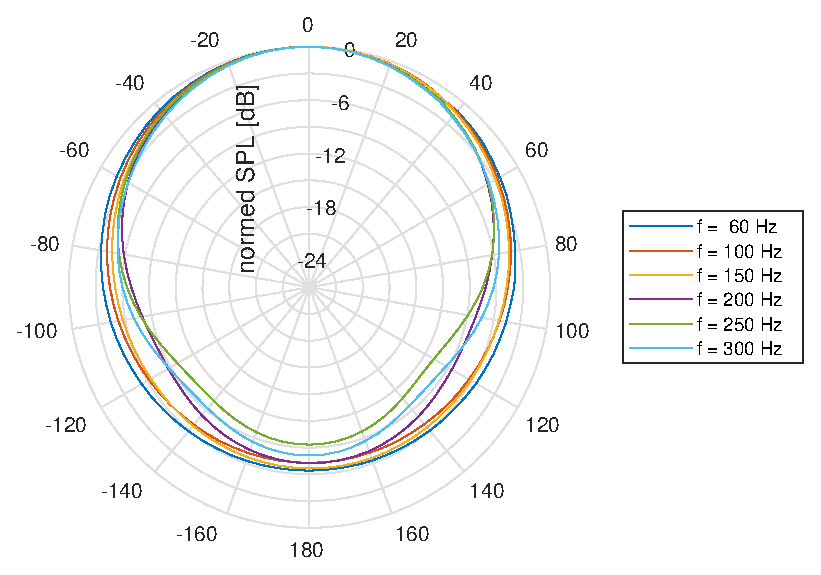
\includegraphics[width=0.7\textwidth]{02_23_pressure.eps}
	\caption{Normed \gls{spl}, measured at a distance \(d=\)\SI{0.75}{\meter}}
		\label{fig:02_23_pressure}
\end{figure}

In order to further investigate the position of the acoustical center in relation to the rotational axis of the turntable, a look at \autoref{fig:02_23_phase} might yield more information. The phase displayed along the radial coordinate. The colours correspond to the same frequencies as in \autoref{fig:02_23_pressure}. It has to be noted, that the phase angle, that is shown in the plot does not necessarily represent the phase angle of the sound pressure related to the motion of the loud speaker membrane, because the phase characteristic of the auto interface and the amplifier were not taken into account via calibration. The phase angles can therefore only be viewed relative to eachother. Similar to the \autoref{fig:02_23_pressure}, the graphs appear to be circular at least at the lower frequencies, but not concentric with the pole.\\
When interpreting these curves, one must take the definition of the acoustical center from \autoref{sec:ac_center} into account. Because the acoustical center is defined the position of a point source, it is to be expected that around a circumference around this point source the signal at any measurement point should be in phase. This would correspond to a concentric circle on the plot. The shifted circles in the polar plot indicate, that the acoustical center has been in front of the rotational axis of the turntable during the measurement. It might be possible to calculate the offset out of the phase data (see \autoref{sec:ac_center}). This however has to be verified in later measurements (see \autoref{ax:directional_2}).\\
The shape of the phase graph tends to look more like a cardiod towards higher frequencies. This might possibly be a general tendency but could also be influenced by the comparatively short distance between the microphone and the speaker. 

\begin{figure}[htbp]
	\centering
	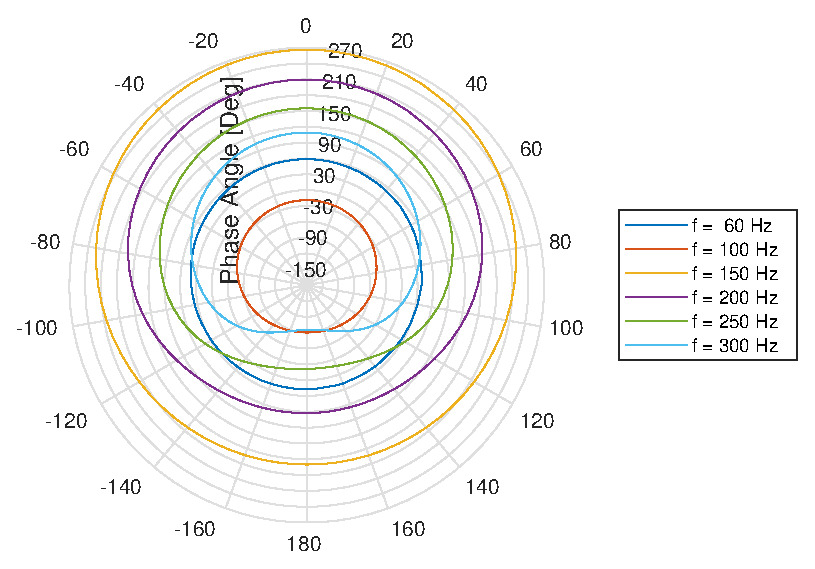
\includegraphics[width=0.7\textwidth]{02_23_phase.eps}
	\caption{Phase (uncalibrated), measured at a distance \(d=\)\SI{0.75}{\meter}}
		\label{fig:02_23_phase}
\end{figure}

\chapter{Measurement of Directional Characteristics II}\label{ax:directional_2}
This appendix serves as a protocol to a series of measurements conducted on the 2\textsuperscript{nd} of March 2018 in the large anechoic chamber (B4-111) at the acoustical lab of Aalborg University at Fredrik Bajers Vej 7.\\
The goal of these measurements was to quantify the directional characteristics of the loudspeakers that will be used in the loudspeaker array. The results are useful to show, what assumptions can be made when the speaker array is set up and where the position of the acoustic center is in relation to the cabinet. They will also serve as a baseline to which the directional characteristics of the speaker array can be compared. Furthermore, more experience can be gained regarding the practical aspects of measurement.

\section*{Measuring Equipment and Materials}
The following measuring equipment was used:
\begin{itemize}[noitemsep]
\item Microphone \gls{bandk} 4144
\begin{itemize}[noitemsep]
\item AAU-number: 06552
\item Serial number: 297090
\end{itemize}
\item Preamplifier GRAS 26AK
\begin{itemize}[noitemsep]
\item AAU-number: 56525
\item Serial number: 32811
\end{itemize}
\item Power supply \gls{bandk} 2804
\begin{itemize}
\item AAU-number: 06998
\item Serial number: 455309
\end{itemize}
\item Calibrator \gls{bandk}\ 4231
\begin{itemize}[noitemsep]
\item AAU-number: 33691
\item Serial number: 2115338
\end{itemize}
\item Power Amplifier Pioneer A-616
\begin{itemize}[noitemsep]
\item AAU-number: 08249
\item Serial number: HJ9404841S
\end{itemize}
\item Sound card RME Fireface UCX
\begin{itemize}[noitemsep]
\item AAU-number: 108230
\item Serial number: 23811948
\end{itemize}
\item Turntable: Outline ET 250-3D
\begin{itemize}
\item Serial number: REIBO012
\end{itemize}
\item MATLAB r2017b on OSX 10.11.6
\item Loudspeaker SEAS 33 F-WKA
\end{itemize}

The following material was used:
\begin{itemize}[noitemsep]
%\item \SI{1/2}{\inch} to \SI{1}{\inch} preamp adapter
\item Microphone clip
\item Microphone stand
\item LEMU cable
\item XLR cable
\item Ethernet cable
\item Loudspeaker stand
\item Loudspeaker cabinet, plywood, outside dimensions: (400x400x400)\SI{}{\milli\meter}, wall~thickness:~\SI{20}{\milli\meter}
\item Speaker mount for turntable
\begin{itemize}[noitemsep]
\item Circular \gls{mdf} cutout, thickness: \SI{12}{\milli\meter}, {\(\varnothing\)~:~\SI{800}{\milli\meter}}
\item Top plate (\gls{mdf}), thickness: \SI{12}{\milli\meter}, surface : (400x400)\SI{}{\milli\meter}
\item 3 battens, (40x40x900)\SI{}{\milli\meter}
\item 3 aluminium brackets
\item 8 bolts M8x30, associated washers
\item miscellaneous woodscrews

\end{itemize}
\end{itemize}

\section*{Setup}
A sketch of the measurement setup can be found in \autoref{fig:measurement_setup}. A picture is given in \autoref{fig:setup_03_02}. \\
According to the findings from \autoref{ax:directional_1} the cabinet had to be backwards from the center of the turntable in order to get the acoustic center of the loudspeaker on the rotational axis. This put up a considerable challenge on the mechanical side.
The 13'' loudspeaker and the cabinet add up to a comparatively large mass. The further they are moved away from the center of the turntable, the more significant are the issues arise, caused by leverage and inertia. This also manifests in \autoref{sec:03_02_results}.
In order to place the the speaker away from the center of the turntable, a circular plane with a diameter of \SI{800}{\milli\meter} was cut out of \SI{12}{\milli\meter} thick \gls{mdf} board and mounted to the turntable. In order to minimize the influence of reflections from the \gls{mdf} board on the measurement, the speaker was raised by \SI{1}{\meter} utilizing wooden pillars. The board on which the loudspeaker rests has the same (400x400)\SI{}{\milli\meter} size as the bottom side of the cabinet. This allows for minor positioning adjustments.\\
Both the microphone and the loudspeaker had a vertical distance of \SI{1.32}{\meter} to the metal grids on which they were standing. The microphone was placed on the main axis of the loudspeaker. The horizontal distance between the front plane of the speaker cabinet and the microphone membrane was \(d=\)\SI{2.74}{\meter}.
The gain potentiometer of the power amplifier was set to \SI{-16}{\decibel} and the \texttt{playgain}-parameter (see XXXXXXX) was set to \SI{-18}{\decibel}.

\begin{figure}[htbp]
	\centering
	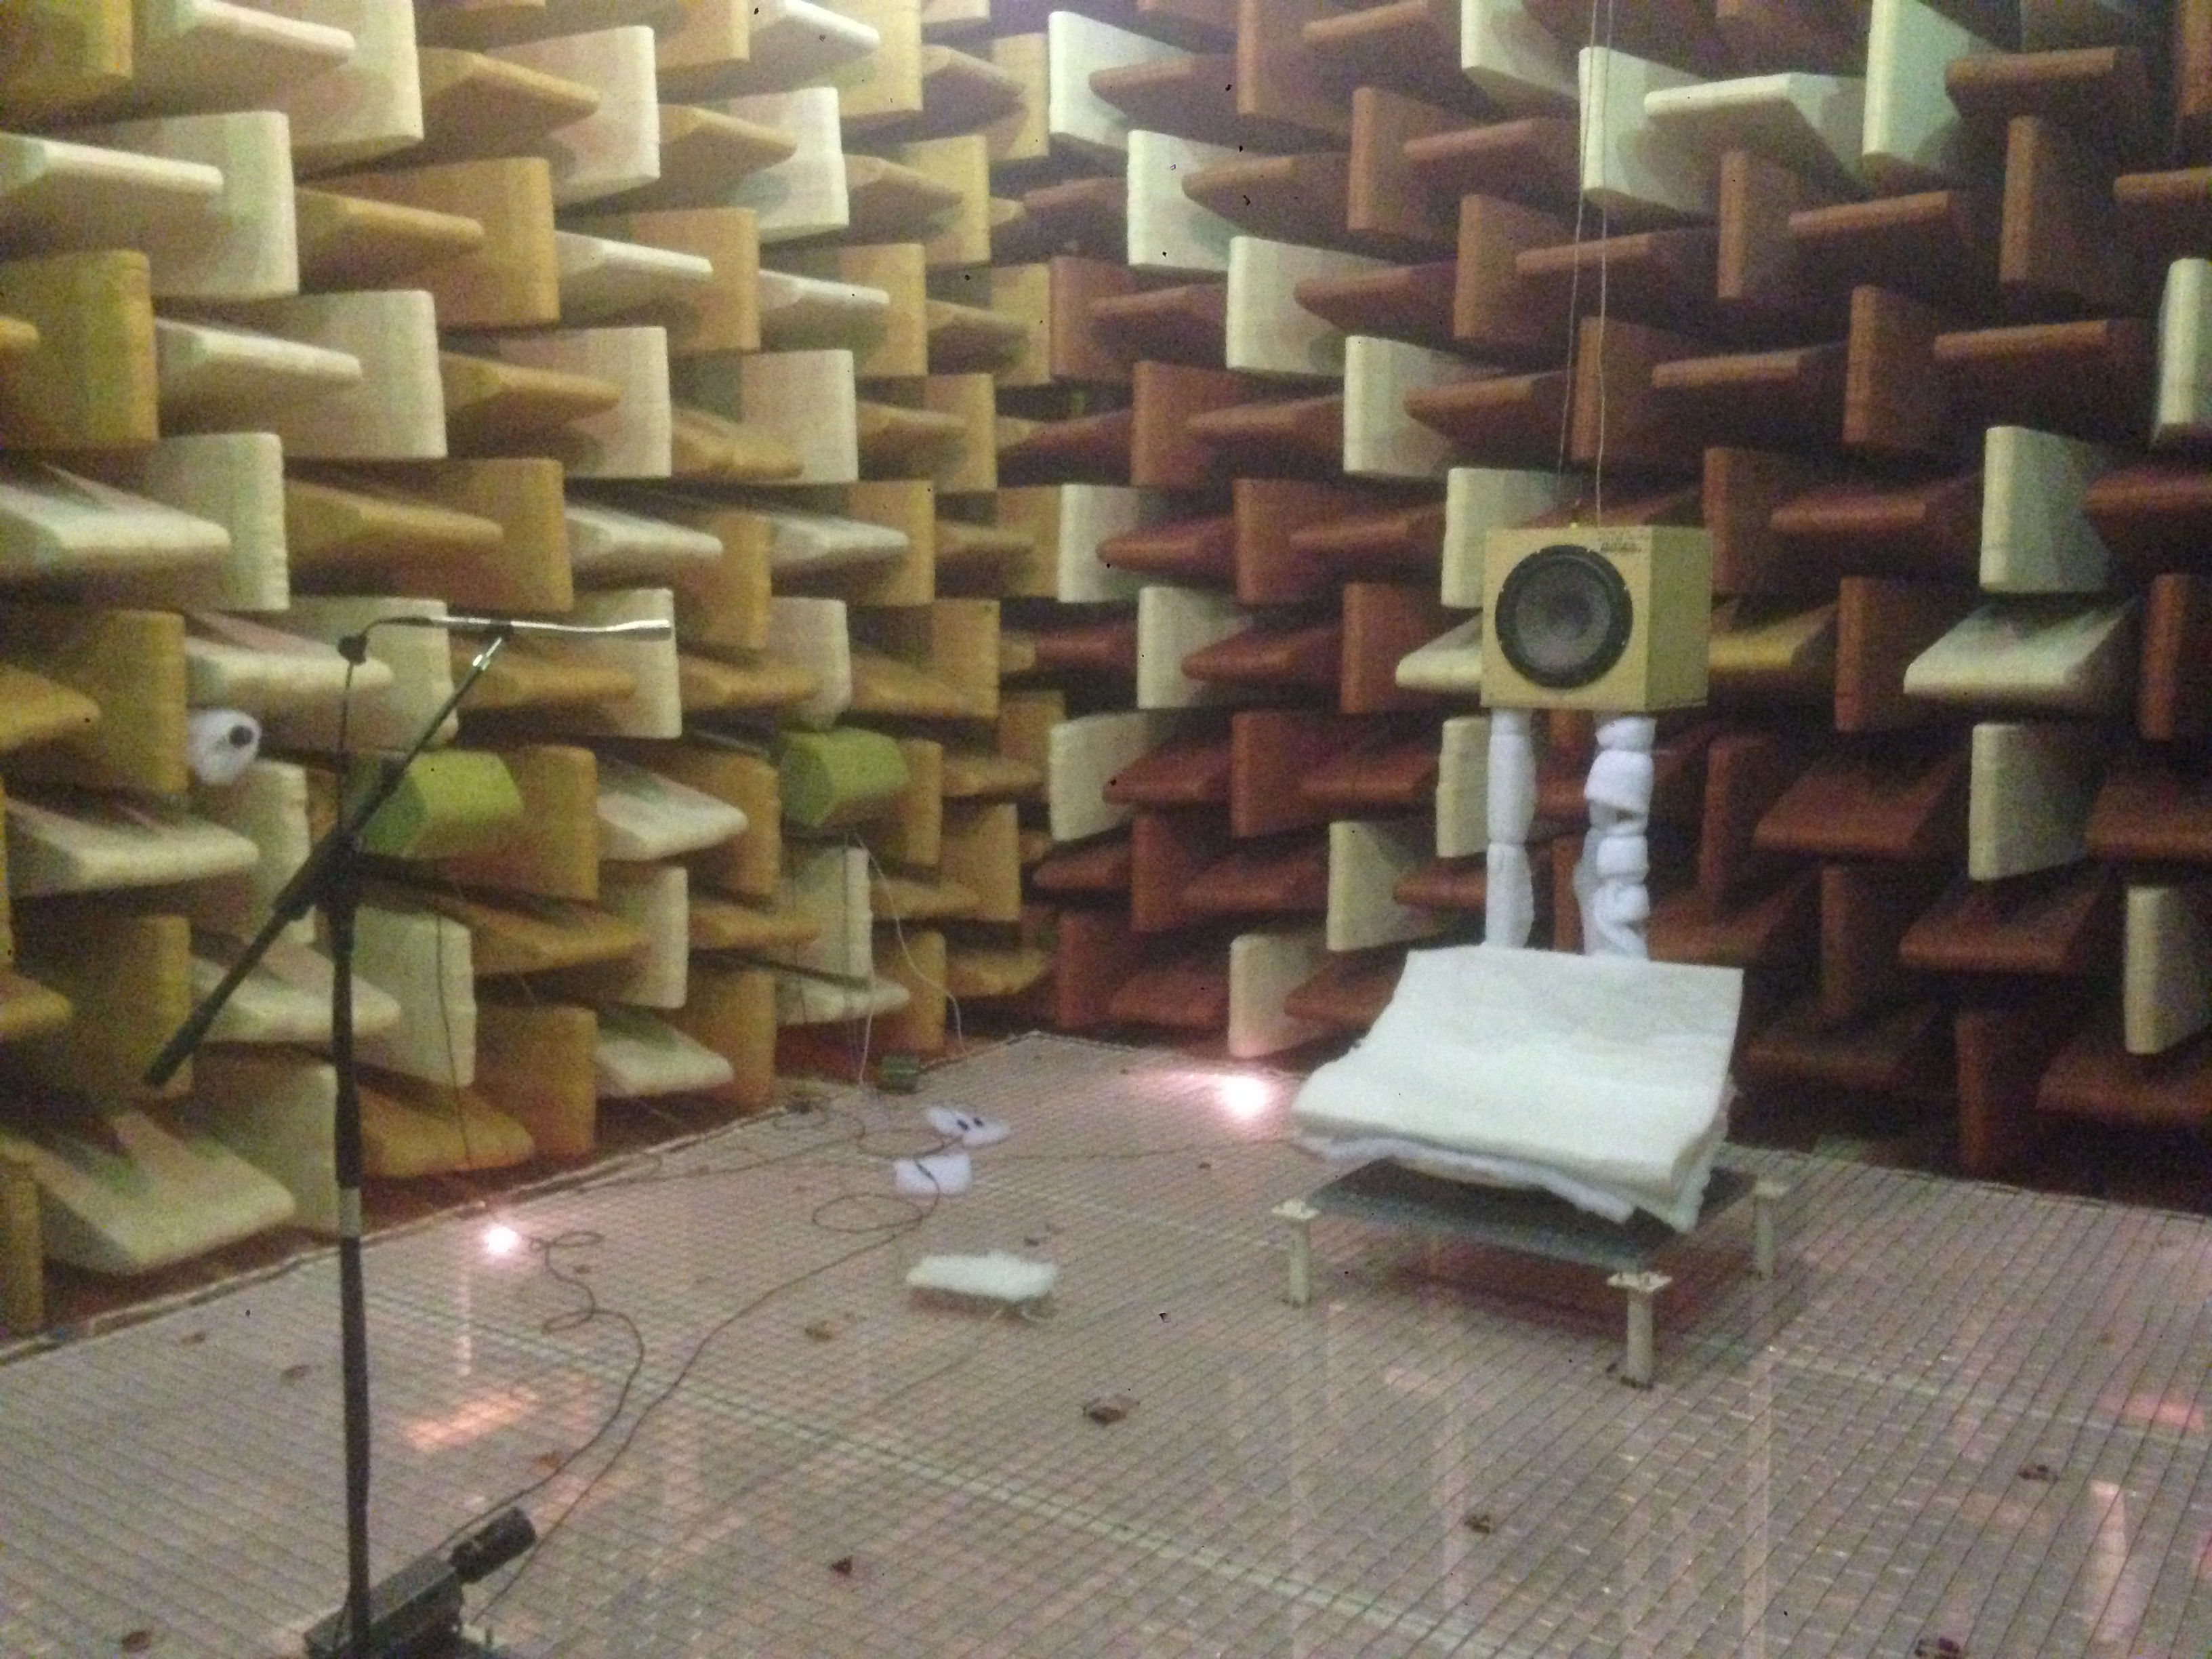
\includegraphics[width=0.7\textwidth]{03_02_setup.JPG}
	\caption{Measurement setup}
		\label{fig:setup_03_02}
\end{figure}

\section*{Results}\label{sec:03_02_results}
The polar response is represented in \autoref{fig:03_02_m1_pressure} and \autoref{fig:03_02_m1_phase}. The front plane of the cabinet had a distance of \SI{115}{\milli\meter} to the rotational axis of the turntable.\\
\autoref{fig:03_02_m1_pressure} shows the normed sound pressure level  along the circumference at different frequencies. The level difference  between the \SI{0}{\degree} and the \SI{180}{\degree} data point is approx. \SI{0.4}{\decibel} at the frequencies of \SI{60}{\hertz} and \SI{100}{\hertz}. Until \SI{150}{\hertz} the graphs have an almost circular shape, that is slightly offset towards the \SI{0}{\degree}. The remaining graphs towards higher frequencies tend to have a shape that is different from that of a circle.
\begin{figure}[htbp]
	\centering
	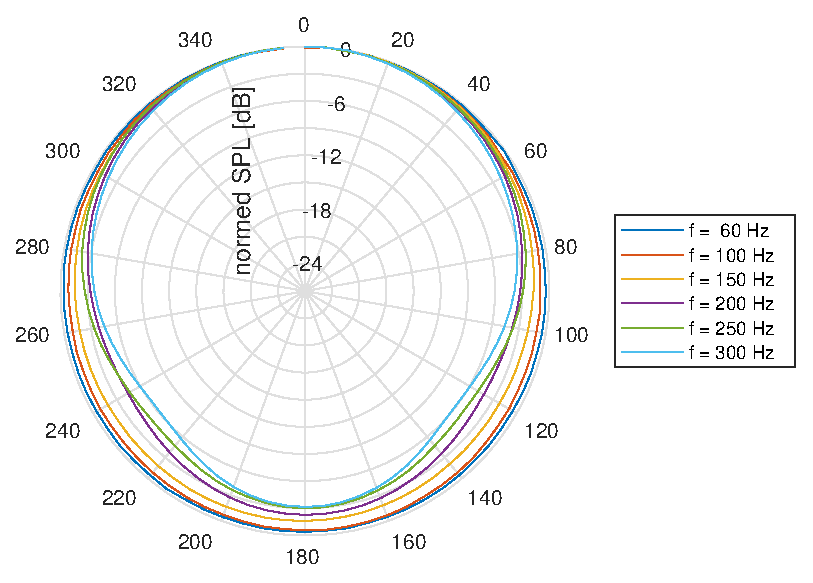
\includegraphics[width=0.7\textwidth]{03_02_meas1_pressure.eps}
	\caption{Normed \gls{spl}, measured at a distance \(d=\)\SI{2.74}{\meter}}
		\label{fig:03_02_m1_pressure}
\end{figure}
\autoref{fig:03_02_m1_phase} visualizes the phase in an angular range from \SI{-180}{\degree} to \SI{180}{\degree} phase angle. Values outside of this range have been shifted by integer multiples of \SI{360}{\degree}. Similar to \autoref{fig:03_02_m1_pressure}, the graphs up to a  frequency of \SI{150}{\hertz} have a near-circular shape. The circles are also slightly offset towards the \SI{0}{\degree} direction. At higher frequencies, the shape gradually changes towards something closer to a cardiod.
As indicated  by the non-concentric graphs and the calculation in \autoref{sec:ac_center}, the acoustic center of the loudspeaker still seems to be in front of the rotational axis by some margin. To move it back the calculated distance, changes to the mechanical support system have to be implemented and another measurement has to be conducted.
\begin{figure}[htbp]
	\centering
	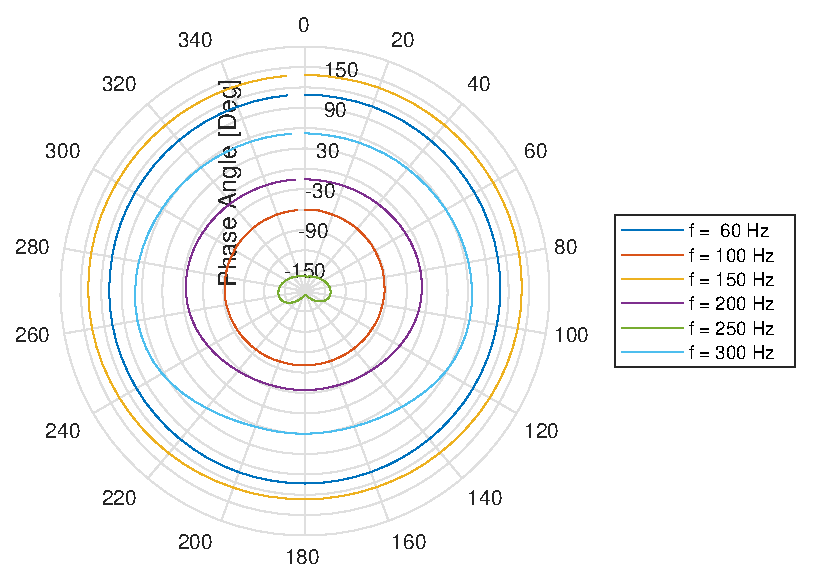
\includegraphics[width=0.7\textwidth]{03_02_meas1_phase.eps}
	\caption{Phase, measured at a distance \(d=\)\SI{2.74}{\meter}}
		\label{fig:03_02_m1_phase}
\end{figure}



\chapter{Measurement of Directional Characteristics III}\label{ax:directional_3}
This appendix serves as a protocol to a series of measurements conducted between the 10\textsuperscript{th} and 12\textsuperscript{th} of May  2018 in the large anechoic chamber (B4-111) at the acoustic lab of Aalborg University at Fredrik Bajers Vej 7.\\
The goal of these measurements is investigating the behaviour of a loudspeaker array consisting of three of the loudspeakers that have been featured in \autoref{ax:directional_1} and \ref{ax:directional_2}.

\section*{Measuring Equipment and Materials}
The following measuring equipment was used:
\begin{itemize}[noitemsep]
\item Microphone \gls{bandk} 4144
\begin{itemize}[noitemsep]
\item AAU-number: 06552
\item Serial number: 297090
\end{itemize}
\item Preamplifier GRAS 26AK
\begin{itemize}[noitemsep]
\item AAU-number: 56526
\item Serial number: 32810
\end{itemize}
\item Power supply \gls{bandk} 2636
\begin{itemize}
\item AAU-number: 08022
\item Serial number: 
\end{itemize}
\item Calibrator \gls{bandk}\ 4231
\begin{itemize}[noitemsep]
\item AAU-number: 33691
\item Serial number: 2115338
\end{itemize}
\item 2 pcs. Power Amplifier Pioneer A-616
\begin{itemize}[noitemsep]
\item AAU-number: 08249, 08699
\item Serial number: HJ9404841S, JG9405804S
\end{itemize}
\item Sound card RME Fireface UCX
\begin{itemize}[noitemsep]
\item AAU-number: 108230
\item Serial number: 23811948
\end{itemize}
\item Turntable: Outline ET 250-3D
\begin{itemize}
\item Serial number: REIB0012
\end{itemize}
\item MATLAB r2017b on OSX 10.11.6
\item 3 pcs. Loudspeaker SEAS 33 F-WKA
\end{itemize}

The following material was used:
\begin{itemize}[noitemsep]
%\item \SI{1/2}{\inch} to \SI{1}{\inch} preamp adapter
\item Microphone clip
\item Microphone stand
\item LEMU cable
\item \gls{bandk} cable
\item XLR cables
\item Ethernet cable
\item miscellanious adapters
\item 3 pcs. Loudspeaker cabinet, plywood, outside dimensions: (400x400x400)\SI{}{\milli\meter}, wall~thickness:~\SI{20}{\milli\meter}, equipped with \citep{seas33}
\item Speaker mount for turntable
\begin{itemize}[noitemsep]
\item Steel mounting contraption, see REFERENCE TO HARDWARE CHAPTER
\item 3 speaker legs, \SI{40}{\milli\meter} box section, top: aluminium, {\(\varnothing\)~:~\SI{34.8}{\milli\meter}}, height: \SI{1}{\meter}
\item Circular \gls{mdf} cutout, thickness: \SI{12}{\milli\meter}, {\(\varnothing\)~:~\SI{800}{\milli\meter}}
\item \gls{mdf} cutout, thickness: \SI{20}{\milli\meter}, surface: approx. (300x600)\SI{}{\milli\meter}, bolt pattern drilled according to the bottom side of the ET 250-3D turntable
\item \gls{mdf} cutout for counterweight mounting, thickness: \SI{12}{\milli\meter}, surface : (400x400)\SI{}{\milli\meter}
\item triangular cutout (isosceles), thickness: \SI{12}{\milli\meter}, approximate outside dimensions (base width x height): (970x600)\SI{}{\milli\meter}
\item 2 Electrovoice S-200 speakers as counterweight
\item Ratchet strap
\item 4 bolts M8x80, associated washers
\item 6 bolts M8x30, associated washers
\item 8 sinkhead bolts M8x40, associated nuts and washers
\item miscellaneous woodscrews

\end{itemize}
\end{itemize}



\section*{Setup}\label{sec:05_11_setup}
When setting up the speaker array according to dimensions that have been decided upon in \autoref{sec:opt_result}, a substential effort was undertaken to insure a secure stance. The turntable was mounted to one of the platform grids used in the anechoic chamber by screwing bolts through a \gls{mdf}-plate and the grid into the threads on the underside of the turntable. A round \gls{mdf} plate was mounted using the boltpattern on the upside of the turntable. Fixed to the round plate the custom made steel contraption (see \autoref{sec:hardware}) was bolted, which itself held the legs of the speakers in place. while allowing some adjustability. In a height of approx \SI{1}{\meter} above the turntable the three speaker cabinets were mounted to the legs. On top of the speaker a triangular \gls{mdf} cutout was employed to enhance rigidity. A picture of the array is given in \autoref{fig:05_11_setup}.

\begin{figure}[h]\label{fig:05_11_setup}
	\centering
    \includegraphics[width=0.5\textwidth]{05_11_setup.jpg}
    \caption{Speaker array setup on the turntable in the anechoic chamber.}
\end{figure}

The height of the centers of the speaker cabinet above the grid turned out to be \SI{1.37}{\meter}. The microphone was set up in the same height. Platforms for the speaker array and the microphone were set up in opposing corners of the anechoic chamber, which resulted in a horizontal distance between the array center and the microphone of \SI{4.92}{\meter}.
The input and the output gain of the \gls{bandk} 2636 microphone power supply were both set to \SI{+10}{\decibel}. The input gain on the Fireface UCX was set to \SI{0}{\decibel}. On the playback side, the power amplifiers had a fixed voltage gain of \SI{+10}{\decibel} and the \texttt{playgain}-parameter in the measurement routine was set to \SI{-10}{\decibel}. The playback signals were normed so that the absolute of the biggest amplitude in on of the filtered sweeps (see \autoref{sec:filter_design} is a digital value of 1.\\
The desired positioning of the acoustic centers of the speakers was found to be describable as \texttt{Lx}$\,=\,\SI{40}{\centi\meter}$ and \texttt{Ly}$\,=\,\SI{-40}{\centi\meter}$ in \autoref{sec:opt_result}. In order to make achieve the positioning without the loudspeaker cabinets physically interfering, the azimuth of both of the two front loudspeakers \texttt{B} and \texttt{C} was rotated by \SI{50}{\degree} inwards. The speaker positions were adjusted according to the finding of \autoref{ax:directional_2}, that the acoustic center of the speaker is approx. \SI{17}{\centi\meter}. The array center was set on the rotational axis of the turntable, in order to match the way, the point sources are set up in the analytical model and the \gls{fdtd} simulation.
This positioning was used as a baseline for measurements and was later adjusted to account for imprecisions and assymetries in the way the speakers were set up and further tweaked with an heuristic approach to changing the positions in order to achieve the best possible result with the given hardware and without changing the \gls{sp}-parameters. It is assumed that these tweeks were necessary in order to account for the influence that the speaker cabinets had on the sound field. By the time of the final measurements, the rear speaker \texttt{A} had been moved towards the front by \SI{4.5}{\centi\meter}, the side speakers had been moved towards the inside by \SI{2}{\centi\meter} each, and their azimuth angle had been increased to approx. \SI{55}{\degree}.
To illustrate the way, the speakers were set up, a birdseye view is given in \autoref{fig:array_pic}.
\begin{figure}[h]
	\centering
    \includegraphics[width=0.5\textwidth]{speaker_array.jpg}
    \label{fig:array_pic}
    \caption{Speaker array arrangement}
\end{figure}

\section*{Results}\label{sec:05_11_results}
In the course of the measurement campaign, numerous polar responses have been measured. The main assessment on how the results are to be interpreted in the context of the overall project can be found in REFERENCE TO MAIN CHAPTER.\\
For this appendix, only an overview over the measured data is given.
The first measurement that was conducted, the polar response of the beamforming array with the speaker cabinets arranged in the inital positioning was recorded. The results are shown in \autoref{fig:05_11_initial}.
\begin{figure}[h]
\begin{subfigure}[c]{0.5\textwidth}
\includegraphics[width=0.85\textwidth]{05_11_initial_pr.eps}
\subcaption{Pressure}
\label{fig:05_11_init_pr}
\end{subfigure}
\begin{subfigure}[c]{0.5\textwidth}
\includegraphics[width=0.95\textwidth]{05_11_initial_ph.eps}
\subcaption{Phase}
\label{fig:05_11_init_ph}
\end{subfigure}\\
\caption{Polar response, initial positioning}  
\label{fig:05_11_initial}
\end{figure}
Additional to verifying the beamforming capabilities of the array itself in combination with the chosen parameter set, the polar responses of each of the speakers has been measured, by disabling all signal processing that is related to the beamforming and disabling playback on the all but the measured speaker. The information gained in these measurements allows for verifying the symmetry of the setup as well as estimating the relative position of the acoustic in relation to the rotational axis of the turntable, which also is defined to be the array center. Also, more sophisticated pressure and phase correctional tables for the parameter optimization could be derived, if further development of the array is desired. The results are displayed in \autoref{fig:05_11_single}. These measurements were conducted with the speaker positioning, that had been adjusted as described in \autoref{sec:05_11_setup}.
The graphs can be compared with those displayed in \autoref{fig:03_02_m1_pressure} and \ref{fig:03_02_m1_phase}, which were measured with only a single speaker. The position of the speakers in the array is different in terms of distance of the acoustical center to the rotational axis of the turntable and the relation of the main axis of the speaker in terms of angle to the zero degree position of the turntable. If there was no significant influence of the speaker cabinets in the array on the directional characteristics of the individual speakers, all of the formerly mentioned graphs would only differ by a minimal shift of similar shapes in relation to the pole and in rotation. 
However, significant differences in the the shape of the graphs are apparent, e.g. when looking at \SI{250}{\hertz}-phase graphs. This indicates, that there is an influence of the speaker cabinets in the array on the way, sound emerges from the loudspeakers. The significance of this influence appears to be frequency dependent. The shape of the \SI{60}{\hertz} and \SI{100}{\hertz} graphs is close to circular in all of the measurements.

\begin{figure}[h]
\begin{subfigure}[c]{0.5\textwidth}
\includegraphics[width=0.85\textwidth]{05_11_A_pr.eps}
\subcaption{Speaker A, pressure}
\label{fig:05_11_A_pr}
\end{subfigure}
\begin{subfigure}[c]{0.5\textwidth}
\includegraphics[width=0.95\textwidth]{05_11_A_ph.eps}
\subcaption{Speaker A, phase}
\label{fig:05_11_A_ph}
\end{subfigure}\\
\hspace{0.1\textheight}
\begin{subfigure}[c]{0.5\textwidth}
\includegraphics[width=0.85\textwidth]{05_11_B_pr.eps}
\subcaption{Speaker B, pressure}
\label{fig:05_11_A_pr}
\end{subfigure}
\begin{subfigure}[c]{0.5\textwidth}
\includegraphics[width=0.95\textwidth]{05_11_B_ph.eps}
\subcaption{Speaker B, phase}
\label{fig:05_11_A_ph}
\end{subfigure}\\
\hspace{0.1\textheight}
\begin{subfigure}[c]{0.5\textwidth}
\includegraphics[width=0.85\textwidth]{05_11_C_pr.eps}
\subcaption{Speaker C, pressure}
\label{fig:05_11_A_pr}
\end{subfigure}
\begin{subfigure}[c]{0.5\textwidth}
\includegraphics[width=0.95\textwidth]{05_11_C_ph.eps}
\subcaption{Speaker C, phase}
\label{fig:05_11_A_ph}
\end{subfigure}\\
\caption{Polar responses of each speakers alone, final positioning}  
\label{fig:05_11_single}
\end{figure}

Another measurement has been conducted, where all three speakers in the array played back the same signal. This means no beamforming was taking place. The results are displayed in \autoref{fig:05_11_all}. As well as serving as a baseline to how much attenuation is actually achieved by beamforming, this measurement can also provide a hint on weather the definition of the array center in \autoref{sec:genetic_implementation} has been a reasonable choice.
In \label{sec:ac_center}, the acoustic center has been established as the point in space, from which a virtual point source emitts sound. The conclusion from this is, that, when the acoustic center is placed on the rotational axis of the turntable during measurements, the resulting graphs in the polar plots of pressure and phase are circular and concentrical - just like the \SI{60}{\hertz} and \SI{100}{\hertz} pressure and phase graphs from the formerly mentioned measurement. 
Two things can be concluded from this. Firstly, placing the acoustic centers of a speaker array in a triangle leads to the centroid of this triangle acting as the acoustical center of the array, when all speakers play the same signal, which makes the decision to treat this position as the array center reasonable. Secondly, the adjustments, that have been made to the initial positions as described in \autoref{sec:05_11_setup}, have lead to positions of the acoustic centers, that are close to the desired positions.

\begin{figure}[h]
\begin{subfigure}[c]{0.5\textwidth}
\includegraphics[width=0.85\textwidth]{05_11_all_pr.eps}
\subcaption{Pressure}
\label{fig:05_11_all_pr}
\end{subfigure}
\begin{subfigure}[c]{0.5\textwidth}
\includegraphics[width=0.95\textwidth]{05_11_all_ph.eps}
\subcaption{Phase}
\label{fig:05_11_all_ph}
\end{subfigure}\\
\caption{Polar response of the speaker array, beamforming disabled, final positioning}  
\label{fig:05_11_all}
\end{figure}

The directional characteristics of the speaker array with its final, adjusted positioning and the beamforming enabled by using filtering as described in \autoref{sec:filter_design} are shown in \autoref{fig:05_11_final}. A significant improvement over the characteristic with the inital positioning displayed in \autoref{fig:05_11_inital} has been achieved at the \SI{180}{\degree} direction. The attenuation compared to the main axis at this direction is bigger or equal to approx. \SI{12}{\decibel} at all frequencies. The maximum \SI{-3}{\decibel}-lobe width is approx. \SI{140}{\degree}, the maximum \SI{-3}{\decibel}-lobe width is approx. \SI{200}{\degree}. The phase graphs have a clearly non-circular shape. At roughly \SI{140}{\degree} and \SI{-140}{\degree} there are jumps in the phase graphs, between an approximately circular phase curve towards the main axis of the array and a phase shifted by anything between \SI{110}{\degree} and \SI{220}{\degree} compared to the front section.

\begin{figure}[h]
\begin{subfigure}[c]{0.5\textwidth}
\includegraphics[width=0.85\textwidth]{05_11_final_pr.eps}
\subcaption{Pressure}
\label{fig:05_11_final_pr}
\end{subfigure}
\begin{subfigure}[c]{0.5\textwidth}
\includegraphics[width=0.95\textwidth]{05_11_final_ph.eps}
\subcaption{Phase}
\label{fig:05_11_final_ph}
\end{subfigure}\\
\caption{Polar response of the speaker array with beamforming, final positioning}  
\label{fig:05_11_final}
\end{figure}
\chapter*{Transfer function measurement software}
In this appendix the transfer function software will be briefly explained. The gold of this software is to be able to compute the impulse response of a \gls{dut} using the logarithmic swept sine method and then compute the transfer function from the impulse response. To be able to send out a logarithmic swept sine and measure it, a full duplex soundcard have to be chosen and used as the measuring soundcard. To be able to reproduce all measurement and compare other measurement, the soundcard will not be changed doing the project work.

\section*{Materials and setup}
To measure transfer function of a \gls{dut}, the following materials are used:
\begin{itemize}
\item RME FIREFACE ucx (Soundcard)
\item MATLAB (PC - software)
\end{itemize}

\begin{figure}[htbp!]
\centering
\def\svgwidth{\columnwidth}
\chapter{Test of the Guitar's Frequency Area}\label{app:frequency_area}
A test was made to get an overview of the frequency area in which the tones from the guitar lie.

\section*{Materials and Setup}
To measure the frequency area on a guitar, the following materials are used:
\begin{itemize}
\item Digilent Analog Discovery 2 (Oscilloscope)
\item Fender Squier Classic Vibe Telecaster (Guitar)
\item Digilent Waveforms 2015 (PC - software)
\end{itemize}

\begin{figure}[htbp!]
\centering
\def\svgwidth{\columnwidth}
\input{figures/appendix/guitar_frequency_test.pdf_tex}
\caption{Setup for measuring frequency area on a guitar.}
		\label{fig:appendix:guitar_freq}
\end{figure}

\section*{Test Procedure}
To measure the frequency area on a guitar, the following steps are followed:
\begin{enumerate}
\item The materials are set up as in \autoref{fig:appendix:guitar_freq}.
\item Digilent Waveforms 2015 is set as a spectrum analyser. 
\item The guitar is set to use the neck pickup, the volume and tone control are turned all the way up to their maximum.
\item The highest and the lowest tone on the guitar are played, measured by the oscilloscope and analysed in Digilent Waveforms 2015.
\item The guitar is set to use the bridge pickup and step 4 is repeated. 
\item The data is plotted in MATLAB.
\end{enumerate}

\section*{Results}

\begin{figure}[htbp!]
	\centering
		\includegraphics[width=1\textwidth]{guitar_low_E_neck.pdf}
		\caption{Measurement of the low E note on the neck pickup.}
		\label{fig:appendix:low_E_neck}
\end{figure}

On \autoref{fig:appendix:low_E_neck} it is seen that the lowest significant frequency is around \SI{80}{\hertz} and the highest significant frequency is around \SI{500}{\hertz}, when playing the low E note on the guitar, using the neck pickup.

\newpage
\begin{figure}[htbp!]
	\centering
		\includegraphics[width=1\textwidth]{guitar_low_E_bridge.pdf}
		\caption{Measurement of the low E note on the bridge pickup.}
		\label{fig:appendix:low_E_bridge}
\end{figure}

On  \autoref{fig:appendix:low_E_bridge} it is seen that the lowest significant frequency is around \SI{80}{\hertz} and the highest significant frequency is around \SI{730}{\hertz}, when playing the low E note on the guitar, using the bridge pickup.

\begin{figure}[htbp!]
	\centering
		\includegraphics[width=1\textwidth]{guitar_high_Cis_neck.pdf}
		\caption{Measurement of the high C\# note on the neck pickup.}
		\label{fig:appendix:high_Cis_neck}
\end{figure}

On  \autoref{fig:appendix:high_Cis_neck} it is seen that the lowest significant frequency is around \SI{1100}{\hertz} and the highest significant frequency is around \SI{4400}{\hertz}, when playing the high C\# note on the guitar, using the neck pickup.

\newpage
\begin{figure}[htbp!]
	\centering
		\includegraphics[width=1\textwidth]{guitar_high_Cis_bridge.pdf}
		\caption{Measurement of the high C\# note on the bridge pickup.}
		\label{fig:appendix:high_Cis_bridge}
\end{figure}

On  \autoref{fig:appendix:high_Cis_bridge} it is seen that the lowest significant frequency is around \SI{1100}{\hertz} and the highest significant frequency is around \SI{4400}{\hertz}, when playing the high C\# note on the guitar, using the bridge pickup. 

\begin{figure}[htbp!]
	\centering
		\includegraphics[width=1\textwidth]{guitar_high_E_flasholet_bridge.pdf}
		\caption{Measurement of the high E note, played as flasholet, on the bridge pickup.}
		\label{fig:appendix:high_E_bridge_flasholet}
\end{figure}

On  \autoref{fig:appendix:high_E_bridge_flasholet} it is seen that the lowest significant frequency is around \SI{1300}{\hertz} and the highest significant frequency is around \SI{2600}{\hertz}, when playing the high E note on the guitar as flasholet, using the bridge pickup. 

\caption{Setup for measuring frequency area on a guitar.}
		\label{fig:appendix:test}
\end{figure}

\section*{Test procedure}


\begin{enumerate}
\item The materials are set up as in \autoref{fig:appendix:test}.
\item 
\item  
\item  
\item 
\item 
\end{enumerate}

\section*{Results}

\begin{figure}[htbp!]
	\centering
		\includegraphics[width=1\textwidth]{guitar_low_E_neck.pdf}
		\caption{Measurement of the low E note on the neck pickup.}
		\label{fig:appendix:low_E_neck}
\end{figure}

On  \autoref{fig:appendix:low_E_neck} it is seen that the lowest significant frequency is around \SI{80}{\hertz} and the highest significant frequency is around \SI{400}{\hertz}, when playing the low E note on the guitar, using the neck pickup.


\chapter*{Frequency response of RME FIREFACE UCX}\label{Frequency_response_of_RME_FIREFACE_UCX}
A test was made to get a view of the frequency response of the RME FIREFACE ucx. The RME FIREFACE ucx is used for all measurement in this project, and therefore the frequency response is of interest. To measure the frequency response, the function from \autoref{appendix:transfer_function} is used.

\section*{Materials and setup}
To measure the frequency response of the RME FIREFACE UCX, the following materials are used:
\begin{itemize}
\item RME FIREFACE ucx (Soundcard)
\begin{itemize}[noitemsep]
\item AAU-number: 108230
\item Serial number: 23811948
\end{itemize}
\item MATLAB 2017b (PC - Software)
\item IRmeas_fft (software) \autoref{appendix:transfer_function}
\item jack to jack cable
\end{itemize}

\begin{figure}[H]
\centering
\begin{picture}(0,0)%
\includegraphics{rme_transfer_function.pdf}%
\end{picture}%
\setlength{\unitlength}{2818sp}%
%
\begingroup\makeatletter\ifx\SetFigFont\undefined%
\gdef\SetFigFont#1#2#3#4#5{%
  \reset@font\fontsize{#1}{#2pt}%
  \fontfamily{#3}\fontseries{#4}\fontshape{#5}%
  \selectfont}%
\fi\endgroup%
\begin{picture}(4090,4926)(8176,-7474)
\put(8191,-3661){Out}%
\put(9271,-3211){Sound Card}%
\put(9971,-6361){Computer}%
\put(11836,-4696){USB}%
\put(8281,-2806){In}%
\end{picture}%
\caption{Setup for measuring transfer function}
		\label{fig:appendix:rme_response}
\end{figure}

\section*{Test procedure}


\begin{enumerate}
\item The materials are set up as in \autoref{fig:appendix:rme_response}.
\item The cable is connected between input 1 and output 1
\item The input gain at input 1 is set to \SI{20}{\decibel}
\item The output \texttt{playgain} is set to \SI{-18}{\decibel}
\item The input and output channel is specified in the MATLAB function "SynchronizedPlaybackAcquirer" 
\item IRmeas_fft (software) \autoref{appendix:transfer_function} is preformed
\item The transfer function is plotted from \SI{20}{\hertz} to \SI{20}{\kilo\hertz}
\end{enumerate}

\section*{Results}



On \autoref{fig:appendix:rme_response_result} it is seen that the soundcard only have a non linearity of \SI{0.26}{\decibel} from \SI{20}{\hertz} to \SI{20}{\kilo\hertz} between output data and input data. 

\begin{figure}[H]
	\centering
	\includegraphics[width=1\textwidth]{RME_FIREFACE_UCX_tf.pdf}
	\caption{The frequency response of the RME FIREFACE UCX with input sensitivity at 20}
		\label{fig:appendix:rme_response_result}
\end{figure}

\section*{Conclusion}
It can be concluded that en RME_FIREFACE_UCX have a non linearity of \SI{0.26}{\decibel} when the input gain is at \SI{20}{\decibel} and the output \texttt{playgain} is at \SI{-18}{\decibel}



\chapter{Frequency response of Pioneer A-616}
A test was made to assess the frequency response of a Pioneer A-616 amplifier. The Pioneer A-616 amplifier is used for all the polar response measurements in this project, and therefore the frequency response has to be investigated. To measure the frequency response, the function from \autoref{appendix:transfer_function} is used. The test is executed with and without load, to investigate, whether the load affects the transfer function of the amplifier.

\section*{Materials and setup}
To measure the frequency response of the Pioneer A-616 amplifier, the following materials are used:
\begin{itemize}
\item RME FIREFACE UCX (Soundcard)
\begin{itemize}[noitemsep]
\item AAU-number: 108230
\item Serial number: 23811948
\end{itemize}
\item Pioneer A-616 with a maximum voltage gain of \SI{44}{\decibel} (amplifier)
\begin{itemize}[noitemsep]
\item AAU-number: B4-109-C-8
\item Serial number: HJ9404841S
\end{itemize}
\item MATLAB 2017b (PC - Software)
\item IRmeas_fft (software) \autoref{appendix:transfer_function}
\item SEAS 33 F-WKA mounted in an enclosed 
\item XLR speaker cable
\item Jack to phone signal cable
\item Jack to banana cable
\end{itemize}

\begin{figure}[H]
\centering
\begin{picture}(0,0)%
\includegraphics{pioneer_transfer_function.pdf}%
\end{picture}%
\setlength{\unitlength}{2818sp}%
%
\begingroup\makeatletter\ifx\SetFigFont\undefined%
\gdef\SetFigFont#1#2#3#4#5{%
  \reset@font\fontsize{#1}{#2pt}%
  \fontfamily{#3}\fontseries{#4}\fontshape{#5}%
  \selectfont}%
\fi\endgroup%
\begin{picture}(8338,4926)(3838,-7474)
\put(9991,-6361){Computer}%
\put(6661,-6091){Amplifier}%
\put(9271,-3211){Sound Card}%
\put(11746,-4696){USB}%
\put(8236,-3526){Out}%
\put(8281,-3031){In}%
\put(3961,-4336){Loudspeaker}%
\put(5131,-5371){Switch}%
\end{picture}%
\caption{Setup for measuring transfer function}
		\label{fig:appendix:pioneer_response}
\end{figure}

\section*{Test procedure}


\begin{enumerate}
\item The materials are set up as in \autoref{fig:appendix:pioneer_response}.
\item The signal cable is connected between the RME FIREFACE UCX output channel 1 and right Line input on the amplifier.
\item The jack to banana cable is connected between the amplifier right B output channel to the  RME FIREFACE UCX input 1 
\item The input gain of RME FIREFACE UCX at input 1 is set to \SI{20}{\decibel}
\item The input and output channel is specified in the MATLAB function "SynchronizedPlaybackAcquirer" 
\item NOTE! the following two step is preformed in parallel, so the volume nob stays the same for every attenuation. The attenuation is controlled by a volume nob in front of the amplifier.
\item IRmeas_fft (software) \autoref{appendix:transfer_function} is preformed with attenuation of \SI{-40}{\decibel}, \SI{-16}{\decibel}  and  \SI{0}{\decibel} of the amplifier without load 
\item then IRmeas_fft (software) \autoref{appendix:transfer_function} is preformed with attenuation of \SI{-40}{\decibel}, \SI{-16}{\decibel} and \SI{0}{\decibel} of the amplifier with load. 
\item the measurement is done with \texttt{playgain} \SI{-18}{\decibel}, \SI{-42}{\decibel} and \SI{-57}{\decibel} respectively, so the output voltage of the amplifier do not damage the soundcard.
\item The measured transfer function from the RME FIREFACE UCX is compensated in all measurements, to get a unaffected voltage gain of the amplifier.
\item The transfer function is plotted from \SI{20}{\hertz} to \SI{20}{\kilo\hertz} for every measurement, where the measurement with load is plotted first in read, and then the measurement without load is plotted in blue.

\end{enumerate}

\section*{Results}



Regarding \autoref{fig:appendix:amplifier_response_result} it is apparent, that the influence of the output load, as which the SEAS 33 F-WKA speaker acts, on the transfer function of the amplifier is negligible. The red and blue curves match up at all three measured levels. The amplifier can not be represented as a linear gain factor from \SI{20}{\hertz} to \SI{20}{\kilo\hertz} at high attenuation, because the deviation from a linear frequency response at a playback level of \SI{-40}{\decibel} on the amplifier is \SI{1.75}{\decibel} from the highest to the lowest attenuation. The amplifier works more like a linear gain factor when the attenuation is lowered. The deviation from a linear frequency response at an attenuation of \SI{0}{\decibel} is \SI{0.16}{\decibel}. At \SI{-16}{\decibel} the deviation is \SI{0.55}{\decibel}.



\begin{figure}[H]
	\centering
	\includegraphics[width=1\textwidth]{transfer_function_of_amplifier.pdf}
	\caption{The frequency response of the Pioneer A-616 there the lower blue and red curve display the attenuation of \SI{-40}{\decibel}. The middle blue and red curve correspond to an attenuation of \SI{-16}{\decibel} and the upper blue and red curve correspond to an attenuation of  \SI{0}{\decibel}}
		\label{fig:appendix:amplifier_response_result}
\end{figure}

\section*{Conclusion}
It can be concluded that the transfer function of the amplifier Pioneer A-616 does not significantly depend on a load on the output. It can also be concluded that the amplifier can be represented as a gain factor from \SI{20}{\hertz} to \SI{20}{\kilo\hertz} with attenuation smaller than \SI{-16}{\decibel}, because a deviation of \SI{0.55}{\decibel} or lower is accepted.


\chapter{Microphone calibration software} \label{appendix:calibration}
In this appendix the microphone calibration software will be briefly explained. The goal of this software is to be able to calibrate any microphone including the calibration of the soundcard in MATLAB, so that a calibration tone corresponds to a known digital number in MATLAB. 

\section*{Materials and setup}
To do a calibration of a arbitrary microphone, the following materials are used:
\begin{itemize}
\item RME FIREFACE UCX (Soundcard)
\begin{itemize}[noitemsep]
\item AAU-number: 108230
\item Serial number: 23811948
\end{itemize}
\item E.g. \gls{bandk} TYPE 4231 (calibrator )
\begin{itemize}[noitemsep]
\item AAU-number: 33691
\item Serial number: 2115338
\end{itemize}
\item MATLAB 2017b (PC - software)
\item Random microphone 
\item XLR signal cable
\end{itemize}


\paragraph{The first step}

\begin{figure}[H]
\centering
\begin{picture}(0,0)%
\includegraphics{rme_transfer_function.pdf}%
\end{picture}%
\setlength{\unitlength}{2818sp}%
%
\begingroup\makeatletter\ifx\SetFigFont\undefined%
\gdef\SetFigFont#1#2#3#4#5{%
  \reset@font\fontsize{#1}{#2pt}%
  \fontfamily{#3}\fontseries{#4}\fontshape{#5}%
  \selectfont}%
\fi\endgroup%
\begin{picture}(4090,4926)(8176,-7474)
\put(8191,-3661){Out}%
\put(9271,-3211){Sound Card}%
\put(9971,-6361){Computer}%
\put(11836,-4696){USB}%
\put(8281,-2806){In}%
\end{picture}%
\caption{Setup for calibrating the soundcard}
		\label{fig:appendix:rme_calibration}
\end{figure}

\paragraph{The second step}

\begin{figure}[H]
\centering
\begin{picture}(0,0)%
\includegraphics{mic_calibration.pdf}%
\end{picture}%
\setlength{\unitlength}{2818sp}%
%
\begingroup\makeatletter\ifx\SetFigFont\undefined%
\gdef\SetFigFont#1#2#3#4#5{%
  \reset@font\fontsize{#1}{#2pt}%
  \fontfamily{#3}\fontseries{#4}\fontshape{#5}%
  \selectfont}%
\fi\endgroup%
\begin{picture}(7944,6816)(3679,-7474)
\put(10036,-6361){Computer}%
\put(4951,-1771){Microphone}%
\put(6661,-1501){Amplifier}%
\put(9271,-3211){Sound Card}%
\put(8171,-3096){In}%
\put(8171,-3626){Out}%
\put(3961,-2941){Calibrator}%
\put(11746,-4606){USB}%
\end{picture}%
\caption{Setup for calibrating the microphone}
		\label{fig:appendix:mic_calibration}
\end{figure}

\section*{The calibration step} \label{apendix:calibrate_sound_card_and_microphone}
\paragraph{The first step} is measuring the transfer function of the sound card according to \autoref{Frequency_response_of_RME_FIREFACE_UCX} and the set up is shown is \autoref{fig:appendix:rme_calibration}. The complex transfer function is divided by the input of the sound card, such that the gain between input and output of the sound card is 1 from \SI{20}{\hertz} to \SI{20}{\kilo\hertz}, when a signal cable is connected between input and output. While doing the calibration, the peak value at the input is saved and used as a reference value of the sound card. All measurement have to include the calibration of the sound card, to ensure that a known digital number in MATLAB correspond to a known pressure.
\paragraph{The second step} is measuring the digital number in MATLAB that corresponding to \SI{1}{\pascal} or \SI{94}{\decibel} and then log value as the microphone calibration peak value. The set up is shown is \autoref{fig:appendix:mic_calibration}. The factor between reference value of the sound card divided by the microphone calibration correspond to the factor that have to be multiplied to the input of the sound card, and only works with the microphone used in the calibration. This calibration have to be done before every series of measurement. The function will return the digital number 1 when the pressure is \SI{1}{\pascal} and is linearly depending on the pressure. To calculate the \gls{spl} the following formula is used

\begin{equation}
dB\,\, re. \SI{20}{\micro\pascal} = 20 \cdot log_{10} \left ( \frac{p}{p_0} \right )
\end{equation}

    \startexplain
    		\explain{$p$ is the returned number from the function }{\si{\pascal}}
        \explain{$p_0$ is the reference pressure}{\si{\pascal}}
    \stopexplain  


\section*{The MATLAB function for measuring the input}
To ensure that the calibration and measuring record software is as identical as possible, the same function is used just modified so instead of playing a swept sine, it will play a string of zero.

\section*{The MATLAB function}
\includeCode{irmeas_fft_mic.m}{matlab}{1}{40}{The calibration record software}{code:irmeas_fft_mic}{./code/microphone_calibration/sine_sweep/}




\chapter{Measuring the output voltage of RME FIREFACE UCX}
A test was made to get a view of the output voltage of the sound card and its corresponding digital value. The test will be done with a continues \SI{1}{\kilo\hertz} tone, because the all measurement will be done with calibrated sound card and in the area of the amplifier, where the transfer function is linear.

\section*{Materials and setup}
To measure the output voltage, the following materials are used:
\begin{itemize}
\item Digilent Analog Discovery 2 (Oscilloscope)
\begin{itemize}[noitemsep]
\item AAU-number: 2179-12
\item Serial number: DA3716C
\end{itemize}
\item RME FIREFACE ucx (Soundcard)
\begin{itemize}[noitemsep]
\item AAU-number: 108230
\item Serial number: 23811948
\end{itemize}
\item Digilent Waveforms 2015 (PC - software)
\item MATLAB 2017b (PC - software)
\item SynchronizedPlaybackAcquirer, where \texttt{playgain} is the output attenuation in \si{\decibel} (Made by MATLAB)
\end{itemize}

\begin{figure}[htbp!]
\centering
\begin{picture}(0,0)%
\includegraphics{RME_voltage_out.pdf}%
\end{picture}%
\setlength{\unitlength}{2818sp}%
%
\begingroup\makeatletter\ifx\SetFigFont\undefined%
\gdef\SetFigFont#1#2#3#4#5{%
  \reset@font\fontsize{#1}{#2pt}%
  \fontfamily{#3}\fontseries{#4}\fontshape{#5}%
  \selectfont}%
\fi\endgroup%
\begin{picture}(5212,4926)(6964,-7474)
\put(10036,-6361){Computer}%
\put(9271,-3211){Sound Card}%
\put(8171,-2996){In}%
\put(8171,-3526){Out}%
\put(7831,-5056){In}%
\put(5431,-5856){Oscilloscope}%
\put(8236,-6676){USB}%
\put(11746,-4606){USB}%
\end{picture}%
\caption{Setup for measuring output voltage of the sound card.}
		\label{fig:appendix:rme_output_voltage}
\end{figure}

\section*{Test procedure}


\begin{enumerate}
\item The materials are set up as in \autoref{fig:appendix:rme_output_voltage}.
\item A sinusoid with a frequency of \SI{1}{\kilo\hertz} and a digital amplitude of 1 is created.  
\item The sinusoid is played continuously at the output of the sound card with a \texttt{playgain} of  \SI{0}{\decibel}.
\item  A measurement of the sinusoid on the output of the sound card is made with Digilent Analog Discovery 2.
\item The data from Digilent Analog Discovery 2 is imported to MATLAB and plotted with the sinusoid created in MATLAB
\end{enumerate}

\section*{Results}

\begin{figure}[htbp!]
	\centering
		\includegraphics[width=1\textwidth]{rme_output_voltage.pdf}
		\caption{The output voltage compare to the digital value in MATLAB}
		\label{fig:appendix:rme_output_voltage_result}
\end{figure}

On  \autoref{fig:appendix:rme_output_voltage_result} it is seen that the digital number 1 in MATLAB corresponding to a voltage of \SI{4.7}{\volt} when the \texttt{playgain} is at \SI{0}{\decibel}. 

\section*{Conclusion}
It can be concluded that the factor between the digital number in MATLAB and the output voltage is 4.7 with \texttt{playgain} of \SI{0}{\decibel}. Since the sound card will be calibrated for every measurement, it is concluded that this factor is linear from \SI{20}{\hertz} to \SI{20}{\kilo\hertz}. 




\chapter{Speaker measuring manual} \label{appendix:measuring_manual}
In this appendix the polar response measurement software will be briefly explained. The gold of this software is to measure the polar response and calculate the transfer function of any loudspeaker in the anechoic chamber, with calibrated measuring tools. polar response is an impulse response measurement for every specified degree step size around the speaker. E.g. if the step is one degree, the loudspeaker will be turned 1 degree for every  impulse response measurement, until \SI{360}{\degree} is achieved.

\section*{Materials and setup}
To measure the \SI{360}{\degree} transfer function of a loud speaker, the following materials are used:
\begin{itemize}
\item Outline ET 250-3D (Turntable)
\begin{itemize}[noitemsep]
\item AAU-number: -
\item Serial number: REIBO012
\end{itemize}
\item RME FIREFACE ucx (Soundcard)
\begin{itemize}[noitemsep]
\item AAU-number: 108230
\item Serial number: 23811948
\end{itemize}
\item Pioneer A-616 with a gain of \SI{44}{\decibel} (amplifier)
\begin{itemize}[noitemsep]
\item AAU-number: B4-109-C-8
\item Serial number: HJ9404841S
\end{itemize}
\item Microphone with preamp
\item MATLAB 2017b (PC - Software)
\item Ethernet cable 
\item \gls{bandk} connector to XLR
\item Jack to Phone cable
\item XLR speaker cable
\item speaker stand
\end{itemize}

%\begin{figure}[htbp!]
%\centering
%\def\svgwidth{\columnwidth}
%\chapter{Test of the Guitar's Frequency Area}\label{app:frequency_area}
A test was made to get an overview of the frequency area in which the tones from the guitar lie.

\section*{Materials and Setup}
To measure the frequency area on a guitar, the following materials are used:
\begin{itemize}
\item Digilent Analog Discovery 2 (Oscilloscope)
\item Fender Squier Classic Vibe Telecaster (Guitar)
\item Digilent Waveforms 2015 (PC - software)
\end{itemize}

\begin{figure}[htbp!]
\centering
\def\svgwidth{\columnwidth}
\input{figures/appendix/guitar_frequency_test.pdf_tex}
\caption{Setup for measuring frequency area on a guitar.}
		\label{fig:appendix:guitar_freq}
\end{figure}

\section*{Test Procedure}
To measure the frequency area on a guitar, the following steps are followed:
\begin{enumerate}
\item The materials are set up as in \autoref{fig:appendix:guitar_freq}.
\item Digilent Waveforms 2015 is set as a spectrum analyser. 
\item The guitar is set to use the neck pickup, the volume and tone control are turned all the way up to their maximum.
\item The highest and the lowest tone on the guitar are played, measured by the oscilloscope and analysed in Digilent Waveforms 2015.
\item The guitar is set to use the bridge pickup and step 4 is repeated. 
\item The data is plotted in MATLAB.
\end{enumerate}

\section*{Results}

\begin{figure}[htbp!]
	\centering
		\includegraphics[width=1\textwidth]{guitar_low_E_neck.pdf}
		\caption{Measurement of the low E note on the neck pickup.}
		\label{fig:appendix:low_E_neck}
\end{figure}

On \autoref{fig:appendix:low_E_neck} it is seen that the lowest significant frequency is around \SI{80}{\hertz} and the highest significant frequency is around \SI{500}{\hertz}, when playing the low E note on the guitar, using the neck pickup.

\newpage
\begin{figure}[htbp!]
	\centering
		\includegraphics[width=1\textwidth]{guitar_low_E_bridge.pdf}
		\caption{Measurement of the low E note on the bridge pickup.}
		\label{fig:appendix:low_E_bridge}
\end{figure}

On  \autoref{fig:appendix:low_E_bridge} it is seen that the lowest significant frequency is around \SI{80}{\hertz} and the highest significant frequency is around \SI{730}{\hertz}, when playing the low E note on the guitar, using the bridge pickup.

\begin{figure}[htbp!]
	\centering
		\includegraphics[width=1\textwidth]{guitar_high_Cis_neck.pdf}
		\caption{Measurement of the high C\# note on the neck pickup.}
		\label{fig:appendix:high_Cis_neck}
\end{figure}

On  \autoref{fig:appendix:high_Cis_neck} it is seen that the lowest significant frequency is around \SI{1100}{\hertz} and the highest significant frequency is around \SI{4400}{\hertz}, when playing the high C\# note on the guitar, using the neck pickup.

\newpage
\begin{figure}[htbp!]
	\centering
		\includegraphics[width=1\textwidth]{guitar_high_Cis_bridge.pdf}
		\caption{Measurement of the high C\# note on the bridge pickup.}
		\label{fig:appendix:high_Cis_bridge}
\end{figure}

On  \autoref{fig:appendix:high_Cis_bridge} it is seen that the lowest significant frequency is around \SI{1100}{\hertz} and the highest significant frequency is around \SI{4400}{\hertz}, when playing the high C\# note on the guitar, using the bridge pickup. 

\begin{figure}[htbp!]
	\centering
		\includegraphics[width=1\textwidth]{guitar_high_E_flasholet_bridge.pdf}
		\caption{Measurement of the high E note, played as flasholet, on the bridge pickup.}
		\label{fig:appendix:high_E_bridge_flasholet}
\end{figure}

On  \autoref{fig:appendix:high_E_bridge_flasholet} it is seen that the lowest significant frequency is around \SI{1300}{\hertz} and the highest significant frequency is around \SI{2600}{\hertz}, when playing the high E note on the guitar as flasholet, using the bridge pickup. 

%\caption{Setup for measuring frequency area on a guitar.}
%		\label{fig:appendix:test}
%\end{figure}

\section*{Calibration procedure}


\begin{enumerate}
\item The materials are set up as in \autoref{appendix:calibration}.
\item NOTE! The calibration shall be done in the same order as the following description.
\item The sound card is calibrated according to the first step in \autoref{apendix:calibrate_sound_card_and_microphone}   
\item The microphone is calibrated according to the second step in \autoref{apendix:calibrate_sound_card_and_microphone}
\end{enumerate}

\section*{Test procedure}


\begin{enumerate}
\item The materials are set up as in \autoref{fig:appendix}.
\item The turn degree step is chosen and the turntable control software \autoref{appendix:turntable} is used.  
\item  All transfer function for every step is stored in complex value together with the impulse response.
\end{enumerate}


%\begin{figure}[htbp!]
%	\centering
	%	\includegraphics[width=1\textwidth]{guitar_low_E_neck.pdf}
		%\caption{Measurement of the low E note on the neck pickup.}
%		\label{fig:appendix:low_E_neck}
%\end{figure}

\section*{The MATLAB function}

\includeCode{transfer_measure.m}{matlab}{1}{55}{The polar response measurement software}{code:transfer_measure}{./code/acoustics_center_002_02_2018/}


\chapter*{Test a guitars frequency area}
In this appendix the beamwidth calculation software will be briefly explained. The gold of the software is to find the $-n$\si{\decibel} beamwidth of an arbitrary speaker, where the polar response is measured. 

\section*{Materials}
To calculate the $-n$\si{\decibel} beamwidth, the following materials are used:
\begin{itemize}
\item MATLAB 2017b (PC - software)
\end{itemize}


\section*{Test procedure}


\begin{enumerate}
\item The materials are set up as in \autoref{fig:measurement_setup}.
\item The polar response is measured according to \autoref{appendix:measuring_manual}
\item  
\item  
\item 
\item 
\end{enumerate}




\chapter{Optimization: Implementation}\label{ax:opt_imp}
In this appendix, technical details to the optimization task described in \autoref{ch:optimization} will be presented. This will mainly be done by the disclosure of code.
\section*{Materials}
The following materials are used:
\begin{itemize}
\item MATLAB 2018b on Debian 9 (Stretch)
\end{itemize}

\section{Population initialization}\label{axs:pop_init}
\includeCode{pop_init.m}{matlab}{1}{31}{Population initialization function}{code:pop_init}{./code/optimization/genetic/}

\section{Fitness evaluation}\label{axs:fitness}
\includeCode{tricenter.m}{matlab}{1}{18}{Offset calculator}{code:tricenter}{./code/optimization/genetic/}

\includeCode{fitness_pcor.m}{matlab}{1}{126}{Fitness function}{code:fitness_pcor}{./code/optimization/genetic/}

\includeCode{fit_pargen.m}{matlab}{1}{57}{Correction parameter calculator}{code:fit_pargen}{./code/optimization/genetic/}

\includeCode{quickfit.m}{matlab}{1}{94}{Quick fitness function}{code:quickfit}{./code/optimization/genetic/}

\section{Parent selection}\label{axs:parents}
\includeCode{par_choose.m}{matlab}{1}{55}{Parent selection function}{code:par_choose}{./code/optimization/genetic/}

\section{Generating new individuals}\label{axs:offspring}
\includeCode{offspring.m}{matlab}{1}{45}{Offspring function}{code:offspring}{./code/optimization/genetic/}

\section{Mutation}\label{axs:mutation}
\includeCode{offspring.m}{matlab}{1}{41}{Mutation function}{code:mutation}{./code/optimization/genetic/}

\section{Generation step}\label{axs:gen_step}
\includeCode{gen_step.m}{matlab}{1}{53}{Generation step function}{code:gen_step}{./code/optimization/genetic/}

\section{Optimization Routine}\label{axs:opt_routine}
\includeCode{gen_runner_03.m}{matlab}{1}{62}{Optimization Routine}{code:gen_runner}{./code/optimization/genetic/}
\chapter{Optimization or \gls{fir} filter}\label{ax:opt_imp}
Optimizing the \gls{fir} beamforming filter is done with the genetic algorithm in \autoref{ax:opt_imp} with slightly modification. To optimize the \gls{fir} filter the cost function code, the mutation code is changed, and there is added crossover in Offspring function \autoref{code:offspring}.


\section*{Materials}
The following materials are used:
\begin{itemize}
\item MATLAB 2017b
\end{itemize}

The following code shows only the changed part of the algorithm.


\section{Mutation}\label{axs:mutation}
\includeCode{offspring.m}{matlab}{15}{71}{Mutation function}{code:offspring_filter}{./code/filter/genetic_streamlined/}

 % Include chapters

% For use if report is split up in parts
\bookmarksetup{startatroot}% Goto root of Table of Contents
\addtocontents{toc}{\bigskip}% Add space before next item in Table of Contents

% Appearance of the bibliography
\iflanguage{english}{%
\bibliographystyle{setup/plainnat_en}%
}{%
\bibliographystyle{setup/plainnat_dk}%
}



\bibliography{bib/conference,bib/datasheets,bib/mastersthesis,bib/newsarticles,bib/phdthesis,bib/sciencearticles,bib/standards,bib/techreports,bib/websites,bib/books}
\label{bib:mybiblio}



%\setlength{\chapnumb}{2cm} % Ændrer længden på stregen under kapiteloverskriften så den passer til bilag


\end{document}
